\documentclass[11pt, a5paper]{dissert}

\usepackage{fullpage}
\usepackage{microtype}
\renewcommand{\baselinestretch}{1.0}

% В этом документе преамбула

%%% Работа с русским языком
\usepackage{cmap}					% поиск в PDF
\usepackage{mathtext} 				% русские буквы в формулах
\usepackage[T2A]{fontenc}			% кодировка
\usepackage[utf8]{inputenc}			% кодировка исходного текста
\usepackage[english,russian]{babel}% локализация и переносы
\usepackage{indentfirst}
\usepackage{hyperref}
\frenchspacing

\usepackage{lastpage}

%%% Дополнительная работа с математикой
\usepackage{amsmath,amsfonts,amssymb,amsthm,mathtools} % AMS
\usepackage{icomma} % "Умная" запятая: $0,2$ --- число, $0, 2$ --- перечисление

%% Номера формул
%\mathtoolsset{showonlyrefs=true} % Показывать номера только у тех формул, на которые есть \eqref{} в тексте.
%\usepackage{leqno} % Нумереация формул слева

%% Свои команды
\DeclareMathOperator{\sgn}{\mathop{sgn}}

%% Перенос знаков в формулах (по Львовскому)
\newcommand*{\hm}[1]{#1\nobreak\discretionary{}
	{\hbox{$\mathsurround=0pt #1$}}{}}

%%% Рисунки
\usepackage{tikz}
\usetikzlibrary{matrix}

%%% Работа с картинками
\usepackage{graphicx}  % Для вставки рисунков
\setlength\fboxsep{3pt} % Отступ рамки \fbox{} от рисунка
\setlength\fboxrule{1pt} % Толщина линий рамки \fbox{}
\usepackage{wrapfig} % Обтекание рисунков текстом
\usepackage{subfig}

%%% Работа с таблицами
\usepackage{array,tabularx,tabulary,booktabs} % Дополнительная работа с таблицами
\usepackage{longtable}  % Длинные таблицы
\usepackage{multirow} % Слияние строк в таблице
\usepackage{xcolor}

\usepackage{geometry}
\geometry{left=2.5cm}
\geometry{right=1.0cm}
\geometry{top=2.0cm}
\geometry{bottom=2.0cm}


%https://tex.stackexchange.com/questions/163451/total-number-of-citations
\usepackage{totcount}
\newtotcounter{citnum} %From the package documentation
\def\oldbibitem{} \let\oldbibitem=\bibitem
\def\bibitem{\stepcounter{citnum}\oldbibitem}

\theoremstyle{definition}
\newtheorem{theorem}{Теорема}
\newtheorem{lemma}{Лемма}
\newtheorem{definition}{Определение}
\newtheorem{statement}{Утверждение}
\newtheorem{assumption}{Предположение}

\renewcommand{\contentsname}{Содержание}
\renewcommand{\contentsdesc}{Стр.}
\renewcommand{\chaptername}{Глава}
\renewcommand\thesection{\normalsize{\arabic{chapter}.\arabic{section}}}

\usepackage{algorithm}
\usepackage[noend]{algcompatible}
\def\algorithmicrequire{\textbf{Вход:}}
\def\algorithmicensure{\textbf{Выход:}}
\def\algorithmicif{\textbf{если}}
\def\algorithmicthen{\textbf{то}}
\def\algorithmicelse{\textbf{иначе}}
\def\algorithmicelsif{\textbf{иначе если}}
\def\algorithmicfor{\textbf{для}}
\def\algorithmicforall{\textbf{для всех}}
\def\algorithmicdo{}
\def\algorithmicand{\textbf{и}}
\def\algorithmicwhile{\textbf{пока}}
\def\algorithmicrepeat{\textbf{повторять}}
\def\algorithmicuntil{\textbf{пока}}
\def\algorithmicloop{\textbf{цикл}}
\def\algorithmiccomment#1{\quad// {\sl #1}}
% latin bold lower
\newcommand{\ba}{\mathbf{a}} 
\newcommand{\bb}{\mathbf{b}}
\newcommand{\bc}{\mathbf{c}} 
\newcommand{\be}{\mathbf{e}} 
\newcommand{\bh}{\mathbf{h}} 
\newcommand{\bp}{\mathbf{p}} 
\newcommand{\bq}{\mathbf{q}}
\newcommand{\bt}{\mathbf{t}} 
\newcommand{\bs}{\mathbf{s}} 
\newcommand{\bu}{\mathbf{u}} 
\newcommand{\bv}{\mathbf{v}} 
\newcommand{\bw}{\mathbf{w}} 
\newcommand{\bx}{\mathbf{x}} 
\newcommand{\by}{\mathbf{y}} 
\newcommand{\bz}{\mathbf{z}} 

% latin bold upper
\newcommand{\bA}{\mathbf{A}} 
\newcommand{\bB}{\mathbf{B}} 
\newcommand{\bC}{\mathbf{C}} 
\newcommand{\bD}{\mathbf{D}} 
\newcommand{\bE}{\mathbf{E}}
\newcommand{\bF}{\mathbf{F}}
\newcommand{\bH}{\mathbf{H}}
\newcommand{\bI}{\mathbf{I}} 
\newcommand{\bJ}{\mathbf{J}}
\newcommand{\bM}{\mathbf{M}} 
\newcommand{\bP}{\mathbf{P}}
\newcommand{\bQ}{\mathbf{Q}}
\newcommand{\bR}{\mathbf{R}}
\newcommand{\bS}{\mathbf{S}}
\newcommand{\bT}{\mathbf{T}} 
\newcommand{\bU}{\mathbf{U}} 
\newcommand{\bV}{\mathbf{V}} 
\newcommand{\bW}{\mathbf{W}} 
\newcommand{\bX}{\mathbf{X}} 
\newcommand{\bY}{\mathbf{Y}} 
\newcommand{\bZ}{\mathbf{Z}} 

% latin cal upper
\newcommand{\cA}{\mathcal{A}}
\newcommand{\cD}{\mathcal{D}}
\newcommand{\cL}{\mathcal{L}} 
\newcommand{\cN}{\mathcal{N}} 
\newcommand{\cS}{\mathcal{S}} 
\newcommand{\cT}{\mathcal{T}} 
\newcommand{\cW}{\mathcal{W}} 
\newcommand{\cX}{\mathcal{X}} 
\newcommand{\cZ}{\mathcal{Z}} 

% latin bb upper
\newcommand{\bbE}{\mathbb{E}} 
\newcommand{\bbP}{\mathbb{P}} 
\newcommand{\bbR}{\mathbb{R}} 
\newcommand{\bbT}{\mathbb{T}}
\newcommand{\bbU}{\mathbb{U}}
\newcommand{\bbX}{\mathbb{X}}
\newcommand{\bbY}{\mathbb{Y}}
\newcommand{\bbZ}{\mathbb{Z}}

% greek bold lower
\newcommand{\bepsilon}{\boldsymbol{\varepsilon}}
\newcommand{\btheta}{\boldsymbol{\theta}} 
\newcommand{\blambda}{\boldsymbol{\lambda}} 
\newcommand{\bchi}{\boldsymbol{\chi}}
\newcommand{\bnu}{\boldsymbol{\nu}}
\newcommand{\bpi}{\boldsymbol{\pi}} 
\newcommand{\bmu}{\boldsymbol{\mu}} 
\newcommand{\btau}{\boldsymbol{\tau}}
\newcommand{\bsigma}{\boldsymbol{\sigma}} 
\newcommand{\bupsilon}{\boldsymbol{\upsilon}}
\newcommand{\bphi}{\boldsymbol{\phi}} 
\newcommand{\bpsi}{\boldsymbol{\psi}} 

% greek bold upper
\newcommand{\bSigma}{\boldsymbol{\Sigma}} 
\newcommand{\bTheta}{\boldsymbol{\Theta}}

% min/max
\newcommand{\argmin}{\mathop{\arg \min}\limits}
\newcommand{\argmax}{\mathop{\arg \max}\limits}

% transpose
\newcommand{\T}{^{\text{\tiny\sffamily\upshape\mdseries T}}}

% zero one matrices
\newcommand{\bOne}{\boldsymbol{1}}
\newcommand{\bZero}{\boldsymbol{0}}

% russian style 
\renewcommand{\epsilon}{\ensuremath{\varepsilon}}
\renewcommand{\phi}{\ensuremath{\varphi}}
\renewcommand{\kappa}{\ensuremath{\varkappa}}
\renewcommand{\le}{\ensuremath{\leqslant}}
\renewcommand{\leq}{\ensuremath{\leqslant}}
\renewcommand{\ge}{\ensuremath{\geqslant}}
\renewcommand{\geq}{\ensuremath{\geqslant}}
\renewcommand{\emptyset}{\varnothing}

\begin{document}

\begin{titlepage}
	\begin{flushright}
		{На правах рукописи}
	\end{flushright}
	\vspace{3.5cm}
	\begin{center}
		{Исаченко Роман Владимирович}
		\par
		\vspace{3cm}
		\textsc{Снижение размерности пространства в задачах декодирования сигналов}
		\par
		\vspace{2cm}
		{05.13.17~--- Теоретические основы информатики}
		\par
		\vspace{2cm}
		{АВТОРЕФЕРАТ\\
		диссертации на соискание ученой степени\\
		кандидата физико-математических наук}
	\end{center}
	\par
	\vspace{3.5cm}
	\begin{center}
		{Москва~--- 2021}
	\end{center}
\end{titlepage}


\setcounter{page}{2}

\noindent {Работа выполнена на Кафедре интеллектуальных систем Федерального государственного автономного образовательного учреждения высшего образования <<Московский физико-технический институт (национальный исследовательский институт)>>.

\vspace{0.1cm}

\vskip1ex\noindent
\begin{tabularx}{\linewidth}{@{}lX@{}}
  Научный руководитель: & \textbf{Стрижов Вадим Викторович}\\
  & доктор физико-математических наук, Федеральный исследовательский~центр <<Информатика и управление>> Российской академии наук, отдел интеллектуальных систем, ведущий научный сотрудник.
  \\[2pt]
  Официальные оппоненты: & \textbf{\color{red}Чуличков Алексей Иванович}\\
  & \textcolor{red}{доктор физико-математических наук, профессор, Федеральное государственное бюджетное образовательное учреждение высшего образования <<Московский государственный университет имени М. В.~Ломоносова>>, профессор кафедры математического моделирования и информатики физического факультета.}\\[2pt]
  & \textbf{\color{red}Зайцев Алексей Алексеевич}\\
  & \textcolor{red}{кандидат физико-математических наук, Автономная некоммерческая
образовательная организация высшего образования <<Сколковский институт науки и технологий>>, руководитель лаборатории в Центре по научным и инженерным вычислительным технологиям для задач с большими массивами данных.} \\[2pt]
  Ведущая организация: & \textcolor{red}{Федеральное государственное автономное образовательное учреждение высшего образования <<Санкт-Петербургский национальный исследовательский университет информационных технологий, механики и оптики>>.}
\end{tabularx}
\vskip2ex\noindent


\vspace{0.2cm}
\noindent Защита состоится{\color{red}~6~февраля 2020 года~в~13:00} на~заседании диссертационного совета Д 002.073.05 при Федеральном исследовательском центре <<Информатика и управление>> Российской академии наук (ФИЦ~ИУ~РАН) по адресу: 119333, г.\,Москва, ул.\,Вавилова, д.\,40.

\vspace{0.2cm}
\noindent С диссертацией можно ознакомиться в библиотеке Федерального государственного учреждения Федеральный исследовательский центр <<Информатика и управление>> Российской академии наук и на сайте http://www.frccsc.ru/

\vspace{0.2cm}
\noindent Автореферат разослан  \quad \quad \textcolor{red}{декабря 2021 года.}

\vspace{0.3cm}
\noindent И. о. ученого секретаря\\
диссертационного совета Д 002.073.05\\
д.т.н.
\hspace{12cm} И. А. Матвеев
}

\clearpage


%%%%%%%%%%%%%%%%%%%%%%%%%%%%%%%%%%%%%%%%%

\pretolerance=-1

\section*{Общая характеристика работы}
\label{ch:Intro}

\textbf{Актуальность темы.} 
В работе решается задача декодирования сигналов. 
Процесс декодирования заключается в восстановлении зависимости между двумя гетерогенными наборами данных.
Модель предсказывает отклик на входной исходный сигнал.
При построении модели возникает задача построения признакового пространства. 

Исследуется проблема избыточного исходного описания данных. 
Исходное признаковое пространство является мультикоррелированным.
При высокой мультикорреляции финальная прогностическая модель оказывается неустойчивой.
Для построения простой, устойчивой модели применяются методы снижения размерности пространства~\cite{motrenko2018multi,chun2010sparse,mehmood2012review}  и выбора признаков~\cite{katrutsa2017comprehensive,li2017feature}.

В работе рассматривается задача с векторной целевой переменной. 
Пространство целевых сигналов обладает избыточной размерностью. 
Методы снижения размерности, не учитывающие зависимости в целевом пространстве, являются не адекватными.
При предсказании векторной целевой переменной анализируется структура целевого пространства.
Предложены методы, которые учитывают зависимости как в пространстве исходных объектов, так и в пространстве целевой переменной.
Предлагается отобразить пространства исходных и целевых сигналов в скрытые подпространства меньшей размерности.
Для построения оптимальной модели предлагаются методы согласования скрытых пространств~\cite{wold1975path,rosipal2005overview,eliseyev2017recursive}.
Предложенные методы позволяют учесть регрессионную компоненту между исходным и целевым сигналами, а также авторегрессионную компоненту целевого сигнала.

Методы снижения размерности пространства понижают размерность исходного пространства объектов, и, как следствие, сложность модели существенно снижается~\cite{tipping1999probabilisticpca,wold1975path,hotelling1992relations}. 
Алгоритмы снижения размерности находят оптимальные комбинации исходных признаков. 
Если число таких комбинаций существенно меньше, чем число исходных признаков, то полученное представление снижает размерность.
Цель снижения размерности~--- получение наиболее репрезентативных и информативных комбинаций признаков для решения задачи.

Выбор признаков является частным случаем снижения размерности пространства~\cite{katrutsa2017comprehensive,katrutsa2015stress}. 
Найденные комбинации признаков являются подмножеством исходных признаков.
Таким образом отсеиваются шумовые неинформативные признаки.
Рассматриваются два типа методов выбора признаков~\cite{li2017feature,rodriguez2010quadratic,friedman2001elements}.
Первый тип методов не зависит от последующей прогностической модели.
Признаки отбираются на основе свойств исходных пространств, а не на основе свойств модели.
Второй тип методов отбирает признаки с учётом знания о прогностической модели. 

После нахождения оптимального представления данных с помощью снижения размерности, ставится задача нахождения оптимальной метрики в скрытом пространстве объектов~\cite{wang2017deep,davis2007information,kulis2012metric,yang2006distance,weinberger2009distance}.
В случае евклидова пространства естественным выбором метрики оказывается квадратичная норма.
Задача метрического обучения заключается в нахождении оптимальной метрики, связывающей объекты.

В качестве прикладной задачи анализируется задача построения нейрокомпьютерного интерфейса~\cite{wolpaw2000brain,allison2007brain}. 
Цель состоит в извлечении информации из сигналов мозговой активности~\cite{nagel2018modelling,zhang2020survey,chiarelli2018deep}. 
В качестве исходных сигналов выступают сигналы электроэнцефалограммы или электрокортикограммы. 
Целевым сигналом является траектория движения конечности индивидуума.
Задача модели построить адекватную и эффективную модель декодирования исходного сигнала в целевой сигнал.
Пространство частотных характеристик мозговых сигналов и авторегрессионное пространство целевых сигналов являются чрезвычайно избыточными~\cite{eliseyev2013recursive,eliseyev2011iterative}. 
Построение модели без учёта имеющихся зависимостей приводит к неустойчивости модели.

В диссертации решается задача декодирования с векторной целевой переменной. 
Для построения оптимальной модели декодирования сигналов предлагаются методы выбора согласованных моделей с проекцией в скрытое пространство.
Исходные и целевые сигналы проецируются в пространство существенно меньшей размерности. 
Для связи проекций исходного и целевого сигнала предлагаются методы согласования.
Рассматриваются гетерогенные наборы сигналов, природа источников измерений различны.
Рассматриваются как линейные методы декодирования, так и их нелинейные обобщения.
Доказаны теоремы об оптимальности предложенных методов выбора моделей.

\vspace{0.5cm}
\textbf{Цели работы.}
\begin{enumerate}
	\item Исследовать свойства решения задачи декодирования сигналов с векторной целевой переменной.
	\item Предложить методы снижения размерности пространства, учитывающие зависимости как в пространстве исходных сигналов, так и в целевом пространстве.
	\item Предложить процедуру выбора признаков для задачи декодирования сигналов.
	\item Исследовать свойства линейных и нелинейных моделей для решения поставленной модели. Получить теоретические оценки оптимальности моделей.
	\item Провести вычислительные эксперименты для проверки адекватности предложенных методов.
\end{enumerate}


\vspace{0.5cm}
\textbf{Основные положения, выносимые на защиту.}
\begin{enumerate}
	\item Исследована проблема снижения размерности сигналов в коррелированных пространствах высокой размерности. Предложены методы декодирования сигналов, учитывающие зависимости как в исходном, так и в целевом пространстве сигналов.
	\item Доказаны теоремы об оптимальности предлагаемых методов декодирования сигналов. Предлагаемые методы выбирают согласованные модели в случае избыточной размерности описания данных.
	\item Предложены методы выбора признаков, учитывающие зависимости как в исходном, так и в целевом пространстве. Предложенные методы доставляют устойчивые и адекватные решения в пространствах высокой размерности. 
	\item Предложены нелинейные методы согласования скрытых пространств для данных со сложноорганизованной целевой переменной. Предложен метод выбора наиболее релевантных параметров для оптимизации нелинейной модели. Исследованы свойства предлагаемого метода.
	\item Предложен алгоритм метрического обучения для временных рядов с процедурой их выравнивания.
	\item Предложен ряд моделей для прогнозирования гетерогенных наборов сигналов для задачи построения нейрокомпьютерных интерфейсов. Проведены вычислительные эксперименты, подтверждающие адекватность моделей.
\end{enumerate}

\vspace{0.5cm}
\textbf{Методы исследования.}
Для достижения поставленных целей используются линейные и нелинейные методы регрессионного анализа.
Для анализа временных рядов используются классические авторегрессионные методы.
Для извлечения признаков используются частотные характеристики временного ряда.
Для построения скрытого пространства используются линейные методы снижения размерности пространства, их нелинейные модификации, а также нейросетевые методы.
Для выбора признаков наряду с классическими методами, используются методы, основанные на решении задачи квадратичного программирования.
Для построения метрического пространства используются методы условной выпуклой оптимизации.

\vspace{0.5cm}
\textbf{Научная новизна.}
Предложены методы построения моделей декодирования сигналов, учитывающие структуры пространств исходных и целевых переменных.
Предложены методы проекции сигналов в скрытое пространство, а также процедуры согласования образов.
Предложены методы выбора признаков с помощью квадратичного программирования.
Предложен метод выбора параметров нелинейной модели для оптимизации с помощью выбора признаков.
Предложены методы построения оптимального метрического пространства для задачи анализа временных рядов.

\vspace{0.5cm}
\textbf{Теоретическая значимость.}
Доказаны теоремы об оптимальности предлагаемых моделей декодирования сигналов.
Доказаны теоремы о корректности рассматриваемых согласованных моделей проекций в скрытое пространство.
Доказаны теоремы о достижении точки равновесия для предлагаемых методов выбора признаков. 

\vspace{0.5cm}
\textbf{Практическая значимость.}
Предложенные в работе методы предназначены для декодирования множества временных рядов сигналов электрокортикограмм, а также нестационарных временных рядов; выбора оптимальных частотных характеристик сигналов; выбора наиболее информативных параметров модели; классификации и кластеризации временных рядов физической активности.

\vspace{0.5cm}
\textbf{Степень достоверности и апробация работы.}
Достоверность результатов подтверждена математическими доказательствами, экспериментальной проверкой результатов предлагаемых методов на реальных данных, публикациями результатов в рецензируемых научных изданиях, в том числе рекомендованных ВАК. 
Результаты работы докладывались и обсуждались на следующих научных конференциях.
\begin{enumerate}
	\item Р. В. Исаченко. Метрическое обучение в задачах мультиклассовой классификации временных рядов. \textit{Международная научная конференция <<Ломоносов>>}, 2016.
	\item R. G. Neychev, A. P. Motrenko, R. V. Isachenko, A. S. Inyakin, and V. V. Strijov. Multimodel forecasting multiscale time series in internet of things. \textit{Международная научная конференция  <<11th International Conference on Intelligent Data Processing: Theory and Applications>>}, 2016.
	\item Р. В. Исаченко, И. Н. Жариков, и А. М. Бочкарёв. Локальные модели для классификации объектов сложной структуры. \textit{Всероссийская научная конференция <<Математические методы распознавания образов>>}, 2017.
	\item R. V. Isachenko and V. V. Strijov. Dimensionality reduction for multicorrelated signal decoding with projections to latent space. \textit{Международная научная конференция  <<12th International Conference on Intelligent Data Processing: Theory and Applications>>}, 2018.
	\item Р. В. Исаченко, В. В. Стрижов. Снижение размерности в задаче декодирования временных рядов. \textit{Международная научная конференция  <<13th International Conference on Intelligent Data Processing: Theory and Applications>>}, 2020.
\end{enumerate} 

Работа поддержана грантами Российского фонда фундаментальных исследований.
\begin{enumerate}
	\item 19-07-00885, Российский фонд фундаментальных исследований в рамках гранта <<Выбор моделей в задачах декодирования временных рядов высокой размерности>>.
	\item 16-37-00485, Российский фонд фундаментальных исследований в рамках гранта <<Развитие методов выбора признаков в условиях мультиколлинеарности>>.
	\item 16-07-01160, Российский фонд фундаментальных исследований в рамках гранта <<Развитие теории обучения по предпочтениям с использованием частично упорядоченных множеств экспертных оценок>>.
	\item 16-07-01154, Российский фонд фундаментальных исследований в рамках гранта <<Новые методы прогнозирования на базе субквадратичного анализа метрических конфигураций>>.
\end{enumerate}

\vspace{0.5cm}
\textbf{Публикации по теме диссертации.}
Основные результаты по теме диссертации изложены в 6 печатных изданиях, 5 из которых изданы в журналах, рекомендованных ВАК.

\vspace{0.5cm}
\textbf{Структура и объем работы.}
Диссертация состоит из оглавления, введения, 6 глав, заключения, списка иллюстраций, списка таблиц, списка основных обозначений и списка литературы из~\textcolor{red}{ВСТАВИТЬ ЧИСЛО} наименований. 
Основной текст занимает~\textcolor{red}{ВСТАВИТЬ ЧИСЛО} страниц.

\vspace{0.5cm}
\textbf{Личный вклад.}
Все приведенные результаты, кроме отдельно оговоренных случаев, получены диссертантом лично при научном руководстве д.ф.-м.н. В. В. Стрижова.

\section*{Основное содержание работы}

Во \textbf{введении} обоснована актуальность диссертационной работы, сформулированы цели и методы исследования, обоснована научная новизна, теоретическая и практическая значимости полученных результатов.

\textbf{Глава 1. Постановка задачи декодирования сигналов.}

В данной главе ставится общая задача декодирования временных рядов.
Приводится обзор стандартных методов анализа временных рядов.
Ставится задача построения оптимальной линейной регрессионной модели декодирования.
Приведен обзор широко используемых методов снижения размерности пространства, их обобщений и модификаций.

%%%%%%%%%%%%%%%%%%%%%%%%%%%%%%%%%%%%%%%%%%%%%%%%
\textbf{Регрессионная модель в пространстве высокой размерности.}
\label{sec:ch1:reg_model}
%%%%%%%%%%%%%%%%%%%%%%%%%%%%%%%%%%%%%%%%%%%%%%%%

Пусть $\bbX \subset \bbR^n$~--- пространство исходной переменной, $\bbY \subset \bbR^r$~--- пространство целевой переменной.
Пусть задано множество объектов $\{(\bx_i, \by_i)\}_{i=1}^m$, где $\bx_i \in \bbX$~--- исходный объект, $\by \in \bbY$~--- целевой объект.

Обозначим за $\bX \in \bbR^{m \times n}$ матрицу исходной переменной, за $\bY \in \bbR^{n \times k}$ матрицу целевой переменной:
\begin{equation*}
	\bX = [\bx_1, \dots, \bx_m]^{\T} =  [\bchi_1, \dots, \bchi_n]; \quad \bY = [\by_1, \dots, \by_m]^{\T} =  [\bnu_1, \dots, \bnu_r].
\end{equation*}

Столбцы~$\bchi_j, j=1, \dots, n$ матрицы~$\bX$ являются признаками исходного объекта, столбцы~$\bnu_j, j=1, \dots, r$ матрицы ~$\bY$ являются целевыми векторами.

Предполагается, что между исходным объектом $\bx$ и целевым объектом $\by$ существует зависимость. Требуется построить прогностическую модель $\mathbf{f}: \bbX \rightarrow \bbY$ из пространства исходной переменной в пространство целевой переменной.

Задача восстановления регрессионной зависимости состоит в нахождении оптимальной модели $\mathbf{f}^*$ по заданным матрицам $\bX$ и $\bY$. Под оптимальностью понимается нахождение такой модели, которая бы доставляла минимум некоторой функции ошибки $\cL$:
\begin{equation}
	\mathbf{f}^* = \argmin_\mathbf{f} \cL(\mathbf{f}, \bX, \bY).
	\label{ch1:eq:loss_min}
\end{equation}

Задача поиска оптимальной модели является задачей функциональной оптимизации. 
Для сужения пространства поиска моделей будем рассматривать параметрические модели $\mathbf{f}(\bx, \bTheta)$, где $\bTheta$~--- \textit{параметры модели}. 
Таким образом между объектами $\bx$ и $\by$ существует зависимость вида
\begin{equation}
	\by = \mathbf{f}(\bx, \bTheta) + \boldsymbol{\varepsilon},
	\label{ch1:eq:reg_model}
\end{equation}
где $\mathbf{f}$~--- параметрическая прогностическая модель, $\bTheta$~--- параметры модели, $\bepsilon \in \bbR^{m}$~--- вектор регрессионных остатков. 

Задача~\eqref{ch1:eq:loss_min} сводится к задаче поиска набора оптимальных параметров
\begin{equation}
	\bTheta^* = \argmin_{\bTheta} \cL(\bTheta, \bX, \bY).
	\label{ch1:eq:loss_min_param}
\end{equation}

В диссертации рассматривается случай избыточной размерности пространств~$\bbX$, $\bbY$. 
В таком случае решение задачи~\eqref{ch1:eq:loss_min_param} оказывается неустойчивым. 
Рассмотрим в качестве примера задачу восстановления линейной регрессии.

Предположим, что зависимость $\mathbf{f}(\bx, \bTheta)$ линейная:
\begin{equation}
	\by = \mathbf{f}(\bx, \bTheta) + \bepsilon = \bTheta^{\T} \bx+ \bepsilon,
	\label{ch1:eq:lin_reg_model}
\end{equation}
\noindent где $\bTheta \in \bbR^{n \times r}$~--- матрица параметров модели.

Оптимальные параметры~$\bTheta$ определяются минимизацией функции ошибки $\cL(\bTheta, \bX, \bY)$.
При решении задачи линейной регрессии в качестве такой функции ошибки рассматривается квадратичная функция потерь:
\begin{equation}
	\cL(\bTheta, \bX, \bY) = {\left\| \underset{m \times r}{\mathbf{Y}}  - \underset{m \times n}{\bX} \cdot \underset{r \times n}{\bTheta} \right\| }_2^2 \rightarrow\min_{\bTheta}.
	\label{ch1:eq:l2_loss_function}
\end{equation}
Решением~\eqref{ch1:eq:l2_loss_function} является следующая матрица:
\begin{equation*}
	\bTheta = (\bX^{\T} \bX)^{-1} \bX^{\T} \bY.
\end{equation*}

Наличие линейной зависимости между столбцами матрицы~$\bX$ приводит к неустойчивому решению задачи оптимизации~\eqref{ch1:eq:l2_loss_function}.
Если существует вектор~$\boldsymbol{\alpha} \neq \bZero_n$ такой, что $\bX \boldsymbol{\alpha}= \bZero_m$, то добавление~$\boldsymbol{\alpha}$ к любому столбцу матрицы~$\bTheta$ не меняет значение функции потерь~$\cL(\bTheta, \bX, \bY)$.
В этом случае матрица~$\bX^{\T} \bX$ близка к сингулярной и не обратима.
Чтобы избежать сильной линейной зависимости между признаками, в данной работе исследуются методы снижения размерности и выбора признаков.

%%%%%%%%%%%%%%%%%%%%%%%%%%%%%%%%%%%%%%%%%%%%%%%%
\textbf{Задача декодирования сигналов.}
\label{sec:ch1:decoding_task}
%%%%%%%%%%%%%%%%%%%%%%%%%%%%%%%%%%%%%%%%%%%%%%%%

Задача декодирования сигналов состоит в восстановлении регрессионной зависимости~\eqref{ch1:eq:loss_min} между наборами гетерогенных сигналов.

Пусть имеется два множества временных рядов $\mathcal{S}_{\bx} = \{\bs_{\bx}^i\}_{i=1}^m$ и $\mathcal{S}_{\by} = \{\bs_{\by}^i\}_{i=1}^r$, состоящие из $m$ и $r$ временных рядов соответственно. 
Первое множество $\mathcal{S}_{\bx}$ является множеством временных рядов $m$ исходных сигналов. 
Второе множество $\mathcal{S}_{\by}$ является множеством временных рядов $r$ целевых сигналов.
Каждый временной ряд $\bs = (s_1, s_2, \dots, s_T)$ является последовательностью измерений некоторый величины в течение времени. 
\begin{definition}
	 \textit{Временное представление} $\bx_t = ([\bs_{\bx}^1]_t, \dots, [\bs_{\bx}^m]_t) \in \bbR^m$ состоит из измерений временных рядов исходных сигналов в момент времени $t$. 
	Аналогично временное представление $\by_t = ([\bs_{\by}^1]_t, \dots, [\bs_{\by}^r]_t) \in \bbR^r$ состоит из измерений временных рядов целевых сигналов в момент времени $t$.
\end{definition}
\begin{definition}
	Определим \textit{представление предыстории} длины $h$ для момента времени $t$ множества временных рядов исходных сигналов $\mathcal{S}_{\bx}$ как совокупность представлений $\bX_{t,h} = [\bx_{t - h + 1}, \dots, \bx_{t}]^{\T} \in \bbR^{h \times m}$.
	Аналогично определим представление предыстории длины $h$ для момента времени $t$ множества временных рядов целевых сигналов $\mathcal{S}_{\by}$ как совокупность представлений $\bY_{t,h} = [\by_{t - h + 1}, \dots, \by_{t}]^{\T} \in \bbR^{h \times r}$.
\end{definition}
\begin{definition}
	Определим \textit{представление горизонта прогнозирования} длины $p$ для момента времени $t$ множества временных рядов исходных сигналов~$\mathcal{S}_{\bx}$ как совокупность представлений $\bX_{t,p} = [\bx_{t + 1}, \dots, \bx_{t + p}]^{\T} \in \bbR^{p \times m}$.
	Аналогично определим представление горизонта прогнозирования длины $p$ для момента времени $t$ множества временных рядов целевых сигналов $\mathcal{S}_{\by}$ как совокупность представлений $\bY_{t,r} = [\by_{t + 1}, \dots, \by_{t + p}]^{\T} \in \bbR^{p \times r}$.
\end{definition}

Задача авторегрессионного декодирования состоит в построении прогностической модели $\mathbf{f}^{\text{AR}}$, дающий прогноз представления горизонта прогнозирования множества временных рядов по представлению предыстории прогнозирования того же множества временных рядов.

\begin{definition}
	\label{ch1:def:autoreg_model}
	Прогностическая модель $\mathbf{f}^{\text{AR}}_{\bx}: \bbR^{h \times m} \rightarrow \bbR^{p \times m}$ является \textit{авторегрессионной моделью}, которая по представлению предыстории $\bX_{t,h}$ множества временных рядов исходных сигналов $\mathcal{S}_{\bx}$ предсказывает представление горизонта прогнозирования $\bX_{t,p}$ множества временных рядов исходных сигналов $\mathcal{S}_{\bx}$.
	Аналогично вводится прогностическая модель $\mathbf{f}^{\text{AR}}_{\by}: \bbR^{h \times r} \rightarrow \bbR^{p \times r}$ для множества целевых сигналов $\mathcal{S}_{\by}$.
\end{definition}
Суть авторегрессионного декодирования заключается в предсказании будущего прогноза сигнала по его же предыстории.

\begin{definition}
	\label{ch1:def:reg_model}
	Определим задачу \textit{регрессионного декодирования} как задачу построения прогностической модели $\mathbf{f}^{\text{R}}_{\bx\by}: \bbR^{h \times m} \rightarrow \bbR^{p \times r}$, которая по представлению предыстории $\bX_{t,h}$ множества временных рядов исходных сигналов $\mathcal{S}_{\bx}$ предсказывает представление горизонта прогнозирования $\bY_{t,p}$ множества временных рядов целевых сигналов $\mathcal{S}_{\by}$.
\end{definition}

Отличие регрессионного декодирования от авторегрессионного декодирования состоит в том, что в случае регрессионного декодирования представление предыстории и представление горизонта прогнозирования получены из временных рядов разных пространств. 
Таким образом предыстория получена из множества исходных сигналов, в то время как горизонт прогнозирования получен из множества целевых сигналов. 
Пространства исходных и целевых сигналов могут являться существенно гетерогенными и обладать разными свойствами.

\begin{definition}
	\label{ch1:def:decode_model}
	Общая \textit{задача декодирования} состоит в построении прогностической модели $\mathbf{f}_{\bx\by}: \bbR^{h_x \times m} \times \bbR^{h_y \times r} \rightarrow \bbR^{p \times r}$, которая по представлениям предыстории $\bX_{t,h_x}$ и $\bY_{t,h_y}$ временных рядов исходных и целевых сигналов предсказывает представление горизонта прогнозирования $\bY_{t,r}$ временных рядов целевых сигналов. 
\end{definition}

Отметим, что авторегрессионная модель $\mathbf{f}^{\text{AR}}_{\by}$ и регрессионная модель $\mathbf{f}^{\text{R}}_{\bx\by}$ являются частными случаями общей задачи декодирования. А именно, авторегрессионная модель $\mathbf{f}^{\text{AR}}_{\by}$ соответствует случаю пустой предыстории временных рядов исходных сигналов (случаю $h_x = 0$), а регрессионная модель $\mathbf{f}^{\text{R}}_{\bx\by}$ соответствует случаю пустой предыстории временных рядов целевых сигналов (случаю $h_y = 0$).

На Рис.~\ref{ch1:fig:time_series_decoding} схематично продемонстрированы принципы построения введенных моделей декодирования временных рядов.

\begin{figure}
	\centering
	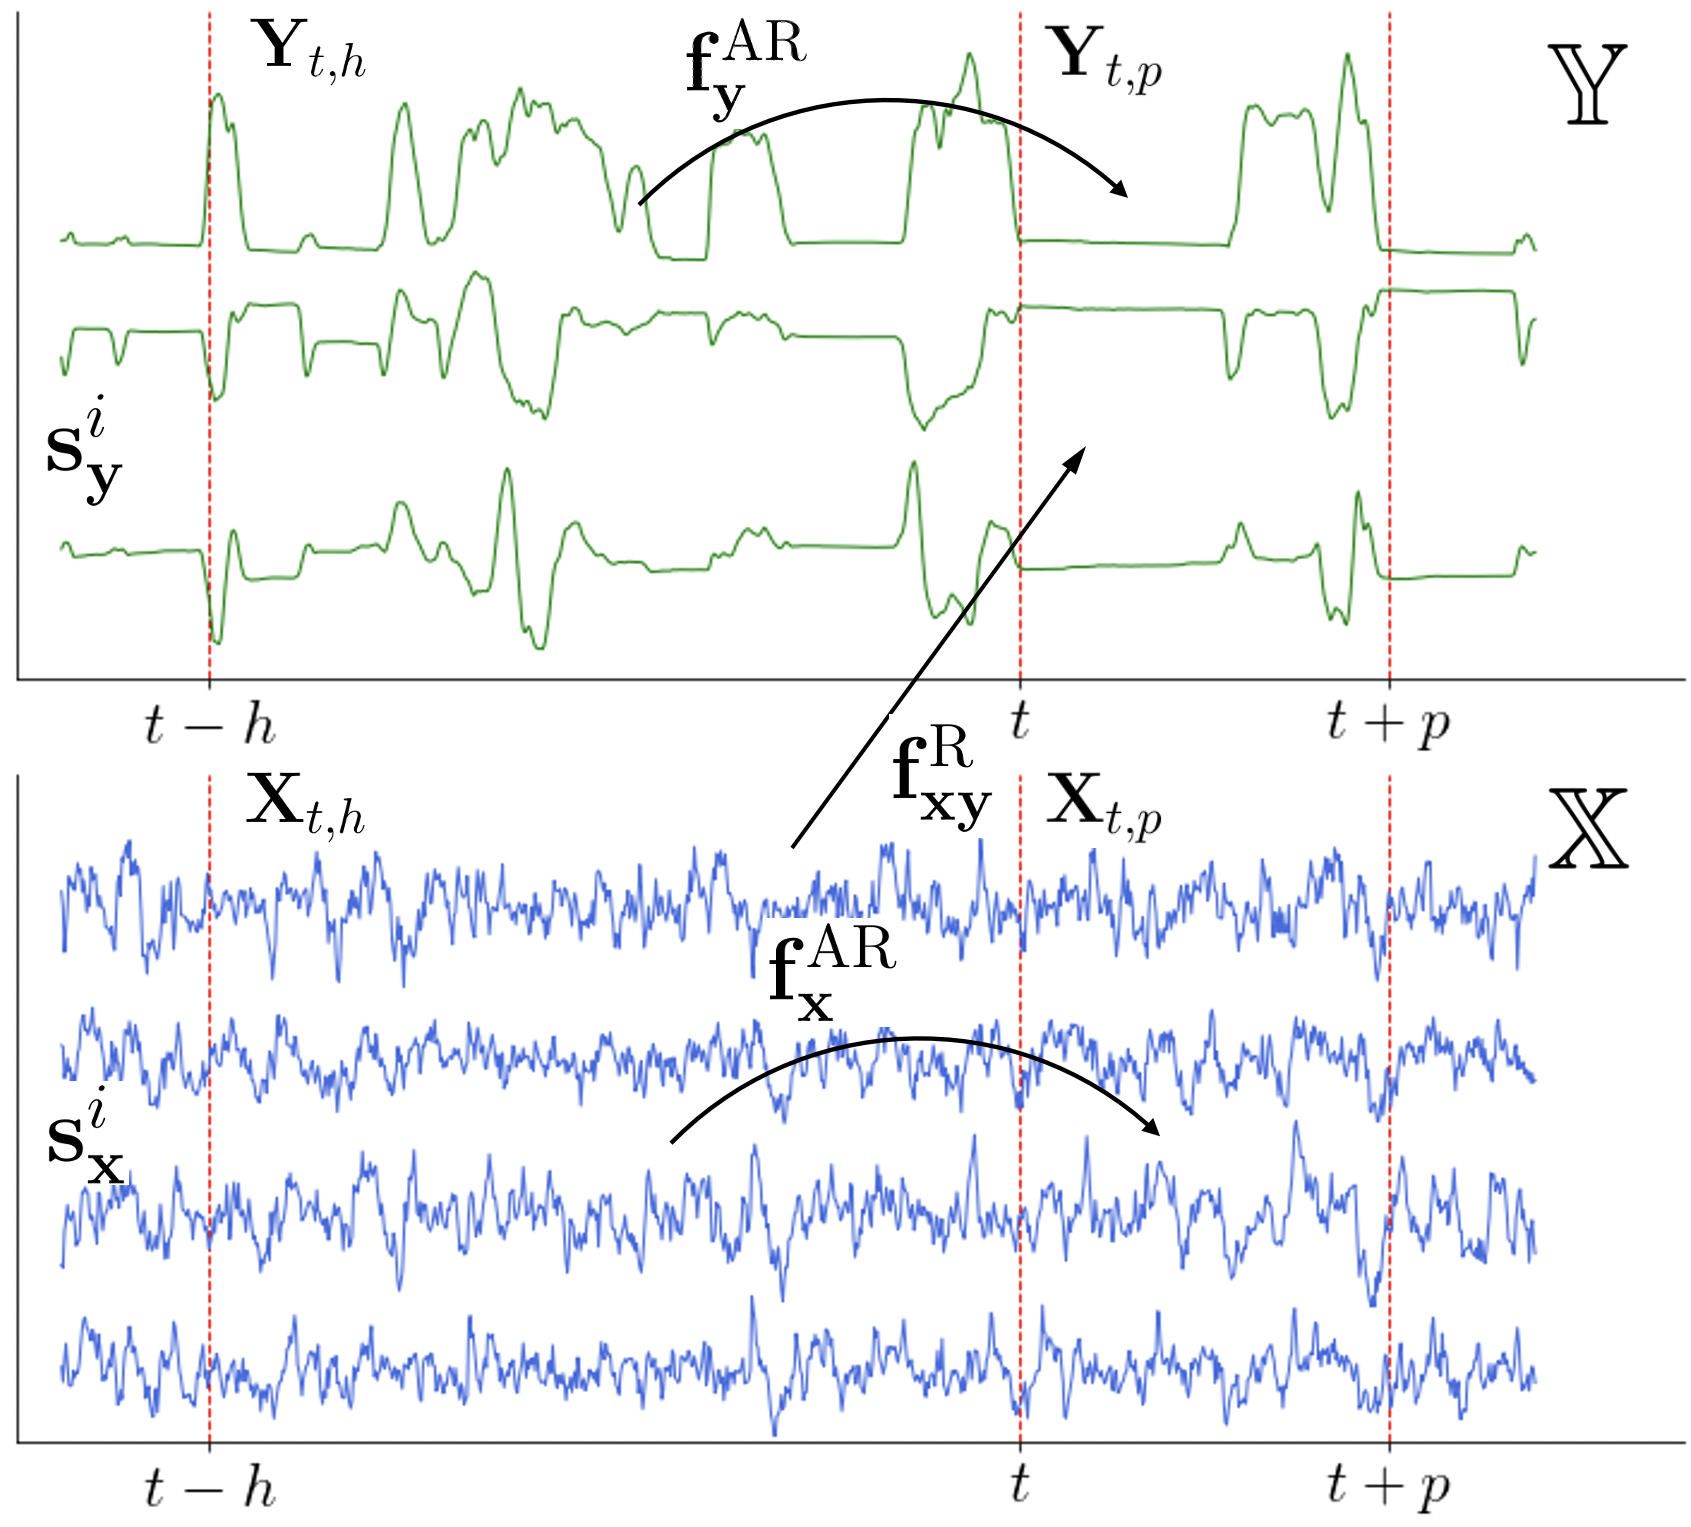
\includegraphics[width=0.7\linewidth]{figs/ch1/time_series_decoding}
	\caption{Схема построения моделей декодирования}
	\label{ch1:fig:time_series_decoding}
\end{figure}

Для построения авторегрессионной модели декодирования временных рядов широко используются два класса линейных методов: авторегрессионные модели и модели скользящего среднего~\cite{box2011time,hipel1994time}. 
Авторегрессионные модели AR($p$) строят прогноз в виде линейной комбинации $p$ предыдущих значений временного ряда.
Модели скользящего среднего MA($q$) вместо предыдущих значений временного ряда используют комбинацию ошибок.
Модель ARMA($p$, $q$)~\cite{cochrane2005time} является комбинацией двух описанных подходов. 
ARMA($p$, $q$) задает модель как линейную комбинацию $p$ предыдущих значений временного ряда и $q$ предыдущих значений ошибок. 
Для нахождения оптимальных параметров $p$ и $q$ модели ARMA используются автокорреляционная и частная автокорреляционная функции. 

Модель ARMA используется для стационарных временных рядов, отвечающим строгим статистическим предположениям. 
На практике встречается огромное количество нестационарных временных рядов подверженных тренду, сезонности или цикличности.
Модель ARIMA($p$, $d$, $q$)~\cite{cochrane2005time} обобщает модель ARMA для случая нестационарных временных рядов.
ARIMA берёт разности порядка $d$ от исходного временного ряда для достижения стационарности данных. 
При этом на практике оказывается достаточным положить $d = 1$.
Заметим, что при $d = 0$ модель ARIMA эквивалентна модели ARMA. 
Полезным обобщением модели ARIMA является модель AFRIMA~\cite{galbraith2001autoregression}. 
Модель позволяет задать параметр $d$ в виде вещественного числа.

Модель ARIMA плохо справляется с сезонными временными рядами.
В работе~\cite{box2011time} была предложена модель SARIMA, которая вводит в модель учет сезонной компоненты.

Задача декодирования временных рядов декомпозируется на следующие подзадачи.
\begin{itemize}
	\item Порождение признакового пространства. 
	Данный этап включает в себя процедуру извлечения признаков из исходных значений сигналов. 
	Процедура порождения признакового пространства может быть основана на экспертных знаниях или же являться моделью машинного обучения. 
	Данная подзадача подробно рассмотрена в главе~\ref{ch:metamodels}.
	
	\item Снижение размерности пространства или выбор признаков. 
	Исходные временные ряды, а также порожденное признаковое пространство оказывается избыточным, что приводит к избыточности и неустойчивости модели. 
	Методы снижения размерности и выбора признаков подробно изложены в главах~\ref{ch:pls} и~\ref{ch:qpfs}.
	
	\item Построение модели.
	После нахождения оптимального низкоразмерного представления исходных данных ставится задача выбора оптимальной модели декодирования.
\end{itemize}

%%%%%%%%%%%%%%%%%%%%%%%%%%%%%%%%%%%%%%%%%%%%%%%%
\textbf{Обзор методов снижения размерности для задачи декодирования.}
\label{sec:ch1:dim_reduction}
%%%%%%%%%%%%%%%%%%%%%%%%%%%%%%%%%%%%%%%%%%%%%%%%

Методы снижения размерности позволяют найти низкоразмерное представление исходных данных. 
Найденное представление используется для построения прогностической модели.
При этом метод снижения размерности может учитывать как зависимости в исходном объекте~$\bx$, так и в целевом объекте~$\by$.

\vspace{0.5cm}
\textbf{Метод главных компонент для задачи декодирования.}
Для устранения линейной зависимости и снижения размерности исходного пространства объектов широко используется метод главных компонент~(principal component analysis, PCA). 
Метод PCA находит низкоразмерное представление матрицы~$\bX = \bT \bP^{\T}$, такое что новое представление~$\bT \in \bbR^{m \times l}$ содержит максимальную долю дисперсии исходной матрицы.
При этом матрица отображения $\bP \in \bbR^{n \times l}$ является ортогональной ($\bP^{\T} \bP = \bI$) и содержит правые собственные вектора матрицы ковариаций $\bX^{\T} \bX$.

Метод PCA является базовым методом снижения размерности пространства. 
Существует множество модификаций базового метода.
Bероятностный PCA~\cite{tipping1999probabilisticpca} рассматривает задачу снижения размерности в терминах вероятностной модели, решая задачу с помощью вариационного EM алгоритма. 
Разреженный PCA~\cite{zou2006sparsepca} вводит в постановку задачи lasso регуляризацию для того, чтобы сделать матрицу отображения~$\bP$ разреженной и более интерпретируемой.
Нелинейный ядерный PCA~\cite{scholkopf1997kernelpca} отображает исходные данные с помощью нелинейного отображения и использует RKHS для решения исходной задачи.

После нахождения матрицы отображения $\bP$ задача~\eqref{ch1:eq:l2_loss_function} принимает вид

\begin{equation}
	\cL(\bB, \bT, \bY) = {\left\| \underset{m \times r}{\mathbf{Y}}  - \underset{m \times l}{\bT} \cdot \underset{l \times r}{\bB} \right\| }_2^2 \rightarrow\min_{\bB}.
	\label{ch1:eq:l2_loss_function_pca}
\end{equation}

Модель прогнозирования~\eqref{ch1:eq:lin_reg_model} в случае снижения размерности с помощью PCA принимает вид:
\begin{equation}
	\by = \bB \bt + \bepsilon = \bB \bP \bx + \bepsilon = \bTheta \bx + \bepsilon, \, \text{ где } \bTheta = \bB \bP.
	\label{ch1:eq:lin_reg_model_pca}
\end{equation}

\vspace{0.5cm}
\textbf{Метод частичных наименьших квадратов для задачи декодирования.}
Основным недостатком метода PCA является отсутствие учёта взаимосвязи между исходными признаками~$\bchi_j$ и целевыми векторами~$\bnu_j$.
Метод частичных наименьших квадратов (partial least squares, PLS) проецирует матрицу объектов~$\bX$ и матрицу ответов~$\bY$ в скрытое пространство малой размерностью~$l$ ($l < n$).
Метод PLS находит в скрытом пространстве матрицы~$\bT, \bU \in \bbR^{m \times l}$, которые лучше всего описывают исходные матрицы~$\bX$ и~$\bY$. 
При этом PLS максимизирует ковариацию между столбцами матриц $\bT$ и $\bU$ соответственно.

Метод PLS был впервые предложен в работах~\cite{wold1975path,wold1984collinearity,wold1982pls}. Подробное описание алгоритма приведено в работах~\cite{geladi1986partial,geladi1988notes,de1993simpls,vinzi2010handbook,brereton2014partial}.
В работах~\cite{rosipal2005overview,rosipal2011nonlinear} приведен обзор обобщений базовой модели PLS.
В работе~\cite{chun2010sparse} приведена модификация метода PLS для получения разреженного набора признаков. 
 

Матрица исходных объектов $\bX$ и матрица целевых объектов $\bY$ проецируются на скрытое пространство следующим образом:

\begin{align}
	\label{ch1:eq:PLS_X}
	\underset{m \times n}{\bX} 
	&= \underset{m \times l}{\bT} \cdot \underset{l \times n}{\bP^{\T}} + \underset{m \times n}{\bE_{\bx}} 
	= \sum_{k=1}^l \underset{m \times 1}{\btau_k} \cdot \underset{1 \times n}{\bp_k^{\T}} + \underset{m \times n}{\bE_{\bx}},\\
	\label{ch1:eq:PLS_Y}
	\underset{m \times r}{\bY} 
	&= \underset{m \times l}{\bU} \cdot \underset{l \times r}{\bQ^{\T}} + \underset{m \times r}{\bE_{\by}}
	=  \sum_{k=1}^l  \underset{m \times 1}{\bnu_k} \cdot \underset{1 \times r}{\bq_k^{\T}} +  \underset{m \times r}{\bE_{\by}}.
\end{align}

Здесь $\bT$ и $\bU$~--- образы исходных матриц в скрытом пространстве, причём столбцы матрицы $\bT$ ортогональны; $\bP$ и $\bQ$~--- матрицы перехода; $\bE_{\bx}$ и $\bE_{\by}$~--- матрицы остатков. 
Метод PLS максимизирует линейную зависимость между столбцами матриц~$\bT$ и~$\bU$
\begin{equation*}
	\bU \approx \bT \bB, \quad \bB = \text{diag}(\beta_k), \quad \beta_k = \bnu_k^{\T}\btau_k / (\btau_k^{\T}\btau_k),
\end{equation*}
где $\{\btau\}_{i=1}^l$, $\{\bnu\}_{i=1}^l$~--- столбцы матриц $\bT$ и $\bU$ соответственно.

Метод решает следующую оптимизационную задачу:
\begin{equation}
	\max_{\|\bp\|_{2}=\|\bq\|_{2}=1}[ \text{cov}(\bX \bp, \bY \bq)^{2}] = \max_{\bp, \bq} \frac{\bp^{\T} \bX^{\T} \bY \bq}{\sqrt{\bp^{\T} \bp} \sqrt{\bq^{\T} \bq}}.
	\label{ch1:eq:pls_max_cov}
\end{equation}

Детальное описание метода PLS с доказательством его корректности приведено в разделе~\ref{sec:ch2:pls_proof}.

Для демонстрации разницы между методами PCA, PLS был проведен модельный эксперимент для случая, когда размерности пространств исходных объектов, целевых объектов и скрытого пространства равны 2 ($n = r = l = 2$).
На Рис.~\ref{ch1:fig:pls_toy_example} показаны результаты работы методов. 
Синими и зелёными точками изображены исходные объекты~$\bx_i$ и целевые объекты~$\by_i$. 
Точки $\bX$ сгенерированы из нормального распределения с нулевым матожиданием. 
Точки $\bY$ линейным образом зависят от второй  главной компоненты $pc_2$ матрицы $\bX$ и не зависят от первой главной компоненты $pc_1$.
Красным контуром показаны линии уровня матриц ковариаций распределений. 
Черным изображены единичные окружности. 
Красные стрелки соответствуют главным компонентам матриц~$\bX$ и~$\bY$. 
Черные стрелки соответствуют векторам матриц~$\bW$ и~$\bC$ метода PLS. 
Данные матрицы содержат вектора, являющиеся аналогами главных компонент метода PCA.
Учёт взаимной связи между матрицами~$\bX$ и~$\bY$ отклоняет вектора~$\bw_k$ и~$\bc_k$ от направления главных компонент. 

При снижении размерности пространств до одного признака метод PCA выберет первую главную компоненту $pc_1$, отбросив компоненту $pc_2$, так как первая компонента объясняет большую часть дисперсии исходной матрицы $\bX$. 
При этом матрица $\bY$ не зависит от $pc_1$. 
Тем самым финальная модель окажется не адекватной.
Метод PLS позволяет побороться с данной проблемой.

\vspace{0.5cm}
\textbf{Канонический анализ корреляций для задачи декодирования.}
Канонический корреляционный анализ (canonical correlation analysis, CCA) широко применяется для поиска взаимосвязи между двумя наборами переменных~\cite{hotelling1992relations,anderson1962introduction}. 
Оптимизационная задача CCA похожа на оптимизационную задачу PLS~\eqref{ch1:eq:pls_max_cov} с той лишь разницей, что вместо максимизации ковариации CCA максимизирует корреляцию:
\begin{equation}
	\max_{\|\bp\|_{2}=\|\bq\|_{2}=1}[ \text{corr}(\bX \bp, \bY \bq)^{2}] = \max_{\bp, \bq} \frac{\bp^{\T} \bX^{\T} \bY \bq}{\sqrt{\bp^{\T} \bX^{\T}  \bX \bp} \sqrt{\bq^{\T} \bY^{\T}  \bY\bq}}.
	\label{ch1:eq:cca_max_corr}
\end{equation}

На Рис.~\ref{ch1:fig:cca_toy_example} показан результат работы метода. 
Основное различие состоит в том, что вектора $\bc_1$ и $\bc_2$ в данном случае становятся ортогональными.

В таблице~\ref{ch1:tbl:toy_example_results} приведены значения квадратичной ошибки $\mathcal{L}(\bTheta, \bX, \bY)$ для методов линейной регрессии, PCA, PLS и CCA.
Линейная регрессия отлично справляется с данной задачей.
Ошибка метода PCA наибольшая, что подтверждает факт, что для данной ситуации метод не находит нужных зависимостей в пространстве целевой переменной. 
Методы PLS и CCA показывают схожие результаты.

\begin{table}[]
	\centering
	\begin{tabular}{|c|c|c|c|}
		\hline
		\textbf{Линейная регрессия} & \textbf{PCA}   & \textbf{PLS}  &  \textbf{CCA}  \\ \hline
		0.01 &  0.24   &  0.13 &  0.13 \\ \hline
	\end{tabular}
	\caption{Средняя квадратичная ошибка на модельном примере для методов линейной регрессии, PCA, PLS, CCA}
	\label{ch1:tbl:toy_example_results}
\end{table} 

Нелинейный ядерный CCA~\cite{akaho2006kernel,melzer2001nonlinear,bach2002kernel,hardoon2004canonical} является обобщением базового метода. 
CCA и ядерный CCA широко используются для задач обучения без учителя~\cite{hardoon2007unsupervised,vinokourov2003inferring}. 
Метод имеет область применения от анализа хемометрических~\cite{montanarella1995chemometric} и биологических~\cite{vert2003graph} данных до обработки естественного языка~\cite{haghighi2008learning,dhillon2011multi}, аудиосигналов~\cite{choukri1986adaptation,rudzicz2010adaptive} и компьютерного зрения~\cite{kim2007tensor}.

В работе~\cite{andrew2013deep} впервые было предложено обобщение метода CCA, работающего с нейросетями. 
Предложенный метод DeepCCA максимизирует корреляцию между представлениями, полученными на выходе нейросети:
\begin{multline}
	\max_{\|\bp\|_{2}=\|\bq\|_{2}=1}\left[ \text{corr}(\mathbf{g}_{\bx}(\bX, \bW_{\bx}) \cdot \bp, \mathbf{g}_{\by}(\bY, \bW_{\by}) \cdot \bq)^{2}\right] = \\ = \max_{\bp, \bq} \frac{\bp^{\T} \mathbf{g}_{\bx}(\bX, \bW_{\bx})^{\T} \mathbf{g}_{\by}(\bY, \bW_{\by}) \bq}{\sqrt{\bp^{\T} \mathbf{g}_{\bx}(\bX, \bW_{\bx})^{\T}  \mathbf{g}_{\bx}(\bX, \bW_{\bx}) \bp} \sqrt{\bq^{\T} \mathbf{g}_{\by}(\bY, \bW_{\by})^{\T}  \mathbf{g}_{\by}(\bY, \bW_{\by}) \bq}}.
	\label{ch1:eq:depp_cca_max_corr}
\end{multline}
Здесь $\mathbf{g}_{\bx}(\bX, \bW_{\bx})$ и $\mathbf{g}_{\by}(\bY, \bW_{\by})$~--- нелинейные проекции исходных и целевых объектов.
В статье~\cite{wang2015deep} приведен обширный обзор модификаций нейросетевого CCA для работы с многовидовыми данными.
С использованием нейросетевых функций модель декодирования способна учитывать существенно нелинейные зависимости как в исходном пространстве, так и в целевом пространстве.
Главным недостатком нейросетевого CCA является вычислительная сложность. 
В работе~\cite{chang2018scalable} предложена релаксация исходной функции потерь, которая способна масштабироваться под работу с большими глубокими моделями нейросетей.

\vspace{0.5cm}
\textbf{Тензорные линейные методы для задачи декодирования.}
Если исходный объект $\bx$ является не вектором, а тензором более высокого порядка, то для построения модели тензор может быть вытянут в вектор~\cite{cichocki2009nonnegative}. 
В таком случае модель не учитывает имеющиеся зависимости между различными направлениями исходного тензора.
Для учета таких зависимостей используются тензорные версии метода PLS~\cite{zhao2012higher,eliseyev2013recursive,eliseyev2016penalized}.


\vspace{0.5cm}
\textbf{Многомодальные данные в задаче декодирования.}
Исходный объект может иметь несколько модальностей. 
Примерами таких модальностей могут быть выровненные аудио и видео~\cite{kidron2005pixels,chaudhuri2009multi}, аудио и артикуляция~\cite{arora2012kernel}, изображение и текстовая аннотация~\cite{hardoon2004canonical,socher2010connecting,hodosh2013framing}, параллельный корпус текстов~\cite{vinokourov2003inferring,haghighi2008learning,ap2014autoencoder,faruqui2014improving}.

В случае если для каждого объекта имеется более двух модальностей, то для построения скрытого пространства применяются два класса подходов. 
Первый подход состоит в построении скрытого пространства для каждой пары модальностей объекта~\cite{masci2013multimodal,rajendran2015bridge}. 
Второй же подход состоит в построении общего единого скрытого пространства для всех модальностей~\cite{kumar2011co,sharma2012generalized}.

\textbf{Глава 2. Задача построения согласованных моделей декодирования}

В данной главе приводится формальная постановка задачи декодирования в терминах проекций в скрытое пространство. 
Вводятся понятия скрытого пространства и процедуры согласования образов.
Доказываются теоремы о выборе оптимальной модели декодирования.

%%%%%%%%%%%%%%%%%%%%%%%%%%%%%%%%%%%%%%%%%%%%%%%%
\textbf{Процесс согласования моделей в пространстве высокой размерности.}
\label{sec:ch2:concordance}
%%%%%%%%%%%%%%%%%%%%%%%%%%%%%%%%%%%%%%%%%%%%%%%%

Для постановки задачи декодирования введём предположения о структурах пространств $\bbX$ и $\bbY$.
\begin{assumption}
	Рассмотрим случай, когда пространства $\bbX$ и $\bbY$ имеют избыточную размерность. 
	Это означает, что объекты $\bx$ и $\by$ принадлежат некоторым многообразиям низкой размерности. В простейшем случае такие многообразия могут являться вложениями или линейными подпространствами.
\end{assumption}

\begin{definition}
	Назовём пространство $\bbT \subset \bbR^l$ \textit{скрытым пространством} для пространства $\bbX \subset \bbR^n$ ($l \leq n$), если существуют функция $\bphi_{\bx}: \bbX \to \bbT$ и функция $\bpsi_{\bx}: \bbT  \to \bbX$ такие что
	\[
		\text{для любого } \bx \in \bbX \quad \text{существует } \bt \in \bbT: \bpsi_{\bx} (\bphi_{\bx}(\bx)) = \bpsi_{\bx}(\bt) = \bx.
	\]
	Функцию $\bphi_{\bx}(\bx)$ назовём \textit{функцией кодирования} объекта $\bx$, функцию $\bpsi_{\bx}(\bt)$  назовём \textit{функцией декодирования}. 
	
	Аналогично введём определение \textit{скрытого пространства}~$\bbU \subset \bbR^s$ для целевого пространства $\bbY$, \textit{функции кодирования} $\bphi_{\by}: \bbY \to \bbU$ и \textit{декодирования} $\bpsi_{\by}: \bbU  \to \bbY$ такие что
	\[
	 	\text{для любого } \by \in \bbY \quad \text{существует } \bu \in \bbU: \bpsi_{\by} (\bphi_{\by}(\by)) = \bpsi_{\by}(\bu) = \by.
	\]
\end{definition}

Образы матрицы исходных объектов~$\bX$ и матрицы целевых объектов~$\bY$ в скрытых пространствах~$\bbT$ и $\bbU$ имеют вид
\begin{align*}
	\bT &= \bphi_{\bx} (\bX) = [\bt_1, \dots, \bt_m]^{\T} = [\btau_1, \dots, \btau_l], \\
	\bU &= \bphi_{\by} (\bU) = [\bu_1, \dots, \bu_m]^{\T} = [\bnu_1, \dots, \bnu_s].
\end{align*}
Здесь строки $\{\bt_i\}_{i=1}^m$ матрицы~$\bT$ и строки $\{\bu_i\}_{i=1}^m$ матрицы~$\bU$ являются образами исходных объектов $\{\bx_i\}_{i=1}^m$ и целевых объектов $\{\by_i\}_{i=1}^m$. Столбцы $\{\btau_j\}_{j=1}^l$ матрицы~$\bT$ и столбцы $\{\bnu_j\}_{j=1}^s$ матрицы~$\bU$ являются скрытыми векторами.

\begin{definition}
	Будем говорить, что скрытые пространства $\bbT$ и $\bbU$ являются \textit{согласованными}, если существует \textit{функция связи} $\bh: \bbT \rightarrow \bbU$, такая что
	\[
		\text{для любого } \bu \in \bbU \quad \text{существует } \bt \in \bbT:  \bu = \bh(\bt).
	\]
\end{definition}

\begin{assumption}
	Предположим, что в задаче прогнозирования~\eqref{ch1:eq:loss_min} пространства $\bbT$ и $\bbU$ являются скрытыми для пространств $\bbX$ и $\bbY$ соответственно. 
	Предположим также, что для данных скрытых пространств $\bbT$ и $\bbU$ существует функция связи~$\bh: \bbT \rightarrow \bbU$. Тогда выполнено
	\[
		\text{для любого } \by \in \bbY \quad \text{существует } \bx \in \bbX: \by = \bpsi_{\by}(\bu) = \bpsi_{\by}(\bh(\bt)) = \bpsi_{\by}(\bh(\bphi_{\bx}(\bx))),
	\]
	и общая схема задачи поиска согласованной модели декодирования принимает вид следующей коммутативной диаграммы:
	\begin{equation}
		\begin{tikzpicture}
			\matrix (m) [matrix of math nodes,row sep=3em,column sep=4em,minimum width=2em]
			{
				\bbX \subset \bbR^n & \bbY \subset \bbR^r \\
				\bbT \subset \bbR^\ell & \bbU \subset \bbR^s \\};
			\path[-stealth]
			(m-1-1) edge [black] node [black, above] {$\mathbf{f}$} (m-1-2)
			(m-2-1) edge [black, bend right=10] node [black, right] {$\bpsi_{\bx}$} (m-1-1)
			(m-2-2) edge [black, bend left=10] node [black, left] {$\bpsi_{\by}$} (m-1-2)
			(m-1-1) edge [black, bend right=10] node [black, left] {$\bphi_{\bx}$} (m-2-1)
			(m-1-2) edge [black, bend left=10] node [black, right] {$\bphi_{\by}$} (m-2-2)
			(m-2-1) edge [black] node [black, above] {$\mathbf{h}$} (m-2-2);
		\end{tikzpicture}
		\label{ch2:eq:decoding_scheme}
	\end{equation}
\end{assumption}

\begin{definition}
	Согласно диаграмме~\eqref{ch2:eq:decoding_scheme}, определим \textit{согласованную} модель декодирования $\mathbf{f}: \bbX \rightarrow \bbY$ как суперпозицию
	\begin{equation}
		\mathbf{f} = \bpsi_{\by} \circ \bh \circ \bphi_{\bx}.
		\label{ch2:eq:def_decoding_function}
	\end{equation}
\end{definition}

Таким образом задача прогнозирования~\eqref{ch1:eq:loss_min} сводится к поиску согласованной модели декодирования~\eqref{ch2:eq:def_decoding_function}. 
Для поиска оптимальных параметров функций кодирования $\bphi_{\bx}$ и $\bphi_{\by}$, декодирования $\bpsi_{\bx}$ и $\bpsi_{\by}$, а также функции связи~$\bh$ ставится задача максимизации $\textit{функции согласования скрытых векторов}$
\[
	g: \bbR^m \times \bbR^m \rightarrow \bbR, \quad g(\btau, \bnu) \rightarrow \max_{\bphi_{\bx}, \bphi_{\by}, \bh}.
\]
Каждая пара скрытых векторов $\btau, \bnu$ ищется последовательно.

Сформулируем примеры методов снижения размерности пространства, описанные в разделе~\ref{sec:ch1:dim_reduction}, в терминах задачи построения согласованной модели декодирования.

\textbf{Метод главных компонент.} 
Метод главных компонент снижает размерность исходных данных и сохраняет максимальную дисперсию между полученными проекциями. 
Линейная модель PCA представляет собой ортогональное линейное преобразование исходного признакового пространства в скрытое пространство меньшей размерности. 

Функции кодирования $\bphi_{\bx}: \bbR^m \to \bbR^l$ и декодирования $\bpsi_{\bx}: \bbR^l \to \bbR^m$ имеют вид
\begin{equation*}
	\bphi_{\bx}(\bX) =  \underset{n \times m}\bX \cdot \underset{m \times l}\bP^{\T}, \quad	\bpsi_{\bx}(\bT) =  \underset{n \times l}\bT \cdot \underset{l \times m}\bP,
	\label{ch2:eq:PCA2}
\end{equation*}
где $\bP = [\bp_1, \dots, \bp_l].$ 
Здесь матрица $\bP$ является ортогональной матрицей, то есть $\bP^{-1} = \bP^{\T}$.

Скрытые вектора $\btau$ строятся так, чтобы выборочная дисперсия столбцов проекций матрицы~$\bX$ была максимальной:
\begin{equation*}
	\bp = \argmax_{\|\bp\|_{2} = 1} g(\btau) = \argmax_{\|\bp\|_{2} = 1} [\text{var}(\btau)] = \argmax_{\|\bp\|_{2} = 1} [\text{var}(\bX \textbf{p})],
\end{equation*}
где $\text{var}(\btau)$~--- выборочная дисперсия.

Метод PCA не согласует исходные переменные и целевые переменные. 
А именно метод PCA не находит функции кодирования $\bphi_{\by}$ и декодирования $\bpsi_{\by}$, а также функцию связи $\bh$. 
При этом функция согласования скрытых векторов $g(\btau)$ зависит только от одного аргумента.
Из-за этого зависимости в обоих пространствах не учитываются.
Пример некорректной работы  метода в случае наличия зависимостей как в исходном, так и в целевом пространстве, показан в разделе~\ref{sec:ch1:dim_reduction}.

\textbf{Метод наименьших частичных квадратов и канонический анализ корреляций.}
В методах PLS и CCA функции кодирования и декодирования имеют вид
\begin{align*}
	\bphi_{\bx}(\bX) &= \bX \bW, \quad \bphi_{\by}(\bY) = \bY \bC, \\
	\bpsi_{\bx}(\bT) &= \bT \bP^{\T}, \quad \bpsi_{\by}(\bU) = \bU \bQ^{\T}.
\end{align*}
Функция связи $\bh$ имеет вид линейной модели, связывающей образы проекций в скрытом пространстве $\bu = \bh(\bt) = \bB^{\T} \bt$.
В данном случае схема декодирования~\eqref{ch2:eq:decoding_scheme} принимает вид следующей коммутативной диаграммы.
\begin{equation*}
	\begin{tikzpicture}
		\matrix (m) [matrix of math nodes,row sep=3em,column sep=4em,minimum width=2em]
		{
			\bbX \subset \bbR^n & \bbY \subset \bbR^r \\
			\bbT \subset \bbR^\ell & \bbU \subset \bbR^s \\};
		\path[-stealth]
		(m-1-1) edge [black] node [black, above] {$\mathbf{f}$} (m-1-2)
		(m-1-1) edge [black, bend right=10] node [black, left] {$\bW$} (m-2-1)
		(m-2-1) edge [black, bend right=10] node [black, right] {$\bP$} (m-1-1)
		(m-1-2) edge [black, bend left=10] node [black, right] {$\bC$} (m-2-2)
		(m-2-2) edge [black, bend left=10] node [black, left] {$\bQ$} (m-1-2)
		(m-2-1) edge [black] node [black, above] {$\bB$} (m-2-2);
	\end{tikzpicture}
\end{equation*}
В разделе~\ref{sec:ch2:pls_proof} приводится подробная процедура нахождения оптимальных матриц $\bP$, $\bQ$, $\bW$, $\bC$, $\bB$ с доказательством корректности.

Различие между методами PLS и CCA заключается в виде функции согласования $g$.
Для метода PLS функция согласования скрытых векторов имеет вид $g(\btau, \bnu) = \text{cov}(\btau, \bnu)$, а для метода CCA: $g(\btau, \bnu) = \text{corr}(\btau, \bnu)$.

\textbf{Нелинейный канонический анализ корреляций.}
Помимо линейных моделей декодирования рассматриваются нелинейные методы. 
В данном случае функции кодирования и декодирования являются нелинейными нейросетями вида
\begin{align*}
	\bT &= \bphi_{\bx}(\bX) =  \bW_\bx^L \sigma(\dots \sigma(\bW_\bx^2 \sigma(\bX \bW_\bx^1)) \dots ), \\
	\bU &= \bphi_{\by}(\bY) =  \bW_\by^L \sigma(\dots \sigma(\bW_\by^2 \sigma(\bY \bW_\by^1)) \dots ), \\
	\bX &= \bpsi_{\bx}(\bT) =  \bW_\bt^L \sigma(\dots \sigma(\bW_\bt^2 \sigma(\bT \bW_\bt^1)) \dots ), \\
	\bY &= \bpsi_{\by}(\bU) =  \bW_\bu^L \sigma(\dots \sigma(\bW_\bu^2 \sigma(\bU \bW_\bu^1)) \dots ).
\end{align*}
Каждая нейросеть является суперпозицией последовательных умножений на матрицы параметров и применения поэлементных функций активаций.

Требуется найти такие параметры, при которых функция согласования~$g$ достигает своего максимума:
\begin{equation}
	g(\btau, \bnu) \rightarrow \max_{\bW},
	\label{ch2:eq:concordance}
\end{equation}
где $\bW = \bigl\{\bW_\bx^i, \bW_\by^i, \bW_\bt^i, \bW_\bu^i\bigr\}_{i=1}^L$.

Процесс согласования заключается в максимизации функции согласования $g(\btau, \bnu)$ по параметрам нейросетей.
В работе~\cite{andrew2013deep} рассматривается частный случай задачи~\eqref{ch2:eq:concordance}. 
При использовании в качестве функции согласования корреляции между проекциями $g(\btau, \bnu) = \textnormal{corr}(\btau, \bnu)$ частная производная функции согласования по первому аргументу принимает вид
\[
	\frac{\partial g(\btau, \bnu)}{\partial \btau} = \frac{1}{m - 1} \left(\bSigma_1^{-1/2} \bU \bV^{\T} \bSigma_2^{-1/2} \bU - \bSigma_1^{-1/2} \bU \bD \bV^{\T} \bSigma_1^{-1/2} \right),
\]
где $\bU, \bD, \bV = \textnormal{SVD}(\bSigma)$, \, $\bSigma = \bSigma_1^{-1/2} \bSigma_{12} \bSigma_2^{-1/2} $, \, $\bSigma_1 = \frac{1}{m - 1} \bT \bT^{\T}$, \, $\bSigma_2 = \frac{1}{m - 1} \bU \bU^{\T}$, \, $\bSigma_{12} = \frac{1}{m - 1} \bT \bU^{\T}$.
Аналогичное выражение имеет частная производная по второму аргументу.
Полученное выражение для градиента позволяет построить эффективный алгоритм для решения задачи с использованием градиентных методов оптимизации.

%%%%%%%%%%%%%%%%%%%%%%%%%%%%%%%%%%%%%%%%%%%%%%%%
\textbf{Доказательство корректности алгоритма проекции в скрытое пространство.}
\label{sec:ch2:pls_proof}
%%%%%%%%%%%%%%%%%%%%%%%%%%%%%%%%%%%%%%%%%%%%%%%%

Псевдокод метода регрессии PLS приведен в алгоритме~\ref{ch2:pls_pseudocode}.
Алгоритм итеративно на каждом из $l$ шагов вычисляет по одному столбцу $\btau_k$, $\bnu_k$, $\bp_k$, $\bq_k$ матриц $\bT$, $\bU$, $\bP$, $\bQ$ соответственно. 
После вычисления следующего набора векторов из матриц $\bX$, $\bY$ вычитаются очередные одноранговые аппроксимации. 
При этом предполагается, что исходные матрицы~$\bX$ и~$\bY$ нормированы (имеют нулевое среднее и единичное среднее отклонение).

\begin{algorithm}[h]
	\caption{Алгоритм PLS}
	\label{ch2:pls_pseudocode}
	\begin{algorithmic}[1]
		\REQUIRE $\bX, \bY, l$;
		\ENSURE $\bT, \bP, \bQ$;
		\STATE нормировать матрицы $\bX$ и $\bY$ по столбцам
		\STATE инициализировать $\bnu_0$ (первый столбец матрицы $\bY$)
		\STATE $\bX_1 = \bX; \bY_1 = \bY$
		\FOR{$k=1,\dots, l$}
		\REPEAT
		\vspace{0.1cm}
		\STATE $\bw_k := \bX_k^{\T} \bnu_{k-1} / (\bnu_{k-1}^{\T} \bnu_{k-1}); \quad \bw_k: = \frac{\bw_k}{\| \bw_k \|}$
		\vspace{0.1cm}
		\STATE $\btau_k := \bX_k \bw_k$
		\vspace{0.1cm}
		\STATE $\bc_k := \bY_k^{\T} \btau_k / (\btau_k^{\T} \btau_k); \quad \bc_k: = \frac{\bc_k}{\| \bc_k \|}$
		\vspace{0.1cm}
		\STATE $\bnu_k := \bY_k \bc_k$
		\UNTIL{$\btau_k$ не стабилизируется}
		\vspace{0.1cm}
		\STATE $\bp_k:= \bX_k^{\T}\btau_k/(\btau_k^{\T}\btau_k),\ 
		\bq_k := \bY_k^{\T}\btau_k/(\btau_k^{\T}\btau_k)$
		\vspace{0.2cm}
		\STATE $\bX_{k+1} :=  \bX_k - \btau_k \bp_k^{\T}$
		\vspace{0.2cm}
		\STATE $\bY_{k + 1} :=  \bY_k - \btau_k \bq_k^{\T}$ 
		\ENDFOR
	\end{algorithmic}
\end{algorithm}

Вектора $\btau_k$ и $\bnu_k$ из внутреннего цикла aлгоритма~\ref{ch2:pls_pseudocode}
содержат информацию о матрице исходных объектов $\bX$ и матрице целевых объектов $\bY$ соответственно. 
Блоки из шагов (6)--(7) и шагов (8)--(9)~--- аналоги метода PCA для матриц $\bX$ и $\bY$~\cite{geladi1988pls}. 
Последовательное выполнение блоков позволяет учесть взаимную связь между матрицами $\bX$ и $\bY$.

Теоретическое обоснование метода PLS следует из следующих утверждений.
\begin{statement}
	Максимизации ковариации между векторами $\btau_k$ и $\bnu_k$ сохраняет дисперсию столбцов матриц~$\bX$ и~$\bY$ и учитывает их линейную зависимость.
\end{statement}
\begin{proof}
	Утверждение следует из равенства
	\[
	\text{cov} (\btau_k, \bnu_k) = \text{corr} (\btau_k, \bnu_k) \cdot \sqrt{\text{var}(\btau_k)} \cdot \sqrt{\text{var}(\bnu_k)}.
	\]
	Максимизация дисперсий векторов $\btau_k$ и $\bnu_k$ отвечает за сохранение информации об исходных матрицах, корреляция между векторами отвечает взаимосвязи между $\bX$ и~$\bY$. 
\end{proof}

Во внутреннем цикле алгоритма~\ref{ch2:pls_pseudocode} вычисляются нормированные вектора весов $\bw_k$ и $\bc_k$. 
Из данных векторов строятся матрицы весов $\bW$ и $\bC$ соответственно.

\begin{statement}
	В результате выполнения внутреннего цикла вектора $\bw_k$ и $\bc_k$ будут собственными векторами матриц $\bX_k^{\T} \bY_k \bY_k^{\T} \bX_k$ и $\bY_k^{\T} \bX_k \bX_k^{\T} \bY_k$, соответствующими максимальным собственным значениям.
	
	\begin{equation*}
		\bw_k \varpropto \bX_k^{\T} \bnu_{k-1} \varpropto \bX_k^{\T} \bY_k \bc_{k-1} \varpropto \bX_k^{\T} \bY_k \bY_k^{\T} \btau_{k-1} \varpropto \bX_k^{\T} \bY_k \bY_k^{\T} \bX_k \bw_{k-1},
	\end{equation*}
	\begin{equation*}
		\bc_k \varpropto \bY_k^{\T} \btau_k \varpropto \bY_k^{\T} \bX_k \bw_k \varpropto \bY_k^{\T} \bX_k \bX_k^{\T} \bnu_{k-1} \varpropto \bY_k^{\T} \bX_k \bX_k^{\T} \bY_k \bc_{k-1},
	\end{equation*}
	где символ $\varpropto$ означает равенство с точностью до мультипликативной константы. 
	\label{ch2:stat:eig}
\end{statement}
\begin{proof}
	Утверждение следует из того факта, что правила обновления векторов $\bw_k$, $\bc_k$ совпадают с итерацией алгоритма поиска максимального собственного значения. 
	Данный алгоритм основан на следующем факте.
	Если матрица $\mathbf{A}$ диагонализуема, $\bx$~--- некоторый вектор, то
	
	\[
	\lim_{k \rightarrow \infty} \mathbf{A}^k \bx = \lambda_{\max}(\mathbf{A}) \cdot \mathbf{v}_{\max},
	\]
	где $ \lambda_{\max} (\mathbf{A})$~--- максимальное собственное значение матрицы $\mathbf{A}$, $\mathbf{v}_{\max}$~--- собственный вектор матрицы $\mathbf{A}$, соответствующий~$\lambda_{\max} (\mathbf{A})$.
	
\end{proof}

\begin{statement}
	Обновление векторов по шагам (6)--(9) aлгоритма~\ref{ch2:pls_pseudocode} соответствует максимизации ковариации между векторами~$\btau_k$ и~$\bnu_k$.
\end{statement}
\begin{proof}
	Максимальная ковариация между векторами~$\btau_k$ и~$\bnu_k$ равна максимальному собственному значению матрицы~$\bX_k^{\T} \bY_k \bY_k^{\T} \bX_k$:
	\begin{align*}
		\max_{\btau_k, \bnu_k}  \text{cov} (\btau_k, \bnu_k)^2 &= \max_{\substack{\|\bw_k\|=1 \\ \|\bc_k\| = 1}} \text{cov} \left( \bX_k \bw_k, \bY_k \bc_k \right)^2 = \max_{\substack{\|\bw_k\|=1 \\ \|\bc_k\| = 1}} \text{cov} \left(\bc_k^{\T}  \bY_k^{\T} \bX_k \bw_k \right)^2 = \\
		&= \max_{\|\bw_k\| = 1} \text{cov} \left\|\bY_k^{\T} \bX_k \bw_k \right\|^2 = \max_{\|\bw_k\| = 1} \bw_k^{\T} \bX_k^{\T} \bY_k \bY_k^{\T} \bX_k \bw_k = \\
		& = \lambda_{\max} \left( \bX_k^{\T} \bY_k \bY_k^{\T} \bX_k \right),
	\end{align*}
	где~$\lambda_{\max} (\mathbf{A})$~--- максимальное собственное значение матрицы $\mathbf{A}$.
	Применяя утверждение~\ref{ch2:stat:eig}, получаем требуемое.
\end{proof}

После завершения внутреннего цикла на шаге (11) вычисляются вектора $\bp_k$, $\bq_k$ проецированием столбцов матриц $\bX_k$ и $\bY_k$ на вектор $\btau_k$. 
Для перехода на следующий шаг необходимо вычесть из матриц $\bX_k$ и $\bY_k$ одноранговые аппроксимации $\btau_k \bp_k^{\T}$ и $\btau_k \bq_k^{\T}$
\begin{align*}
	\bX_{k + 1} &= \bX_{k} - \btau_k \bp_k^{\T} = \bX - \sum_k \btau_k \bp_k^{\T}, \\
	\bY_{k + 1} &= \bY_{k} - \btau_k \bq_k^{\T} = \bY - \sum_k \btau_k \bq_k^{\T}.
\end{align*}
При этом каждый следующий вектор~$\btau_k$ оказывается ортогонален всем векторам~$\btau_j$, $j=1, \dots, k$.

Для получения прогнозов модели и нахождения параметров модели 
домножим справа формулу~\eqref{ch1:eq:PLS_X} на матрицу $\bW$. Строки матрицы невязок $\bE$ ортогональны столбцам матрицы $\bW$, поэтому 
\[
\bX \bW = \bT \bP^{\T} \bW.
\] 

Линейное преобразование между объектами в исходном и латентном пространстве имеет вид
\begin{equation}
	\bT = \bX \bW^*,
	\label{ch2:eq:W*}
\end{equation}
где $\bW^* = \bW (\bP^{\T} \bW)^{-1}$. 

Матрица параметров модели~\ref{ch1:eq:lin_reg_model} находится из уравнений~\eqref{ch1:eq:PLS_Y},~\eqref{ch2:eq:W*}
\begin{equation}
	\bY = \bT \bQ^{\T} + \bE = \bX \bW^* \bQ^{\T} + \bE = \bX \bTheta + \bE.
	\label{ch2:eq:pls_model}
\end{equation}
Таким образом, параметры модели~\eqref{ch1:eq:lin_reg_model} равны
\begin{equation*}
	\bTheta = \bW (\bP^{\T} \bW)^{-1} \bQ^{\T}.
\end{equation*}

Финальная модель~\eqref{ch2:eq:pls_model} является линейной, низкоразмерной в скрытом пространстве. 
Это снижает избыточность данных и повышает стабильность модели.

%%%%%%%%%%%%%%%%%%%%%%%%%%%%%%%%%%%%%%%%%%%%%%%%
\textbf{Аддитивная суперпозиция моделей декодирования.}
\label{sec:ch2:superposition}
%%%%%%%%%%%%%%%%%%%%%%%%%%%%%%%%%%%%%%%%%%%%%%%%

Пусть $\mathbf{f}_1(\bx_1, \bTheta_1)$, $\mathbf{f}_2(\bx_2, \bTheta_2)$~--- линейные модели декодирования сигналов. 
Рассмотрим аддитивную суперпозицию моделей декодирования, то есть модель~\eqref{ch1:eq:reg_model} вида
\begin{equation}
	\by = \mathbf{f}(\bx, \bTheta) + \bepsilon = \bTheta_1 \bx_1 + \bTheta_2 \bx_2 + \bepsilon,
	\label{ch2:eq:two_modal_reg_model}
\end{equation}
где объект $\bx = [\bx_1, \bx_2] \in \bbR^n$ состоит из двух подвекторов $\bx_1 \in \bbR^k$, $\bx_2 \in \bbR^{n - k}$. Тем самым матрица параметров $\bTheta \in \bbR^{n \times r}$ состоит из двух подматриц $\bTheta_1 \in \bbR^{k \times r}$, $\bTheta_2 \in \bbR^{n - k \times r}$. 

\begin{statement}
	\label{ch2:stat:two_modal_params}
	Матрица параметров $\bTheta$ для модели~\eqref{ch2:eq:two_modal_reg_model}, доставляющая минимум функции ошибки~\eqref{ch1:eq:l2_loss_function}, имеет вид:
	\begin{align*}
		\bTheta_1 &= (\bX_1^{\T} \bM_{\bX_2} \bX_1)^{-1} \bX_1^{\T} \bM_{\bX_2} \bY, \\
		\bTheta_2 &= (\bX_2^{\T} \bM_{\bX_1} \bX_2)^{-1} \bX_2^{\T} \bM_{\bX_1} \bY,
	\end{align*}
	где $\bM_{\bX_1} = (\bI - \bP_{\bX_1})$, $\bM_{\bX_2} = (\bI - \bP_{\bX_2})$, $\bP_{\bX_1} = \bX_1 (\bX_1^{\T} \bX_1)^{-1} \bX_1^{\T}$, $\bP_{\bX_2} = \bX_2 (\bX_2^{\T} \bX_2)^{-1} \bX_2^{\T}$.
\end{statement}

\begin{proof}
	Домножим уравнение $\bY = \bX \bTheta$ слева на матрицу $\bX{\T}$
	\[
		\bX^{\T} \bX \bTheta = \bX^{\T} \bY \quad \Rightarrow \quad
		\begin{cases*}
			\bX_1^{\T} \bX_1 \bTheta_1 + \bX_1^{\T} \bX_2 \bTheta_2 = \bX_1^{\T} \bY, \\
			\bX_2^{\T} \bX_1 \bTheta_1 + \bX_2^{\T} \bX_2 \bTheta_2 = \bX_2^{\T} \bY.
		\end{cases*}
	\]
	Выразим из этой системы параметры каждой отдельной модели в суперпозиции:
	\[
		\begin{cases}
			\bTheta_1 = (\bX_1^{\T} \bX_1)^{-1} \bX_1^{\T} (\bY - \bX_2 \bTheta_2), \\
			\bTheta_2 = (\bX_2^{\T} \bX_2 )^{-1}  \bX_2^{\T} (\bY - \bX_1 \bTheta_1).
		\end{cases}
	\]
	Подставим полученные выражения для $\bTheta_1$ и $\bTheta_2$ в исходную систему:
	\[
				\begin{cases*}
					\bX_1^{\T} \bP_{\bX_1} (\bY - \bX_2 \bTheta_2) + \bX_1^{\T} \bX_2 \bTheta_2 = \bX_1^{\T} \bY, \\
					\bX_2^{\T} \bX_1 \bTheta_1 + \bX_2^{\T}\bP_{\bX_2} (\bY - \bX_1 \bTheta_1) = \bX_2^{\T} \bY.
				\end{cases*}
	\]
	Выразив матрицы параметров, получим требуемые выражения.
\end{proof}

Заметим, что матрицы $\bP_{\bX_1}$ и $\bP_{\bX_2}$ являются матрицами проекций на подпространства, образованные линейными оболочками столбцов матриц $\bX_1$ и $\bX_2$ соответственно.
Таким образом матрицы $\bM_{\bX_1}$ и $\bM_{\bX_2}$ являются матрицами проекций на ортогональные подпространства.

\begin{statement}
	\label{ch2:stat:two_modal_theta2}
	Оптимальная подматрица $\bTheta_2$ в модели~\eqref{ch2:eq:two_modal_reg_model} является решением задачи регрессии
	\begin{equation}
		\| \bY_1 -  \bX_{21} \bTheta_2 \| \rightarrow \min_{\bTheta_2},
		\label{ch2:eq:two_modal_fwl}
	\end{equation}
	где $\bY_1 = \bM_{\bX_1} \bY$, $\bX_{21} = \bM_{\bX_1} \bX_2$.
\end{statement}

\begin{proof}
	Матрица $\bM_{\bX_1}$ является матрицей проекции на ортогональное подпространство, построенное на линейной оболочке столбцов матрицы $\bX_1$. Таким образом, матрица $\bM_{\bX_1}$ является идемпотентной ($\bM_{\bX_1}{\T} \bM_{\bX_1} = \bM_{\bX_1}$). 
	Таким образом, используя утверждение~\ref{ch2:stat:two_modal_params},
	\begin{multline*}
		\bTheta_2 = (\bX_2^{\T} \bM_{\bX_1} \bX_2)^{-1} \bX_2^{\T} \bM_{\bX_1} \bY = (\bX_2^{\T} \bM_{\bX_1}^{\T} \bM_{\bX_1} \bX_2)^{-1} \bX_2^{\T} \bM_{\bX_1}^{\T} \bM_{\bX_1} \bY = \\
		= ((\bM_{\bX_1} \bX_2)^{\T} (\bM_{\bX_1} \bX_2)^{\T})^{-1} (\bM_{\bX_1} \bX_2)^{\T} (\bM_{\bX_1} \bY) = (\bX_{21}^{\T} \bX_{21})^{-1} \bX_{21}^{\T} \bY_1.
	\end{multline*}
	Согласно теореме Гаусса-Маркова $\bTheta_2$ является решением задачи регрессии~\eqref{ch2:eq:two_modal_fwl}.
\end{proof}

Таким образом для нахождении оптимальной модели декодирования $\mathbf{f}(\bx_2, \bTheta_2)$ необходимо спроецировать матрицы $\bY$ и $\bX_2$ на подпространства, ортогональные подпространству, образованному линейной оболочкой столбцов матрицы $\bX_1$.

Похожие результаты были доказаны в эконометрике в работах~\cite{frisch1933partial,lovell1963seasonal,cinelli2020making}. Аналогичное утверждение верно и для матрицы~$\bTheta_1$. 

\begin{statement}
	Если в задаче~\eqref{ch2:eq:two_modal_reg_model} $\text{span}(\bX_1) \cap \text{ span}(\bX_2) = \emptyset$, то есть столбцы матрицы $\bX_1$ ортогональны столбцам матрицы~$\bX_2$, то $\bTheta_2$ является решением задачи регрессии
	\[
		\| \bY -  \bX_{2} \bTheta_2 \| \rightarrow \min_{\bTheta_2}.
	\]
\end{statement}

\begin{proof}
	Используя факт, что $\bI = \bP_{\bX_1} + \bM_{\bX_1}$ и $\bX_2 \bX_1 = 0$, получаем
	\begin{multline*}
		(\bX_2^{\T} \bX_2)^{-1} \bX_2^{\T} \bY = (\bX_2^{\T} \bX_2)^{-1} \bX_2^{\T} (\bP_{\bX_1} + \bM_{\bX_1}) \bY = \\ = (\bX_2^{\T} \bX_2)^{-1} \bX_2^{\T} \bM_{\bX_1} \bY  = (\bX_{21}^{\T} \bX_{21})^{-1} \bX_{21}^{\T} \bY_1.
	\end{multline*}
	Используя утверждение~\ref{ch2:stat:two_modal_theta2}, получаем требуемое утверждение.
\end{proof}
Данное утверждение показывает, что в случае независимых столбцов матриц $\bX_1$ и $\bX_2$ задача регрессии для аддитивной суперпозиции моделей~\eqref{ch2:eq:two_modal_reg_model} распадается на две независимые подзадачи.

Из выше доказанных утверждений прямо следует следующая теорема.

\begin{theorem}
	Если в задаче~\eqref{ch2:eq:two_modal_reg_model} $\text{span}(\bX_1) \neq \text{ span}(\bX_2)$, то ошибка аддитивной суперпозиции моделей не превышает ошибки каждой из отдельных моделей
	\begin{align*}
		\mathcal{L}(\bTheta^*, \bX, \bY) &\leq \mathcal{L}(\bTheta_1, \bX_1, \bY), \\
		\mathcal{L}(\bTheta^*, \bX, \bY) &\leq \mathcal{L}(\bTheta_2, \bX_2, \bY).
	\end{align*}
\end{theorem}

Рассмотрим случай линейной авторегрессионной модели $\mathbf{f}^{\text{AR}}_{\by}$ из определения~\ref{ch1:def:autoreg_model} и линейной регрессионной модели $\mathbf{f}^{\text{R}}_{\bx\by}$ из определения~\ref{ch1:def:reg_model}. 
Пусть модель декодирования $\mathbf{f}_{\bx\by}: \bbR^{h_x \times m} \times \bbR^{h_y \times r} \rightarrow \bbR^{p \times r}$ из определения~\ref{ch1:def:decode_model} является аддитивной суперпозицией авторегрессионной и регрессионной моделей.
Тогда при условии не совпадений подпространств, образованных линейными оболочками входами моделей, ошибка суперпозиции не будет превышать ошибок авторегрессионной и регрессионной моделей.
Данное утверждение позволяет осуществлять выбор моделей в суперпозиции, основанный на анализе проекций подпространств, построенных на линейных оболочках исходных признаковых описаний.

%%%%%%%%%%%%%%%%%%%%%%%%%%%%%%%%%%%%%%%%%%%%%%%%
\textbf{Анализ линейных методов проекции в скрытое пространство.}
\label{sec:ch2:exp_linear}
%%%%%%%%%%%%%%%%%%%%%%%%%%%%%%%%%%%%%%%%%%%%%%%%

Для проведения вычислительного эксперимента рассматриваются данные потребления электроэнергии.
Временные ряды электроэнергии состоят из почасовых записей (52512 наблюдений). 
Строка матрицы~$\bX$~--- локальная история сигнала за одну неделю $n = 24 \times 7$. 
Строка матрицы~$\bY$~--- локальный прогноз потребления электроэнергии в следующие 24 часа $r = 24$. 
В этом случае матрицы~$\bX$ и~$\bY$ являются авторегрессионными матрицами.

Вычислительный эксперимент также проводился на данных электрокортикограмм (ECoG) из проекта NeuroTycho~\cite{shimoda2012decoding}.
Данные ECoG состоят из 32-канальных сигналов напряжения, снятых с головного мозга.
Цель состоит в предсказании по входному сигналу ECoG 3D позиции рук в последующие моменты времени.
Исходные сигналы напряжения преобразуются в пространственно-временное представление с помощью вейвлет-преобразования с материнским вейвлетом Морле.
Процедура извлечения признаков из исходных данных подробно описана в~\cite{chao2010long,eliseyev2016penalized}.
Описание исходного сигнала в каждый момент времени имеет размерность 32 (каналы) $\times $ 27 (частоты) = 864.
Каждый объект представляет собой локальный отрезок времени длительностью $\Delta t = 1s$. 
Временной шаг между объектами $\delta t = 0.05 s$.
Матрицы имеют размеры $\bX \in \bbR^{18900 \times 864}$ и $\bY \in \bbR^{18900 \times 3k}$, где $k$~--- число отсчётов времени прогнозирования.
Данные разбиты на тренировочную и тестовую части в соотношении 0,67. 
Пример исходных сигналов мозга и соответствующей траектории руки показан на Рис.~\ref{ch2:fig:ecog_data}.

\begin{figure}[ht]
	\centering
	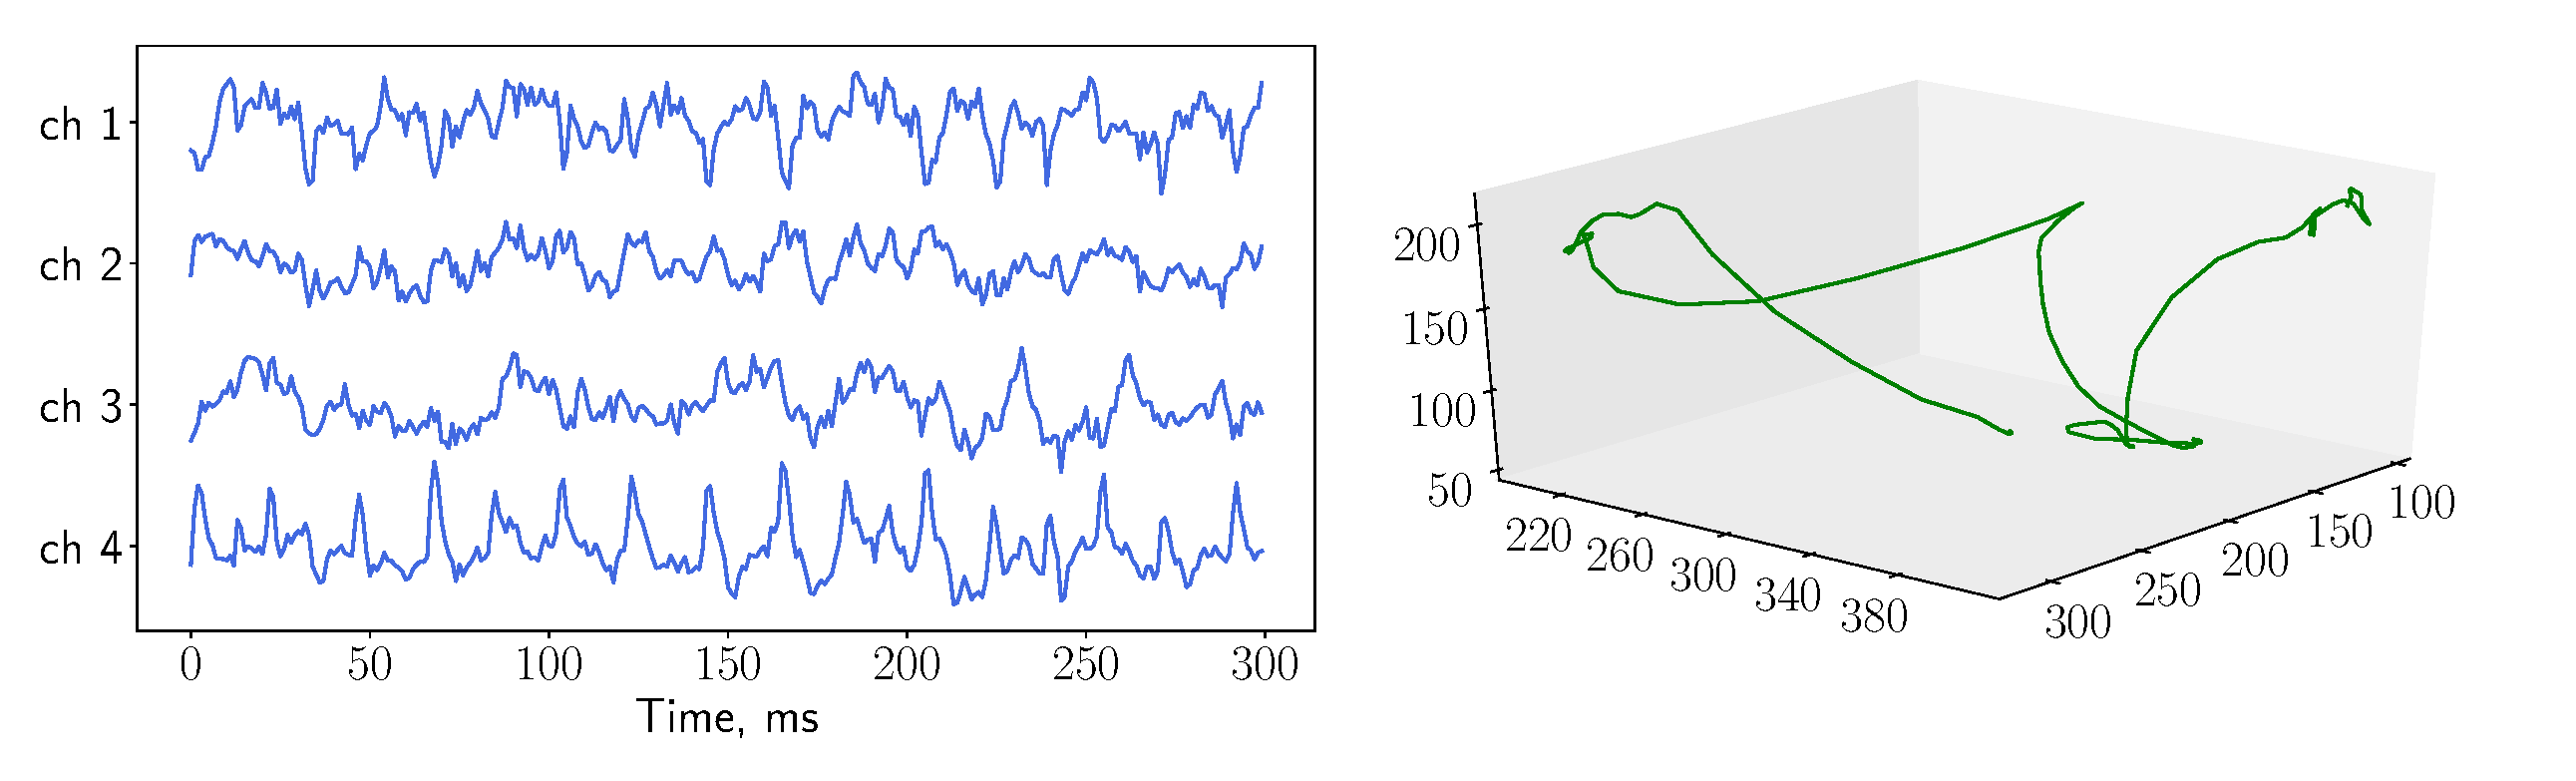
\includegraphics[width=\linewidth]{figs/ch2/ecog_data}
	\caption{Сигналы мозга (левый график) и 3D координаты руки (правый график)}
	\label{ch2:fig:ecog_data}
\end{figure}

Введём среднеквадратичную ошибку для некоторых матриц $\mathbf{A} = [a_{ij}]$ и $\mathbf{B} = [b_{ij}]$
\[
	\text{MSE} (\mathbf{A}, \mathbf{B}) = \sum_{i,j} (a_{ij} - b_{ij})^2.
\]
Для оценивания качества аппроксимации вычисляется значение нормированной среднеквадратичной ошибки
\begin{equation}
	\text{NMSE}(\bY,  \mathbf{\hat{Y}}) = \frac{\text{MSE} (\bY, \mathbf{\hat{Y}})}{\text{MSE} (\bY, \mathbf{\bar{Y}})},
	\label{ch2:eq:nmse}
\end{equation}
где $\mathbf{\hat{Y}}$~--- прогноз модели, $\mathbf{\bar{Y}}$~--- константный прогноз средним значением по столбцам матрицы.

\textbf{Результаты на данных электроэнергии.}
Для нахождения оптимальной размерности $l$ латентного пространства все данные потребления электроэнергии были разбиты на обучающую и валидационную части. 
Обучающая выборка состоит из $700$ объектов, валидационная из $370$. Зависимость нормированной квадратичной ошибки~\eqref{ch2:eq:nmse} от размерности $l$ латентного пространства представлена на Рис.~\ref{ch2:fig:energy_n_comp}. 
Сначала ошибка резко падает при увеличении размерности скрытого пространства, а затем стабилизируется.

Минимальная ошибка наблюдается при $l=14$. 
Построим прогноз потребления электроэнергии при данном $l$. 
Результат аппроксимации изображен на Рис.~\ref{ch2:fig:energy_prediction}. Алгоритм PLS восстановил авторегрессионную зависимость и обнаружил дневную сезонность.

\textbf{Результаты на данных электрокортикограммы.}
На Рис.~\ref{ch2:fig:ecog_n_comp} представлена зависимость нормированной квадратичной ошибки~\eqref{ch2:eq:nmse} от размерности латентного пространства. Ошибка аппроксимации меняется незначительно при $l > 5$.
Таким образом совместное описание пространственно-временного спектрального представления объектов и пространственного положения руки может быть представлено вектором размерности $l \ll n$.
Зафиксируем $l = 5$. 
Пример аппроксимации положения руки изображен на Рис.~\ref{ch2:fig:ecog_prediction}. 
Сплошными линиями изображены истинные координаты руки по всем осям, пунктирными линиями показана аппроксимация методом PLS.

%%%%%%%%%%%%%%%%%%%%%%%%%%%%%%%%%%%%%%%%%%%%%%%%
\section{Анализ нелинейных методов проекции в скрытое пространство}
\label{sec:ch2:exp_nonlinear}
%%%%%%%%%%%%%%%%%%%%%%%%%%%%%%%%%%%%%%%%%%%%%%%%

Цель вычислительного эксперимента~--- сравнительный анализ рассматриваемых моделей.
Рассматриваются данные, для которых сложность класса линейных методов неадекватно низка.
Нелинейные модели позволяют получить точный прогноз при адекватной сложности.

\textbf{Задача фильтрации шума.}
Проведем сравнение качества DeepCCA и CCA на задаче классификации зашумленных цифровых изображениях, представленных на Рис.~\ref{ch2:fig:noisy_mnist}. Для этого используется набор данных MNIST~\cite{MNIST}, который состоит из 70\,000 цифровых изображений $28 \times 28$ образцов рукописного написания цифр. Предлагается получить два новых набора данных $\bX$ и $\bY$ следующим образом. Первый набор получается поворотом исходных изображений на угол в диапазоне $[\frac{-\pi}{4}, \frac{\pi}{4}]$. Для получения второго набора данных для каждой картинки из первого набора данных ставится в соответствие случайным образом картинка с той же цифрой, но с добавлением независимого случайного шума, распределенного равномерно на отрезке $[0,1]$.

\begin{table}[ht]
	\caption{Точность классификации линейного SVM для методов Deep CCA и CCA}
	\centering
	\begin{tabular}{l|cc}
	\hline
		Скользящий контроль & Deep CCA ($L=3$) & CCA \\  \hline
		Валидация & 92,74\%  &  76,21\%\\
		Тест & 92,14\% & 76,07\% \\
		\hline
	\end{tabular}
	\label{ch2:tbl:svm_cca}
\end{table}

Применив к двум новым наборам данных DeepCCA или CCA, получаем новое низкоразмерное признаковое пространство, которое игнорирует шумы в исходных данных. Модель DeepCCA представляет собой нейронную сеть с $L=3$ скрытыми слоями. Таким образом, получаем функции кодирования $\bphi_{\bx}$ и $\bphi_{\by}$ для исходных наборов данных. На новых признаках, полученных разными моделями (DeepCCA и CCA), для первого набора данных, то есть на данных после применения функции кодирования $\bphi_{\bx}$ к первому набору исходных данных, обучим линейный SVM-классификатор. Показателем эффективности будет точность классификации линейного SVM на тестовых данных. В случае построения адекватного скрытого пространства полученные образы объектов будут линейно разделимы. Результаты эксперимента приведены в таблице~\ref{ch2:tbl:svm_cca}. Точность классификации нелинейной модели существенно выше линейного метода CCA.

\textbf{Задача восстановления изображений.}
Для анализа процедуры согласования проведен вычислительный эксперимент с предложенными нелинейными моделями.
Для снижения размерности пространства используются нейросетевые модели автоэнкодера c согласованием скрытого пространства~\eqref{ch2:eq:concordance}.
В качестве базовых моделей используются модель автоэнкодера без согласования скрытых пространств, а также линейный PLS. В качестве исходного набора данных используется набор данных MNIST~\cite{MNIST}. Каждое изображение поделено на левую и правую части, как показано на Рис.~\ref{ch2:fig:left_right_mnist}. Модель по левому изображению восстанавливает правое изображение.

Модель EncNet1~--- нейронная сеть с нелинейными функциями активации, которая обучается на данных после преобразования их автоэнкодером. Модель LinNet1~--- нейронная сеть с одним линейным слоем, которая также обучается на преобразованных данных. Для EncNet1 и LinNet1 автоэнкодеры для исходных и целевых объектов используют совместную функцию потерь, которая связывает выходы энкодеров. Модели EncNet2 и LinNet2 устроены аналогично EncNet1 и LinNet1 соответственно, но в автоэнкодерах нет совместной функции потерь. Модель DumbNet~---  нейронная сеть, которая обучается на исходных данных и имеет такую же структуру, что и EncNet, то есть имеет такое же число слоев и в каждом слое такое же количество нейронов, что и у EncNet.

Для оценки качества моделей вычислялась среднеквадратичная ошибка. Примеры восстановленных изображений показаны на Рис.~\ref{ch2:fig:mnist_nn_preds}. Качество моделей, а также их сложность представлены в таблице~\ref{ch2:tbl:mnist_nn_error}.
На Рис.~\ref{ch2:fig:mnist_nn_preds} показано, что предложенные модели EncNet и LinNet позволяют получить более четкие и различимые изображения, в отличие от базовой нелинейной модели DumbNet и линейной модели PLS.
Несмотря на заметное улучшение визуального качества изображений, ошибка предложенных моделей выше, чем у модели DumbNet.
Это связано с тем, что среднеквадратичная ошибка оказалась неадекватной метрикой в пространстве изображений.
Нахождение оптимальной метрики для оценки качества предложенных методов может быть одним из возможных направлений развития текущего эксперимента.

\begin{table}[!ht]
	\caption{Квадратичная ошибка для нелинейных моделей в задаче восстановления правой части изображения по левой}
	\centering
	\small
	\begin{tabular}{l|cccccc}
	\hline
		& EncNet1 & LinNet1 & EncNet2 & LinNet2 & DumbNet & PLS\\  \hline
		Число параметров, тыс. & 283 & 239 & 283 & 239  & 283 & --\\
		Ошибка на тесте & 0,147 & 0,235 & 0,149 & 0,236 & 0,128 & 0,188 \\
		\hline
	\end{tabular}
	\label{ch2:tbl:mnist_nn_error}
\end{table}

\textbf{Глава 3. Выбор признаков в задаче декодирования сигналов.}
\label{ch:qpfs}

Задача выбора признаков заключается в поиске оптимального подмножества~$\cA \subset \{ 1, \dots, n \}$ индексов признаков среди всех возможных $2^n - 1$ вариантов. 
Существует взаимооднозначное отображение между подмножеством $\cA$ и булевым вектором~$\ba \in \{0, 1\}^n$, компоненты которого указывают, выбран ли признак. 
Для нахождения оптимального вектора~$\ba$ введем функцию ошибки выбора признаков~$S(\ba, \bX, \bY)$. 
Проблема выбора признаков принимает вид:
\begin{equation}
	\ba = \argmin_{\ba' \in \{0, 1\}^n} S(\ba', \bX, \bY).
	\label{ch3:eq:feature_selection}
\end{equation}
Целью выбора признаков является построение функции~$S (\ba, \bX, \bY)$. Конкретные примеры данной функции для рассматриваемых методов выбора признаков приведены ниже и обобщены в таблице~\ref{ch3:tbl:summary}.

Задача~\eqref{ch3:eq:feature_selection} имеет дискретную область определения~$\{0, 1\}^n$. Для решения данной задачи применяется релаксация задачи~\eqref{ch3:eq:feature_selection} к непрерывной области определения~$[0, 1]^n$. Релаксированная задача выбора признаков имеет следующий вид:
\begin{equation}
	\bz = \argmin_{\bz' \in [0, 1]^n} S(\bz', \bX, \bY).
	\label{ch3:eq:relaxed_feature_selection}
\end{equation}

Здесь компоненты вектора~$\bz$~--- значения нормированных коэффициентов значимости признаков.
Сначала решается задача~\eqref{ch3:eq:relaxed_feature_selection}, для получения вектора значимостей~$\bz$. 
Затем решение~\eqref{ch3:eq:feature_selection} восстанавливается с помощью отсечения по порогу следующим образом:
\begin{equation}
	\ba = [a_j]_{j=1}^n, \quad 
	a_j = \begin{cases}
		1, & z_j > \tau; \\
		0, & \text{в противном случае}.
	\end{cases}
	\label{ch3:eq:feature_threshold}
\end{equation}
$\tau$~--- гиперпараметр, который может быть подобран вручную или выбран с помощью кросс-валидации. 

Как только решение~$\ba$ задачи~\eqref{ch3:eq:feature_selection} получено, задача~\eqref{ch1:eq:l2_loss_function} принимает вид:
\begin{equation*}
	\mathcal{L}(\bTheta_{\cA}, \bX_{\cA}, \bY) = {\left\| \mathbf{Y} - \bX_{\cA}\bTheta_{\cA} \right\| }_2^2 \rightarrow\min_{\bTheta_{\cA}},
\end{equation*}
где индекс~$\cA$ обозначает подматрицу со столбцами, индексы которых содержатся в~$\cA$.

%%%%%%%%%%%%%%%%%%%%%%%%%%%%%%%%%%%%%%%%%%%%%%%%
\textbf{Выбор признаков с помощью квадратичного программирования.}
\label{sec:ch3:qpfs_feature_selection}
%%%%%%%%%%%%%%%%%%%%%%%%%%%%%%%%%%%%%%%%%%%%%%%%

Если между столбцами матрицы исходных объектов~$\bX$ существует линейная зависимость, то решение задачи линейной регрессии
\begin{equation}
	\| \bupsilon - \bX \btheta\|_2^2 \rightarrow\min_{\btheta \in \bbR^{n}}.
	\label{ch3:eq:linear_regression}
\end{equation}
оказывается неустойчивым. 
Методы выбора признаков находят подмножество~$ \cA \in \{1, \dots, n\}$ оптимальных столбцов матрицы~$\bX$. 

Метод QPFS~\cite{rodriguez2010quadratic} выбирает некоррелированные признаки, релевантные целевому вектору~$\bupsilon$.
Чтобы формализовать этот подход, введем две функции: $\text{Sim}(\bX)$ и $\text{Rel}(\bX, \bupsilon)$. 
$\text{Sim}(\bX)$ контролирует избыточность между признаками, $\text{Rel}(\bX, \bupsilon)$ содержит релевантности между каждым признаком и целевым вектором. 
Мы хотим минимизировать функцию Sim и максимизировать Rel одновременно.

QPFS предлагает явный способ построения функций Sim и Rel. 
Метод минимизирует следующую функцию ошибки
\begin{equation}
	\underbrace{\bz^{\T} \bQ \bz}_{\text{Sim}} - \alpha \cdot \underbrace{\vphantom{()} \mathbf{b}^{\T} \bz}_{\text{Rel}} \rightarrow \min_{\substack{\bz \in \bbR^n_+ \\ \|\bz\|_1=1}}.
	\label{ch3:eq:qpfs_problem}
\end{equation}
Элементы матрицы парных взаимодействий~$\bQ \in \bbR^{n \times n}$ содержат коэффициенты попарного сходства между признаками. 
Вектор релевантностей признаков~$\mathbf{b} \in \bbR^n$ выражает сходство между каждым признаком и целевым вектором~$\bupsilon$.
Нормированный вектор~$\bz$ отражает значимость каждого признака. 
Функция ошибки~\eqref{ch3:eq:qpfs_problem} штрафует зависимые признаки функцией Sim и штрафует признаки, не релевантные к целевой переменной функцией Rel. 
Параметр~$\alpha$ позволяет контролировать компромисс между Sim и Rel.
Авторы оригинальной статьи QPFS~\cite{rodriguez2010quadratic} предложили способ выбора~$\alpha$, чтобы уравновесить вклад членов $\text{Sim}(\bX)$ и $\text{Rel}(\bX, \bupsilon)$

\begin{equation*}
	\alpha = \frac{\overline{\bQ}}{\overline{\bQ} + \overline{\bb}}, \quad \text{где}\,\,\overline{\bQ} = \text{mean} (\bQ), \,\,\, \overline{\bb}= \text{mean} (\bb).
\end{equation*}
Чтобы выделить оптимальное подмножество признаков, применяется отсечение по порогу~\eqref{ch3:eq:feature_threshold}.

Для измерения сходства используется выборочный коэффициент корреляции Пирсона между парами признаков для функции Sim, и между признаками и целевым вектором для функции Rel:
\begin{equation}
	\bQ = \left[|\text{corr}(\bchi_i, \bchi_j)|\right]_{i,j=1}^n, \quad \bb = \left[|\text{corr}(\bchi_i, \bupsilon)|\right]_{i=1}^n.
	\label{ch3:eq:qpfs_1d_qb}
\end{equation}
Здесь
\begin{equation*}
\text{corr}(\bchi, \bupsilon) = \frac{\sum_{i=1}^m(\bchi_i - \overline{\bchi})( \bupsilon_i - \overline{\bupsilon})}{\sqrt{\sum_{i=1}^m(\bchi_i - \overline{\bchi})^2\sum_{i=1}^m(\bupsilon_i - \overline{\bupsilon})^2}}.
\end{equation*}
Другие способы определения $\bQ$ и $\bb$ рассматриваются в~\cite{katrutsa2017comprehensive}. 
В работе~\cite{katrutsa2017comprehensive} показано, что метод QPFS превосходит многие существующие методы выбора признаков на различных внешних критериях качества.

Задача~\eqref{ch3:eq:qpfs_problem} является выпуклой, если матрица~$\bQ$ является неотрицательно определенной. В общем случае это не всегда верно. 
Чтобы удовлетворить этому условию спектр матрицы~$\bQ$ смещается, и матрица~$\bQ$ заменяется на $\bQ - \lambda_{\text{min}} \mathbf{I}$, где $\lambda_{\text{min}} $ является минимальным собственным значением~$\bQ$.

%%%%%%%%%%%%%%%%%%%%%%%%%%%%%%%%%%%%%%%%%%%%%%%%
\textbf{Методы выбора признаков для случая векторной целевой переменной.}
\label{sec:ch3:mqpfs_feature_selection}
%%%%%%%%%%%%%%%%%%%%%%%%%%%%%%%%%%%%%%%%%%%%%%%%

В данном разделе описаны предлагаемые методы выбора признаков для случая векторной целевой переменной.
В этом случае компоненты целевой переменной могут коррелировать между собой. 
Предлагаются методы, учитывающие зависимости как в исходном, так и в целевом пространствах.

\textbf{Агрегация релевантностей целевых векторов.}
В работе~\cite{motrenko2018multi}, чтобы применить метод QPFS к векторному случаю ($r > 1$), релевантности признаков агрегируются по всем $r$ компонентам целевой переменной. 
Член $\text{Sim}(\bX)$ остаётся без изменений, матрица парных взаимодействий~$\bQ$ определяется как~\eqref{ch3:eq:qpfs_1d_qb}. 
Вектор релевантностей $\bb$ агрегируется по всем компонентам целевой переменной и определяется как
\begin{equation*}
	\bb = \left[\sum_{k=1}^r|\text{corr}(\bchi_i, \bupsilon_k)|\right]_{i=1}^n.
\end{equation*}
Недостатком такого подхода является отсутствие учёта зависимостей в столбцах матрицы~$\bY$. Рассмотрим следующий пример:
\begin{equation*}
	\bX = [\bchi_1, \bchi_2, \bchi_3], \quad \bY = [\underbrace{\bupsilon_1, \bupsilon_1, \dots, \bupsilon_1}_{r-1}, \bupsilon_2].
\end{equation*}
Пусть матрица~$\bX$ содержит 3 столбца, матрица~$\bY$~--- $r$ столбцов, где первые $r-1$ компонент целевой переменной идентичны.
Попарные сходства признаков задаются матрицей~$\bQ$.
Матрица~$\bB$ содержит попарные сходства признаков и целевых столбцов.
Вектор~$\bb$ получен суммированием матрицы~$\bB$ по столбцами
\begin{equation}
	\bQ = \begin{bmatrix} 1 & 0 & 0\\ 0 & 1 & 0.8 \\ 0 & 0.8 & 1 \end{bmatrix}, \quad
	\bB = \begin{bmatrix} 0.4 & \dots & 0.4 & 0 \\ 0.5 & \dots & 0.5 & 0.8 \\ 0.8 & \dots & 0.8 & 0.1 \end{bmatrix}, \quad
	\bb = \begin{bmatrix} (r-1) \cdot 0.4 + 0 \\ (r-1) \cdot 0.5 + 0.8 \\ (r-1) \cdot 0.8 + 0.1 \end{bmatrix}.
	\label{ch3:eq:qpfs_example}
\end{equation}
\vspace{0.5cm} \\
Пусть необходимо выбрать только 2 признака.
В данном случае оптимальным подмножеством признаков является~$[\bchi_1, \bchi_2]$.
Признак~$\bchi_2$ предсказывает второй целевой столбец~$\bupsilon_2$, комбинация признаков~$\bchi_1, \bchi_2$ прогнозирует первый целевой столбец~$\bupsilon_1$.
Метод QPFS для~$r=2$ дает решение~$\bz = [0.37, 0.61, 0.02]$. Это совпадает с описанным решением.
Однако, если добавить коллинеарные столбцы в матрицу~$\bY$ и увеличить~$r$ до 5, то решением QPFS будет~$\bz = [0.40, 0.17, 0.43]$.
Здесь потерян признак~$\bchi_2$ и выбран избыточный признак~$\bchi_3$.
В следующих подразделах предлагаются обобщения метода QPFS, которые позволяют бороться с проблемой данного примера.

\textbf{Симметричный учёт значимости признаков и целевых переменных.}
Чтобы учесть зависимости в столбцах матрицы~$\bY$, обобщим функцию QPFS~\eqref{ch3:eq:qpfs_problem} для случая векторной целевой переменной ($r > 1$).
Добавим член~$\text{Sim}(\bY)$ и изменим член $\text{Rel}(\bX, \bY)$ следующим образом:
\begin{equation}
	\alpha_1 \cdot \underbrace{\bz_x^{\T} \bQ_x \bz_x}_{\text{Sim}(\bX)} - \alpha_2 \cdot \underbrace{\bz_x^{\T} \bB \bz_y}_{\text{Rel}(\bX, \bY)} + \alpha_3 \cdot \underbrace{\bz_y^{\T} \bQ_y \bz_y}_{\text{Sim}(\bY)} \rightarrow \min_{\substack{\bz_x \geq \bZero_n, \, \bOne_n^{\T}\bz_x=1 \\ \bz_y \geq \bZero_r, \, \bOne_r^{\T}\bz_y=1}}.
	\label{ch3:eq:symimp}
\end{equation}
Определим элементы матриц~$\bQ_x \in \bbR^{n \times n}$, $\bQ_y \in \bbR^{r \times r}$ и $\bB \in \bbR^{n \times r}$ следующим образом:
\begin{equation*}
	\bQ_x = \left[ |\text{corr}(\bchi_i, \bchi_j)| \right]_{i,j=1}^n, \quad
	\bQ_y = \left[ |\text{corr}(\bupsilon_i, \bupsilon_j)| \right]_{i,j=1}^r, \quad
	\bB =  \left[ |\text{corr}(\bchi_i, \bupsilon_j)| \right]_{\substack{i=1, \dots, n \\ j=1, \dots, r}}.
\end{equation*}
Вектор~$\bz_x$ содержит коэффициенты значимости признаков, $\bz_y$~--- коэффициенты значимости целевых векторов.
Коррелированные целевые столбцы штрафуются членом~$\text{Sim}(\bY)$ и получают более низкие значения значимости.

Коэффициенты $\alpha_1$, $\alpha_2$, и $\alpha_3$ контролируют влияние каждого члена на функцию~\eqref{ch3:eq:symimp} и удовлетворяют следующим условиям:
\begin{equation*}
	\alpha_1 + \alpha_2 + \alpha_3 = 1, \quad \alpha_i \geq 0, \, i = 1, 2, 3.
\end{equation*}
\begin{statement}
	Баланс между~$\text{Sim}(\bX)$, $\text{Rel}(\bX, \bY)$ и $\text{Sim}(\bY)$ в  задаче~\eqref{ch3:eq:symimp} достигается при:
	\begin{equation}
	\alpha_1 \propto \overline{\bQ}_y \overline{\bB}, \quad
	\alpha_2 \propto \overline{\bQ}_x \overline{\bQ}_y, \quad
	\alpha_3  \propto \overline{\bQ}_x \overline{\bB}.
	\label{ch3:eq:alpha_3}
	\end{equation}
	
\end{statement}
\begin{proof}
	Значения $\alpha_1$, $\alpha_2$, и $\alpha_3$ получаются путем решения следующих уравнений:
	\begin{align*}
	&\alpha_1 + \alpha_2 + \alpha_3 = 1, \\
	&\alpha_1 \overline{\bQ}_x = \alpha_2 \overline{\bB} = \alpha_3 \overline{\bQ}_y.
	\end{align*}
	Здесь~$\overline{\bQ}_x$, $\overline{\bB}$ и $\overline{\bQ}_y$~--- средние значения соответствующих матриц~$\bQ_x$, $\bB$ и $\bQ_y$ членов~$\text{Sim}(\bX)$, $\text{Rel}(\bX, \bY)$ и $\text{Sim}(\bY)$.
\end{proof}
Для изучения зависимости~$\text{Sim}(\bY)$ на функцию~\eqref{ch3:eq:symimp}, зафиксируем соотношение между~$\alpha_1$ и $\alpha_2$:
\begin{equation}
	\alpha_1 = \frac{(1 - \alpha_3)\overline{\bB}}{\overline{\bQ}_x + \overline{\bB}}, \quad
	\alpha_2 = \frac{(1 - \alpha_3)\overline{\bQ}_x}{\overline{\bQ}_x + \overline{\bB}}, \quad
	\alpha_3 \in [0, 1].
	\label{ch3:eq:alphas3}
\end{equation}

Применим предложенный метод к приведенному примеру~\eqref{ch3:eq:qpfs_example}.
Матрица~$\bQ$ соответствует матрице~$\bQ_x$.
Определим матрицы~$\bQ_y$ как $\text{corr}(\bupsilon_1, \bupsilon_2) = 0.2$, а все остальные элементы зададим 1.
Рисунок~\ref{ch3:fig:features_vs_alpha} показывает значение векторов значимостей признаков~$\bz_x$ и целевых векторов~$\bz_y$ в зависимости от значения коэффициента~$\alpha_3$.
Если~$\alpha_3$ мало, значимости всех целевых векторов не различимы и значимость признака~$\bchi_3$ выше значимости признака~$\bchi_2$. При увеличении~$\alpha_3$ до~$0.2$, коэффициент значимости~$\bz_{y,5}$ целевого вектора~$\bupsilon_5$ увеличивается наряду со значимостью признака~$\bchi_2$.

\textbf{Минимаксная постановка задачи выбора признаков.}
Функция~\eqref{ch3:eq:symimp} является симметричной по отношению к~$\bz_x$ и $\bz_y$.
Она штрафует признаки, которые коррелированы и не имеют отношения к целевым векторам.
Кроме того, она штрафует целевые вектора, которые коррелированы между собой и недостаточно коррелируют с признаками.
Это приводит к малым значениям значимостей для целевых векторов, которые слабо коррелируют с признаками, и большим значениям для целевых векторов, которые сильно коррелируют с признаками.
Этот результат противоречит интуиции.
Цель~--- предсказать все целевые вектора, особенно те, которые слабо коррелируют с признаками. Сформулируем две взаимосвязанные задачи:
\begin{align}
	\alpha_1 \cdot \underbrace{\bz_x^{\T} \bQ_x \bz_x}_{\text{Sim}(\bX)} - \alpha_2 \cdot \underbrace{ \bz_x^{\T}\mathbf{B} \bz_y}_{\text{Rel}(\bX, \bY)} \rightarrow \min_{\substack{\bz_x \geq \bZero_n, \\ \bOne_n^{\T}\bz_x=1}},
	\label{ch3:eq:x_qpfs}\\
	\alpha_3 \cdot \underbrace{\bz_y^{\T} \bQ_y \bz_y}_{\text{Sim}(\bY)} + \alpha_2 \cdot \underbrace{ \bz_x^{\T} \mathbf{B} \bz_y}_{\text{Rel}(\bX, \bY)} \rightarrow \min_{\substack{\bz_y \geq \bZero_r,  \\ \bOne_r^{\T}\bz_y=1}}.
	\label{ch3:eq:y_qpfs}
\end{align}
Разница между~\eqref{ch3:eq:x_qpfs} и~\eqref{ch3:eq:y_qpfs} заключается в  знаке перед членом Rel.
В пространстве исходных объектов нерелевантные признаки должны иметь меньшие значения значимости.
В то же время целевые вектора, не релевантные признакам, должны иметь большую значимость.
Задачи~\eqref{ch3:eq:x_qpfs} и \eqref{ch3:eq:y_qpfs} объединяются в совместную минимакс или максмин постановку
\begin{equation}
	\min_{\substack{\bz_x \geq \bZero_n \\ \bOne_n^{\T}\bz_x=1}} 	\max_{\substack{\bz_y \geq \bZero_r \\ \bOne_r^{\T}\bz_y=1}} f(\bz_x, \bz_y), \quad \left(\text {или} \, \max_{\substack{\bz_y \geq \bZero_r \\ \bOne_r^{\T}\bz_y=1}} \min_{\substack{\bz_x \geq \bZero_n \\ \bOne_n^{\T}\bz_x=1}} f(\bz_x, \bz_y)\right),
	\label{ch3:eq:minmax}
\end{equation}
где
\begin{equation*}
	f(\bz_x, \bz_y) = \alpha_1 \cdot \underbrace{\bz_x^{\T} \bQ_x \bz_x}_{\text{Sim}(\bX)} - \alpha_2 \cdot \underbrace{\bz_x^{\T} \bB \bz_y}_{\text{Rel}(\bX, \bY)} - \alpha_3 \cdot \underbrace{\bz_y^{\T} \bQ_y \bz_y}_{\text{Sim}(\bY)}.
\end{equation*}
\begin{theorem}
	Для положительно определенной матрицы~$\bQ_x$ и $\bQ_y$, максмин и минимакс задачи~\eqref{ch3:eq:minmax} имеют одинаковое оптимальное значение.
\end{theorem}
\begin{proof}
	Введём обозначения
	\begin{equation*}
		\mathbb{C}^n = \{\bz : \bz \geq \bZero_n, \, \bOne_n^{\T}\bz=1\}, \quad \mathbb{C}^r = \{\bz : \bz \geq \bZero_r, \, \bOne_r^{\T}\bz=1\}.
	\end{equation*}
	Множества $\mathbb{C}^n$ и $\mathbb{C}^r$ компактные и выпуклые. Функция $f: \mathbb{C}^n \times \mathbb{C}^r \rightarrow \bbR$ является непрерывной. Если~$\bQ_x$ и $\bQ_y$ положительно определенны, функция~$f$ является выпукло-вогнутой. Таким образом
	$f(\cdot, \bz_y): \mathbb{C}^n \rightarrow \bbR$ выпуклая при фиксированном~$\bz_y$, а $f(\bz_x, \cdot): \mathbb{C}^r \rightarrow \bbR$ вогнута при фиксированном~$\bz_x$.
	В этом случае по теореме Неймана о минимаксе
	\begin{equation*}
		\min_{\bz_x \in \mathbb{C}^n} \max_{\bz_y \in \mathbb{C}^r} f(\bz_x, \bz_y) = \max_{\bz_y \in \mathbb{C}^r} \min_{\bz_x\in \mathbb{C}^n} f(\bz_x, \bz_y).
	\end{equation*}
\end{proof}

Для решения минимакс задачи~\eqref{ch3:eq:minmax}, зафиксируем некоторый~$\bz_x \in \mathbb{C}^n$. Для фиксированного вектора~$\bz_x$ решаем задачу
\begin{equation}
	\max_{\bz_y \in \mathbb{C}_r} f(\bz_x, \bz_y) = \max_{\substack{\bz_y \geq \bZero_r \\ \bOne_r^{\T}\bz_y=1}} \bigl[\alpha_1 \cdot \bz_x^{\T} \bQ_x \bz_x - \alpha_2 \cdot \bz_x^{\T} \bB \bz_y - \alpha_3 \cdot \bz_y^{\T} \bQ_y \bz_y \bigr].
	\label{ch3:eq:fixed_ax}
\end{equation}
Лагранжиан для данной задачи:
\begin{equation*}
	L(\bz_x, \bz_y, \lambda, \bmu) = \alpha_1 \cdot \bz_x^{\T} \bQ_x \bz_x - \alpha_2 \cdot \bz_x^{\T} \bB \bz_y - \alpha_3 \cdot \bz_y^{\T} \bQ_y \bz_y + \lambda \cdot  (\bOne_r^{\T} \bz_y - 1) + \bmu^{\T} \bz_y.
\end{equation*}
Здесь вектор множителей Лагранжа~$\bmu$, который соответствует ограничениям на неравенства $\bz_y \geq \bZero_r$, является неотрицательным.
Двойственной задачей является
\begin{equation}
	\min_{\lambda, \, \bmu \geq \bZero_r} g(\bz_x, \lambda, \bmu) = \min_{\lambda, \, \bmu \geq \bZero_r}  \left[\max_{\bz_y \in \bbR^r} L(\bz_x, \bz_y, \lambda, \bmu) \right].
	\label{ch3:eq:dual}
\end{equation}
Для задачи квадратичного программирования~\eqref{ch3:eq:fixed_ax} с положительно определенными матрицами~$\bQ_x$ и~$\bQ_y$ выполняются условия сильной двойственности. Таким образом, оптимальное значение~\eqref{ch3:eq:fixed_ax} равно оптимальному значению~\eqref{ch3:eq:dual}. Это позволяет перейти от решения задачи~\eqref{ch3:eq:minmax} к решению задачи
\begin{equation}
\min_{\bz_x \in \mathbb{C}^n, \, \lambda, \, \bmu \geq \bZero_r} g(\bz_y, \lambda, \bmu).
\label{ch3:eq:dual_maxmin}
\end{equation}

Полагая градиент~$\nabla_{\bz_y} L(\bz_x, \bz_y, \lambda, \bmu)$ равным нулю, получим оптимальное значение~$\bz_y$:
\begin{equation*}
	\bz_y = \frac{1}{2\alpha_3} \bQ_y^{-1} \left( - \alpha_2 \cdot \bB^{\T} \bz_x +\lambda \cdot \bOne_r + \bmu \right).
\end{equation*}
Двойственная функция принимает вид
\begin{multline}
	g(\bz_x, \lambda, \bmu)
	= \max_{\bz_y \in \bbR^r} L(\bz_x, \bz_y, \lambda, \bmu) =
	\bz_x^{\T} \left( - \frac{\alpha_2^2}{4\alpha_3} \cdot \bB \bQ_y^{-1} \bB^{\T} - \alpha_1 \cdot \bQ_x\right) \bz_x \\ - \frac{1}{4 \alpha_3} \lambda^2 \cdot \bOne_r^{\T} \bQ_y^{-1} \bOne_r - \frac{1}{4 \alpha_3} \cdot \bmu^{\T} \bQ_y^{-1} \bmu + \frac{\alpha_2}{2 \alpha_3} \lambda \cdot \bOne_r^{\T} \bQ_y^{-1} \bB^{\T} \bz_x \\ - \frac{1}{2 \alpha_3} \lambda \cdot \bOne_r^{\T} \bQ_y^{-1} \bmu + \frac{\alpha_2}{2 \alpha_3} \cdot \bmu^{\T} \bQ_y^{-1} \bB^{\T} \bz_x + \lambda.
	\label{ch3:eq:dual_quadratic_form}
\end{multline}
Тем самым задача~\eqref{ch3:eq:dual_maxmin} является квадратичной задачей с~$n + r + 1$ переменными.

\textbf{Несимметричный учёт значимостей признаков и целевых переменных.}
Естественным способом преодоления проблемы метода SymImp является добавление штрафа для целевых векторов, которые коррелируют с признаками.
Добавим линейный член~$\bb^{\T} \bz_y$ в член $\text{Rel}(\bX, \bY)$ следующим образом:
\begin{equation}
	\alpha_1 \cdot \underbrace{\bz_x^{\T} \bQ_x \bz_x}_{\text{Sim}(\bX)} - \alpha_2 \cdot  \underbrace{\left(\bz_x^{\T} \bB \bz_y - \bb^{\T} \bz_y \right) }_{\text{Rel}(\bX, \bY)} + \alpha_3 \cdot \underbrace{\bz_y^{\T} \bQ_y \bz_y}_{\text{Sim}(\bY)} \rightarrow \min_{\substack{\bz_x \geq \bZero_n, \, \bOne_n^{\T}\bz_x=1 \\ \bz_y \geq \bZero_r, \, \bOne_r^{\T}\bz_y=1}}.
	\label{ch3:eq:asymimp}
\end{equation}
\begin{statement}
	Пусть вектор $\bb$ равен
	\begin{equation*}
	b_j = \max_{i=1, \dots n} [\bB]_{i, j}.
	\end{equation*}
	Тогда значение коэффициентов значимостей вектора~$\bz_y$ будут неотрицательными в~$\text{Rel}(\bX, \bY)$ для задачи~\eqref{ch3:eq:asymimp}.
\end{statement}
\begin{proof}
	Утверждение следует из факта
	\[
	\sum_{i=1}^n  z_i b_{ij} \leq \left(\sum_{i=1}^n z_i \right)\max_{i=1, \dots n} b_{ij} = \max_{i=1, \dots n} b_{ij},
	\]
	где $z_i \geq 0$ и $\sum_{i=1}^n z_i = 1$.
\end{proof}
Следовательно, функция~\eqref{ch3:eq:asymimp} штрафует в меньшей мере признаки, которые имеют отношение к целевым векторам, и целевые вектора, которые недостаточно коррелированы с признаками.
\begin{statement}
	Баланс между членами~$\text{Sim}(\bX)$, $\text{Rel}(\bX, \bY)$ и $\text{Rel}(\bX, \bY)$ для задачи~\eqref{ch3:eq:asymimp} достигается при следующих коэффициентах:
	\begin{equation*}
		\alpha_1 \propto \overline{\bQ}_y \left( \overline{\bb} - \overline{\bB}\right), \quad
		\alpha_2 \propto \overline{\bQ}_x \overline{\bQ}_y, \quad
		\alpha_3  \propto \overline{\bQ}_x \overline{\bB}.
	\end{equation*}
\end{statement}
\begin{proof}
	Необходимые значения~$\alpha_1$, $\alpha_2$, и $\alpha_3$ являются решением следующей системы уравнений:
	\begin{align}
		&\alpha_1 + \alpha_2 + \alpha_3 = 1, \\
		&\alpha_1 \overline{\bQ}_x = \alpha_2 \overline{\bB}, \label{ch3:eq:asymimp_balance1}\\
		&\alpha_2 \left(\overline{\bb} - \overline{\bB} \right) = \alpha_3 \overline{\bQ}_y.
		\label{ch3:eq:asymimp_balance2}
	\end{align}
	Здесь, в~\eqref{ch3:eq:asymimp_balance1} уравновешены $\text{Sim}(\bX)$ с первым слагаемым~$\text{Rel}(\bX, \bY)$, а в~\eqref{ch3:eq:asymimp_balance2} уравновешены $\text{Sim}(\bY)$  с~$\text{Rel}(\bX, \bY)$.
\end{proof}
\begin{statement}
	Для случая $r=1$, предложенные функции~\eqref{ch3:eq:symimp},~\eqref{ch3:eq:minmax} и~\eqref{ch3:eq:asymimp} совпадают с оригинальным методом QPFS~\eqref{ch3:eq:qpfs_problem}.
	
	\begin{proof}
		Если $r$ равно 1, то $\bQ_y = q_y$~--- скаляр, $\bz_y = 1$ и $\bB = \bb$. Задачи~\eqref{ch3:eq:symimp},~\eqref{ch3:eq:minmax} и~\eqref{ch3:eq:asymimp} принимают вид
		\begin{equation*}
		\alpha_1 \cdot \bz_x^{\T} \bQ_x \bz_x - \alpha_2 \cdot \bz_x^{\T} \bb \rightarrow \min_{\bz_x \geq \bZero_n, \, \bOne_n^{\T}\bz_x=1} .
		\end{equation*}
		При $\alpha = \frac{\alpha_2}{\alpha_1 + \alpha_2}$ последняя задачи принимает вид~\eqref{ch3:eq:qpfs_problem}.
	\end{proof}
\end{statement}

Таблица~\ref{ch3:tbl:summary} демонстрирует основные идеи и функции ошибок для каждого метода. 
RelAgg является базовой стратегией и не учитывает корреляции в целевом пространстве.
SymImp штрафует попарные корреляции между целевыми векторами.
MinMax более чувствителен к целевым векторам, которые трудно предсказать.
Стратегия Asymimp добавляет линейный член к функции SymImp, чтобы сделать вклад признаков и целевых векторов асимметричным.

\begin{table}[ht]
	\centering
	\caption{Обзор предлагаемых обобщений метода QPFS для векторной целевой переменной}
	\small{
		\begin{tabular}{c|c|c}
			\hline
			Метод & Идея & Функция ошибки $S(\bz | \bX, \bY)$ \\
			\hline && \\ [-.5em]
			RelAgg & $\min \bigl[ \text{Sim}(\bX) - \text{Rel}(\bX, \bY) \bigr] $ & $\min\limits_{\bz_x} \bigl[ (1 - \alpha) \cdot \bz_x^{\T} \bQ_x \bz_x - \alpha \cdot \bz_x^{\T} \bB \bOne_r \bigr] $ \\ &&\\[-.5em]
			SymImp & $\begin{aligned} \min \, \bigl[ \text{Sim}(\bX) & - \text{Rel}(\bX, \bY) \\ & + \text{Sim}(\bY) \bigr] \end{aligned}$ & $ \min\limits_{\bz_x, \, \bz_y} \left[ \alpha_1 \cdot \bz_x^{\T} \bQ_x \bz_x - \alpha_2 \cdot \bz_x^{\T} \bB \bz_y + \alpha_3 \cdot \bz_y^{\T} \bQ_y \bz_y \right] $\\ &&\\ [-.5em]
			MinMax & $\begin{aligned} &\min \, \bigl[ \text{Sim}(\bX) - \text{Rel}(\bX, \bY) \bigr]  \\ & \max \bigl[\text{Rel}(\bX, \bY) + \text{Sim}(\bY) \bigr] \end{aligned}$ & $	\min\limits_{\bz_x} 	\max\limits_{\bz_y} \bigl[\alpha_1 \cdot \bz_x^{\T} \bQ_x \bz_x - \alpha_2 \cdot \bz_x^{\T} \bB \bz_y - \alpha_3 \cdot \bz_y^{\T} \bQ_y \bz_y \bigr]$ \\ &&\\ [-.5em]
			AsymImp & $\begin{aligned} & \min \, \bigl[ \text{Sim}(\bX) - \text{Rel}(\bX, \bY) \bigr]\\ &  \max \bigl[\text{Rel}(\bX, \bY) + \text{Sim}(\bY) \bigr] \end{aligned}$ & $\min\limits_{\bz_x, \bz_y} \bigl[ \alpha_1 \cdot \bz_x^{\T} \bQ_x \bz_x - \alpha_2 \cdot \left(\bz_x^{\T} \bB \bz_y - \bb^{\T} \bz_y \right) + \alpha_3 \cdot \bz_y^{\T} \bQ_y \bz_y \bigr]$\\ 
			\hline
	\end{tabular}}
	\label{ch3:tbl:summary}
\end{table}


%%%%%%%%%%%%%%%%%%%%%%%%%%%%%%%%%%%%%%%%%%%%%%%%
\textbf{Анализ методов учета значимостей целевых переменных.}
\label{sec:ch3:exp_mqpfs}
%%%%%%%%%%%%%%%%%%%%%%%%%%%%%%%%%%%%%%%%%%%%%%%%

\textbf{Внешние критерии качества.} Для оценки предложенных методов выбора признаков, введём критерии оценки качества выбранного подмножества признаков.
Определим коэффициент мультикорреляции как среднее значение коэффициента множественной корреляции следующим образом:
\begin{equation*}
R^2 = \frac{1}{r} \text{tr} \left( \bC^{\T} \mathbf{R}^{-1} \bC \right), \quad \text{где }\bC = [ \text{corr}(\bchi_i, \bupsilon_j)]_{\substack{i=1, \dots, n \\ j=1, \dots, r}}, \,\, \mathbf{R} = [ \text{corr}(\bchi_i, \bchi_j)]_{i, j = 1}^n.
\end{equation*}
Этот коэффициент принимает значение между 0 и 1. Большее значение~$R^2$ соответствует лучшему подмножеству признаков.

Нормированная среднеквадратичная ошибка (sRMSE) отображает качество прогнозирования модели. Оценка sRMSE считается на тренировочной и тестовой выборке.
\begin{equation*}
\text{sRMSE}(\bY, \widehat{\bY}_{\ba}) = \sqrt{\frac{\text{MSE} (\bY, \widehat{\bY}_{\ba})}{\text{MSE} (\bY, \overline{\bY})}} =  \frac{\| \bY - \widehat{\bY}_{\ba} \|_2}{\| \bY - \overline{\bY} \|_2}.
\end{equation*}
Здесь $\widehat{\bY}_{\ba} = \bX_{\ba} \bTheta_{\ba}^{\T}$~--- прогноз модели, $\overline{\bY}$~--- предсказание константной модели, полученное усреднением целевой переменной по всем объектам.
Данный показатель на тестовой выборке необходимо минимизировать.

Байесовский информационный критерий (BIC)~--- компромисс между качеством предсказания и размером выбранного подмножества признаков~$\|\ba\|_0 = \#\{j: a_j \neq 0\}= \sum_{j=1}^n a_j$:
\begin{equation*}
\text{BIC} = m \ln \left( \text{MSE} ( \bY, \widehat{\bY}_{\ba})\right) + \| \ba \|_0 \cdot \ln m.
\end{equation*}
Чем меньше значение BIC, тем лучше набор признаков.

\textbf{Данные.}
Вычислительный эксперимент проводился на данных электрокортикограмм. Описание данных приведено в разделе~\ref{sec:ch2:exp_linear}.

На Рис.~\ref{ch3:fig:corr_matrix} показаны матрицы корреляций для исходных матриц~$\bX$ и~$\bY$ данных ECoG. Частоты в матрице~$\bX$ сильно коррелированы. 
В целевой матрице~$\bY$ корреляции между осями несущественны по сравнению с корреляциями между последовательными моментами времени и эти корреляции спадают со временем.
\begin{figure}[ht]
	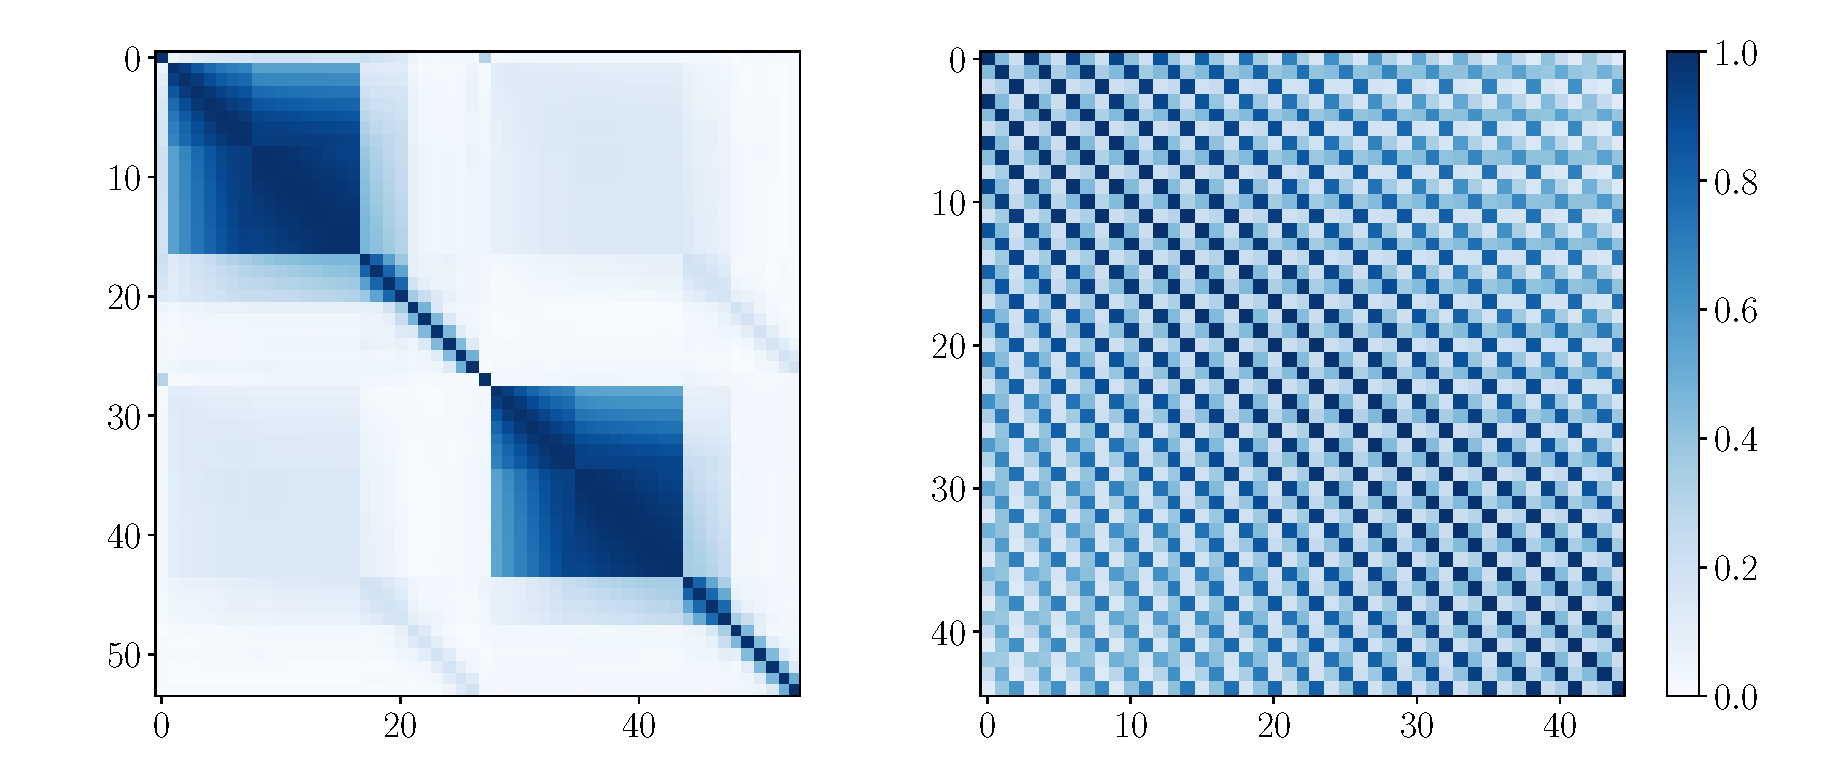
\includegraphics[width=\linewidth]{figs/ch3/corr_matrix}
	\caption{Матрицы корреляций для матрицы плана~$\bX$ и целевой матрицы~$\bY$ для данных ECoG}
	\label{ch3:fig:corr_matrix}
\end{figure}

\textbf{Результаты.}
Применим метод SymImp QPFS для различных значений коэффициента~$\alpha_3$ согласно формуле~\eqref{ch3:eq:alphas3}.
Зависимость значимостей целевых векторов~$\bz_y$ относительно коэффициента~$\alpha_3$ для различных значений~$k$ показана на Рис.~\ref{ch3:fig:features_vs_alpha_ecog}.
Значимости целевых векторов почти одинаковы для всех координат запястья при прогнозировании одного отсчёта времени ($k = 1$), 
что отражает независимость между координатами $x$, $y$ и $z$.
Для $k = 2$ и $k = 3$ значимости некоторых целевых векторов становятся нулевыми при увеличении~$\alpha_3$.
Вертикальные линии соответствуют оптимальному значению~$\alpha_3$, вычисленному по~\eqref{ch3:eq:alpha_3}. 
При этом значении $\alpha_3$ значимости компонент~$\bz_y$ совпадают. 
Таким образом, метод не учитывает различия между целевыми векторами для $k=1, 2, 3$.

Предлагаемые методы QPFS для случая векторной целевой переменной, приведенные в таблице~\ref{ch3:tbl:summary} применяются для набора данных ECoG. 
Решим задачу выбора признаков для каждого из методов, чтобы получить вектора значимостей признаков. 
Отсортируем по убыванию признаки по значению их значимостей. Обучим линейную модель, постепенно добавляя в неё признаки. 
Исследуются значения описанных критериев качества при увеличении количества отобранных признаков. 
На Рис.~\ref{ch3:fig:ecog_3_30_metrics} показаны результаты для случая прогнозирования $k = 30$ отсчётов времени. 
Порог значимости признаков~$\tau$ обозначен цветными тиками. 
Пороговые значения $\tau$ для предлагаемых методов больше, чем для базового метода RelAgg. 
Метод SymImp имеет большой порог, не позволяя получить малый набор признаков.
Однако метод SymImp обладает наилучшей предсказательной способностью с точки зрения sRMSE на тестовых данных.
Второй по качеству результат по sRMSE показал метод AsymImp.
Все предложенные методы достигают меньшей ошибки на тестовой выборке по сравнению с методом RelAgg. 
Критерий устойчивости также выше для предложенных методов.
Метод AsymImp показывает лучшие результаты с точки зрения качества прогнозирования и размера выбранного подмножества признаков.

\begin{figure}[ht]
	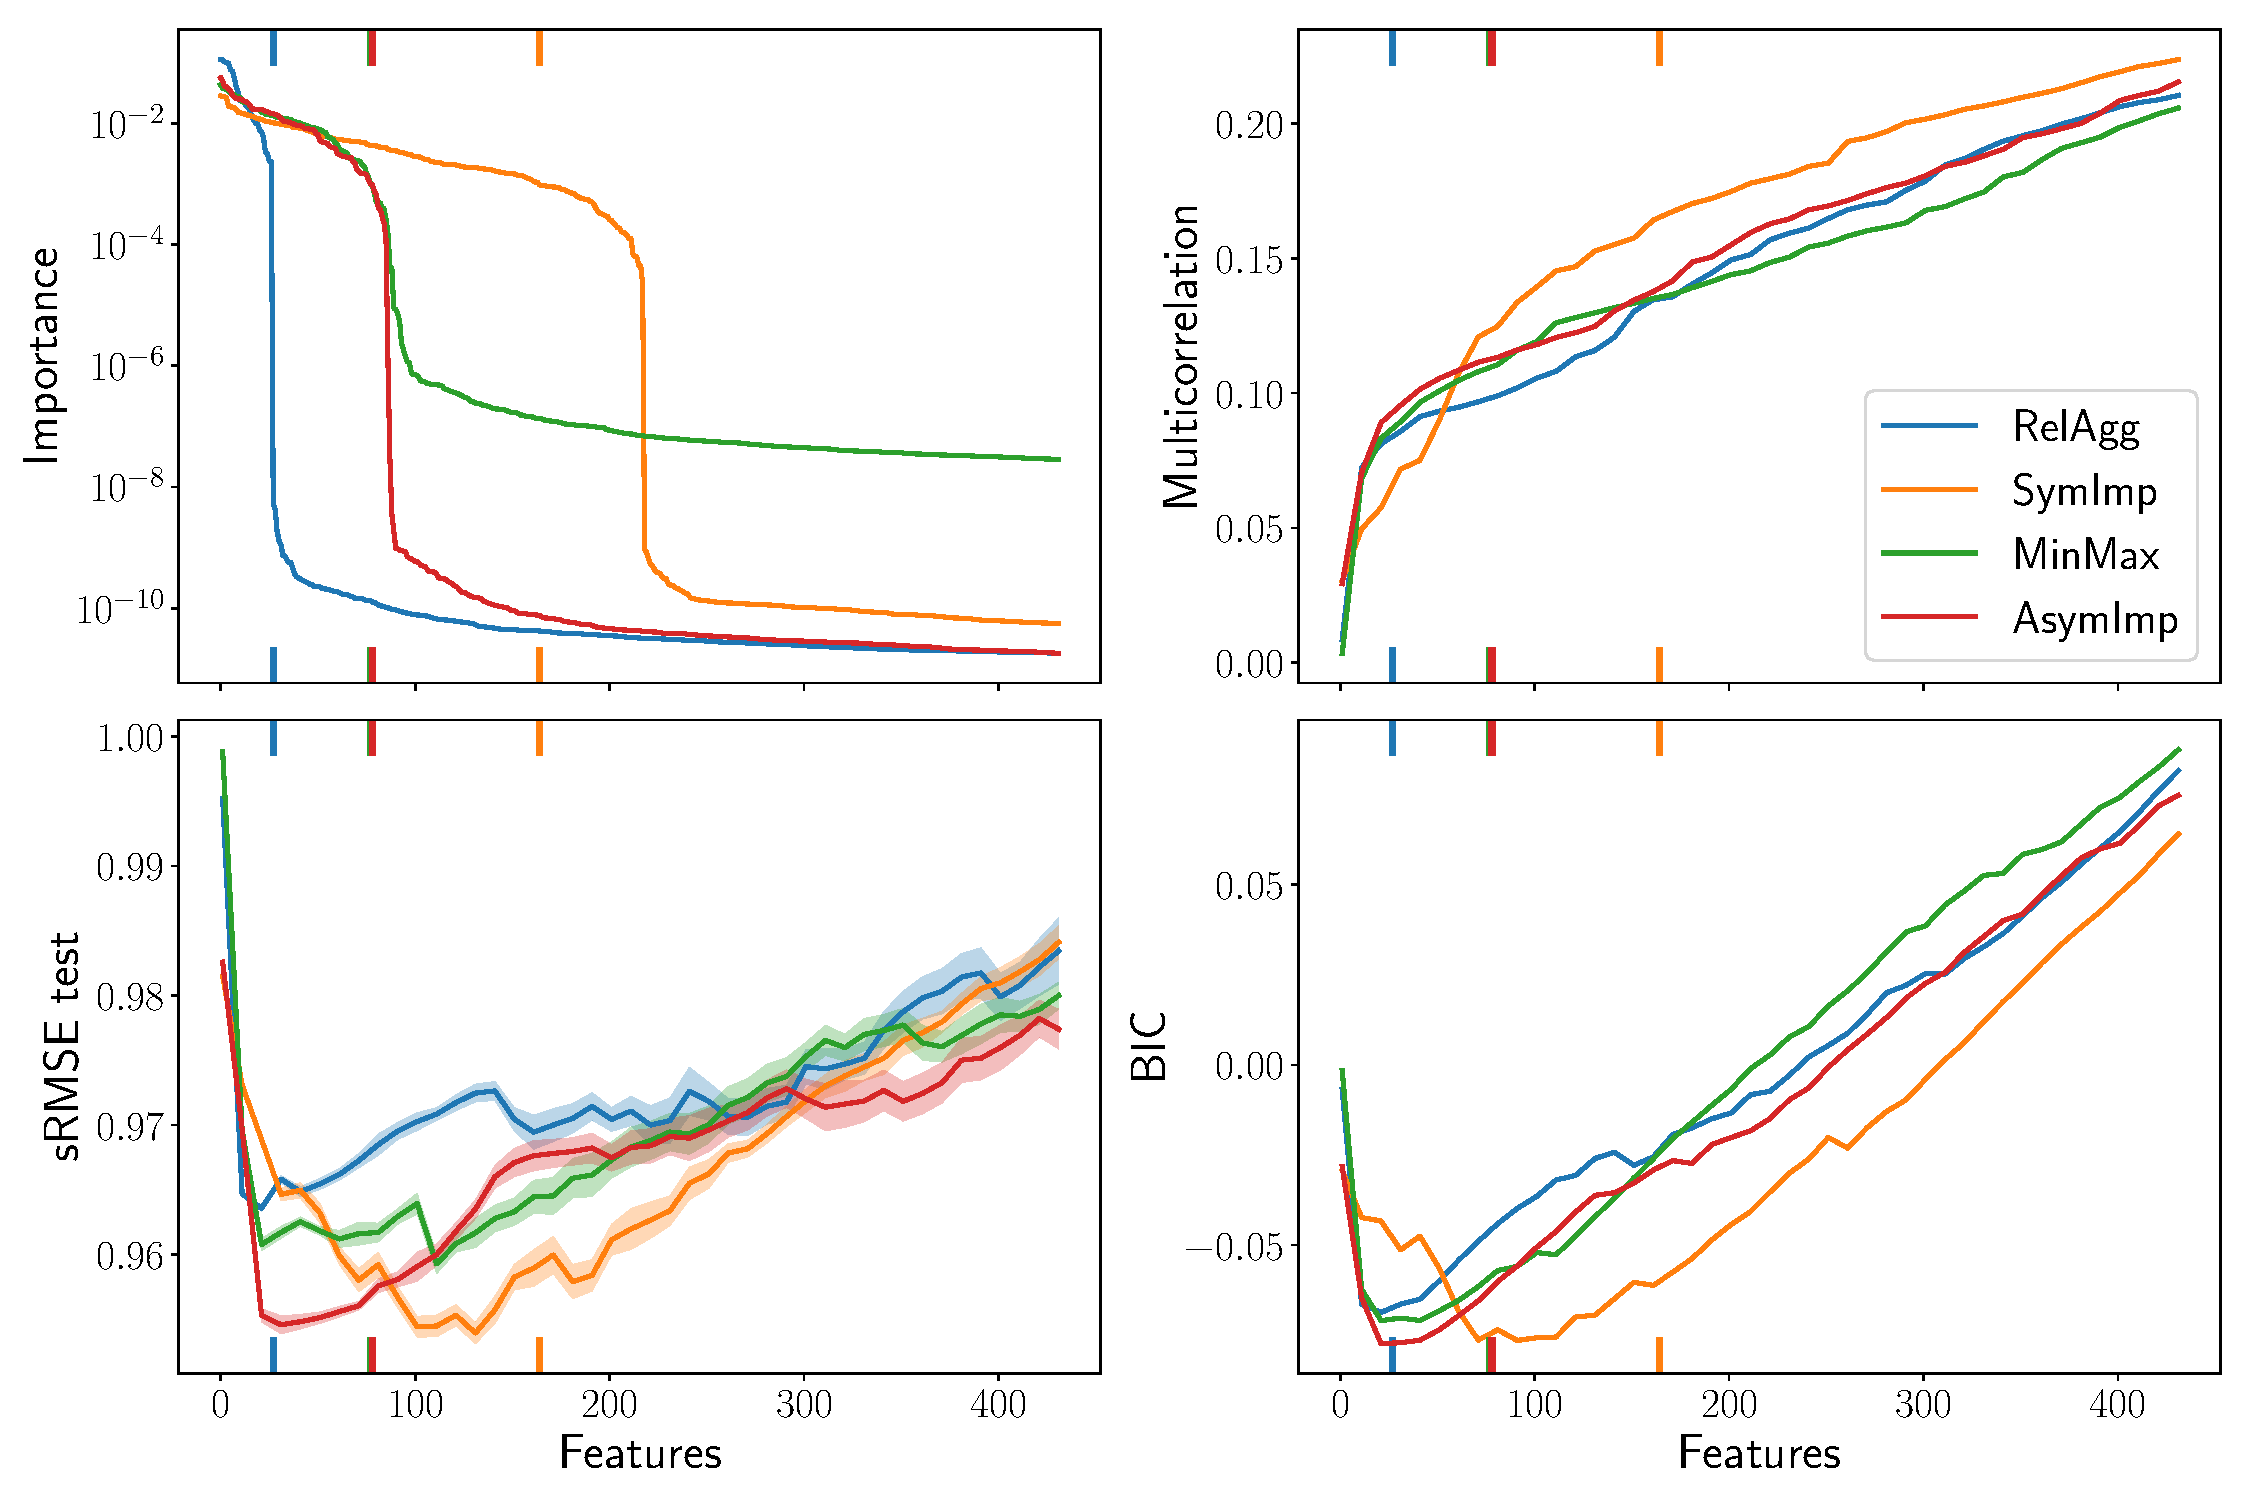
\includegraphics[width=\linewidth]{figs/ch3/ecog_3_30_metrics}
	\caption{Сравнение предложенных методов выбора признаков для данных ECoG при прогнозировании $k = 30$ отсчётов времени}
	\label{ch3:fig:ecog_3_30_metrics}
\end{figure}

Чтобы сравнить структуру выбранных подмножеств признаков и исследовать стабильность процедуры выбора признаков, используется метод генерации данных с помощью бутстрепа. 
Генерируется множество подвыборок, выбирая объекты по одному с возвращениями. 
Затем решается задача выбора признаков для каждой пары матрицы исходных объектов~$\bX$ и  матрицы целевых объектов~$\bY$.
Сравниваются полученные вектора значимостей для различных подвыборок данных. 
В качестве меры стабильности работы методов вычисляется средний попарный коэффициент корреляции Спирмена и попарное $\ell_2$ расстояние.
В таблице~\ref{ch3:tbl:stability} показана средняя ошибка sRMSE, размер подмножества признаков и описанные статистики для каждого метода. 
Ошибка считалась на обученной линейной модели с использованием $50$ признаков с наибольшими значениями значимостей.
Asymimp дает наименьшую ошибку на тестовой выборке. 
Размер выбранных подмножеств объектов завышен при использовании порогового значения~$\tau=10^{-4}$. 
Оптимальное значение~$\tau$ может быть подобрано с помощью процедуры кросс-валидации.

\begin{table}[ht]
	\caption{Стабильность предложенных методов выбора признаков}
	\centering
	\begin{tabular}{l|ccccc}
		\hline
		& sRMSE  & $\|\ba\|_0$ & Spearman $\rho$ & $\ell_2$ \\ \hline
		RelAgg & 0.965 $\pm$ 0.002 & 26.8 $\pm$ 3.8 & 0.915 $\pm$ 0.016 & 0.145 $\pm$ 0.018   \\
		SymImp & 0.961 $\pm$ 0.001 & 224.4 $\pm$ 9.0 & 0.910 $\pm$ 0.017 & 0.025 $\pm$ 0.002   \\
		MinMax & 0.961 $\pm$ 0.002 & 101.0 $\pm$ 2.1& 0.932 $\pm$ 0.009 & 0.059 $\pm$ 0.004   \\
		AsymImp & 0.955 $\pm$ 0.001 & 85.8 $\pm$ 10.2& 0.926 $\pm$ 0.011 & 0.078 $\pm$ 0.007  \\ \hline
	\end{tabular}
	\label{ch3:tbl:stability}
\end{table}

Для того, чтобы сравнить методы снижения размерности и выбора признаков, используется модель PLS, описанная в главе~\ref{ch:pls}. 
На Рис.~\ref{ch3:fig:pls_vs_k} показана ошибка sRMSE на тренировочной и тестовой выборках в зависимости от размерности скрытого пространства~$l$.
Ошибка на тестовой выборке достигает минимума при $l = 11$.
Метод PLS является более гибким подходом по сравнению с линейной моделью, построенной на подмножестве признаков, так как использует все исходные признаки.
Это приводит к меньшей ошибке, но модель не является разреженной.

На Рис.~\ref{ch3:fig:models} приведено сравнение 3 моделей: линейной регрессии; регрессии PLS, построенной на 100 признаках QPFS; регрессии PLS со всеми признаками.
Линейная регрессия со всеми признаками не рассматривается, так как ее результаты близки к константному прогнозу. На рисунке также приведены результаты методов lasso и elastic net, которые широко используются для выбора признаков.
В данном эксперименте использовался метод Asymimp QPFS.
Размерность скрытого пространства PLS $l = 15$.
Результаты регрессии PLS значительно лучше, линейной регрессии с признаками QPFS.
Это означает, что последняя модель не является достаточно гибкой.
Тем не менее, лучший результат показывает модель PLS, построенная на признаках QPFS. 
Данная модель является разреженной, так как использует только 100 исходных признаков.
Способность модели PLS находить оптимальное скрытое представление данных улучшает предсказательную способность модели.

\begin{figure}[ht]
	\begin{minipage}{.41\linewidth}
		\centering
		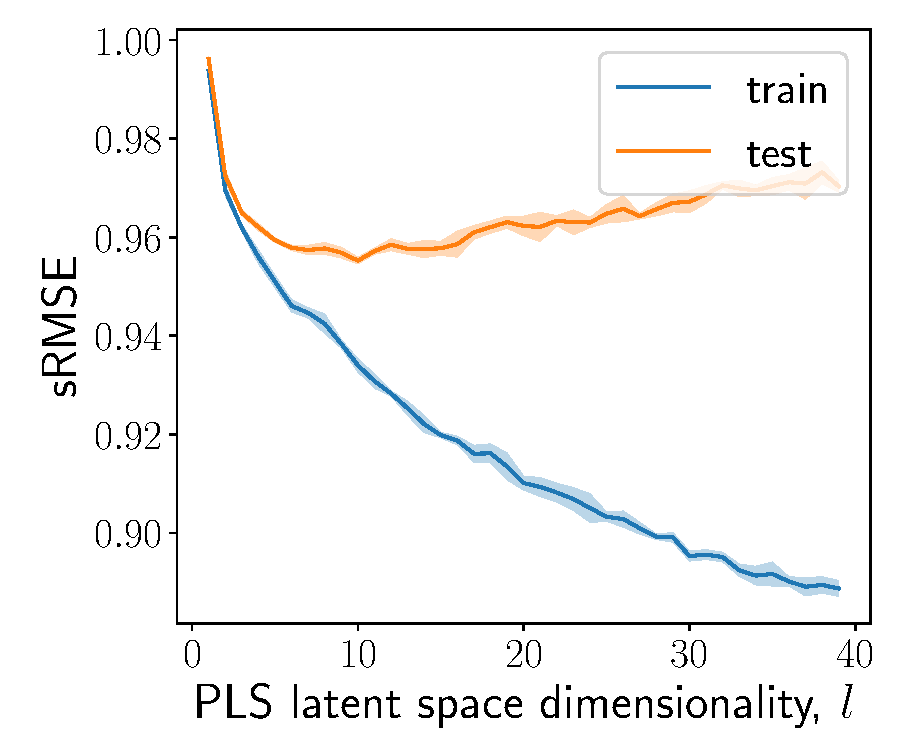
\includegraphics[width=1.\linewidth]{figs/ch3/pls_vs_k}
		\caption{ Ошибка sRMSE на тестовой выборке для модели PLS}
		\label{ch3:fig:pls_vs_k}
	\end{minipage}%
	\begin{minipage}{.55\linewidth}
		\centering
		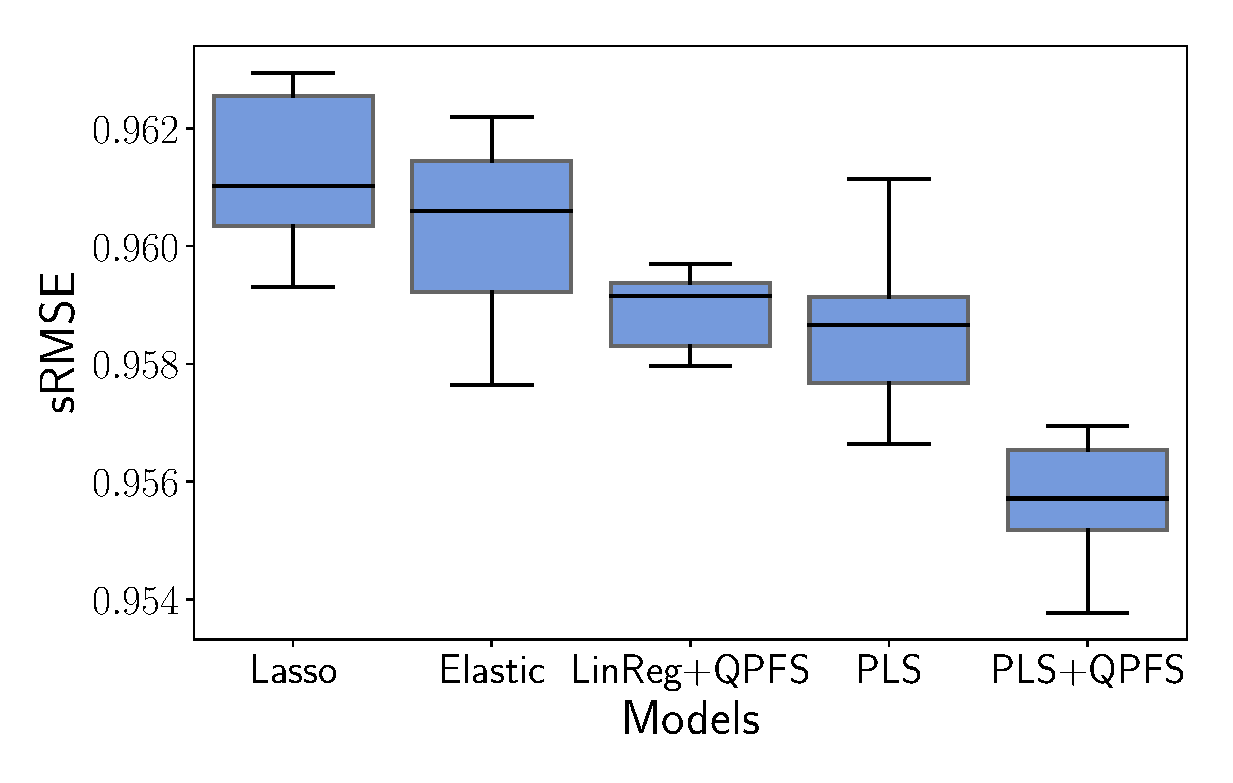
\includegraphics[width=1.\linewidth]{figs/ch3/models2}
		\caption{Диаграммы размаха значений sRMSE на тестовой выборке для моделей Lasso, Elastic, LinReg+QPFS, PLS, PLS+QPFS}
		\label{ch3:fig:models}
	\end{minipage}
\end{figure}

\textbf{Глава 4. Выбор параметров нелинейных моделей с помощью квадратичного отбора признаков}
\label{ch:newton_qpfs}

Функция ошибки для моделей с большим числом параметров имеет сложный ландшафт с многими локальными минимумами.
В этом случае алгоритм оптимизации приводит к разным решениям в зависимости от инициализации исходных параметров.

Алгоритм оптимизации представляет собой итерационный процесс.
На каждом шаге для получения следующего приближения параметров модели обновляются текущие параметры.
Разработано множество алгоритмов оптимизации первого порядка, использующих вектор первых производных функции ошибки.
Наиболее известными алгоритмами являются градиентный спуск, 
метод момента Нестерова~\cite{nesterov1983momentum}, AdaGrad~\cite{duchi2011adagrad}, Adam~\cite{kingma2014adam}.
Данные алгоритмы используются для оптимизации глубоких нейронных сетей~\cite{goodfellow2016deeplearningbook}.
Метод Ньютона~--- алгоритм второго порядка, использующий матрицу вторых производных функции ошибки.
Метод Ньютона находит обновления параметров для квадратичной аппроксимации функции ошибки и сходится за адекватное число итераций.
Недостатком методов оптимизации второго порядка является огромная и плохо обусловленная матрица Гессиана.
Процесс оптимизации в этом случае расходится и является вычислительно дорогостоящим.
Авторы~\cite{avriel2003nonlinear,blaschke1997convergence} предлагают аппроксимации для матрицы Гессиана и регуляризацию для решения этой проблемы.
В статье~\cite{botev2017newtondeeplearning} метод Ньютона применяется к глубоким нейронным сетям.

В данной главе приводится анализ параметров модели, которые не находятся в оптимуме.
Приводится метод выбора активных параметров модели, основанный на методе QPFS, который подробно описан в главе~\ref{ch:qpfs}.
Рассматриваются задачи нелинейной регрессии с квадратичной функцией потерь, логистической регрессии с кросс-энтропийной функцией потерь.  

%%%%%%%%%%%%%%%%%%%%%%%%%%%%%%%%%%%%%%%%%%%%%%%%
\textbf{Задача выбора параметров для оптимизации нелинейных моделей.}
\label{sec:ch4:newton_qpfs_param_selection}
%%%%%%%%%%%%%%%%%%%%%%%%%%%%%%%%%%%%%%%%%%%%%%%%

Модель $f( \bx, \btheta)$ с параметрами $\btheta \in \mathbb{R}^p$ предсказывает целевой объект~$y \in \bbY$ по исходному объекту~$\bx \in \bbR^{n}$. Пространство~$\bbY$ представляет собой бинарные метки классов~$\{0, 1\}$ для задачи двухклассовой классификации и~$\bbR$ для задачи регрессии.
Даны матрица исходных объектов~$\bX = [\bx_1, \dots, \bx_m]^{\T} \in \bbR^{m \times n}$ и целевой вектор~$\by = [y_1, \dots, y_m]^{\T} \in \bbY^{m}$. 
Цель состоит в нахождении оптимальных параметров~$\btheta^*$.
Параметры~$\btheta$ вычисляются минимизацией функции ошибки:
\begin{equation}
	\btheta^* = \argmin_{\btheta \in \bbR^p} \cL(\btheta, \bX, \by).
	\label{ch4:eq:error_function}
\end{equation}
Данная задача полностью соответствует рассмотренной задаче~\eqref{ch1:eq:loss_min_param} для случая скалярной целевой переменной ($r=1$).
В качестве функции ошибки~$\cL (\btheta, \bX, \by)$ рассматриваются квадратичная ошибка для задачи регрессии:
\begin{equation}
	\cL(\btheta, \bX, \by) = \frac 12 \| \by - \mathbf{f}(\bX, \btheta) \|_2^2 = \frac 12 \sum_{i=1}^m \bigl( y_i - f(\bx_i,  \btheta)\bigr)^2,
	\label{ch4:eq:squared_error}
\end{equation}
и функция кросс-энтропии для задачи бинарной классификации: 
\begin{equation}
	\cL(\btheta, \bX, \by) = \sum_{i=1}^m \bigl[y_i \log f (\bx_i , \btheta) + (1-y_i) \log \bigl(1 - f (\bx_i , \btheta)\bigr)\bigr].
	\label{ch4:eq:log_loss}
\end{equation}

Задача~\eqref{ch4:eq:error_function} решается с помощью итеративной процедуры оптимизации. 
Для получения параметров на шаге~$k$ текущие параметры $\btheta^{k-1}$ обновляются по следующему правилу:
\begin{equation}
	\btheta^k = \btheta^{k - 1} + \Delta \btheta^{k - 1}.
	\label{ch4:eq:update_rule}
\end{equation}
Авторы используют метод оптимизации Ньютона для выбора вектора обновлений~$\Delta \btheta$.

Метод Ньютона нестабилен и вычислительно сложен. 
В данной статье предлагается стабильный метод Ньютона. 
Перед шагом градиента предлагается выбрать подмножество активных параметров модели, которые оказывают наибольшее влияние на функцию ошибки~$\cL (\btheta, \bX, \by)$.
Введём определение активного параметра модели, используя необходимое условие оптимальности первого порядка.
\begin{definition}
	\label{ch4:def:active_param}
	Параметр $\theta_j$ для модели $f(\bx, \btheta)$ является \textit{активным}, если $\bJ^{\T} (\mathbf{f}(\bx, \btheta) - \by) \neq 0$.
\end{definition}
Подробный вывод условия из определения приводится в разделе~\ref{sec:ch4:newton_qpfs_algorithm}.
Обновление параметров производится только для отобранного множества индексов~$\cA = \bigl\{j: a_j = 1, \ba \in \{0, 1\}^p\bigr\}$
\begin{align*}
	\btheta_{\cA}^k &= \btheta_{\cA}^{k - 1} + \Delta \btheta_{\cA}^{k - 1}, \quad \btheta_{\cA} = \{\theta_j: j \in \cA \}, \\
	\btheta_{\bar{\cA}}^k &= \btheta_{\bar{\cA}}^{k - 1}, \quad \btheta_{\bar{\cA}} = \{\theta_j: j \notin \cA \}.
\end{align*}
Чтобы выбрать оптимальное подмножество индексов~$\cA$, из всех возможных $2^p - 1$~подмножеств, вводится функция ошибки
\begin{equation}
	\ba = \argmin_{\ba' \in \{0, 1\}^p} S(\ba', \bX, \by, \btheta),
	\label{ch4:eq:subset_selection}
\end{equation}
аналогичная функции ошибки~\eqref{ch3:eq:feature_selection} для задачи выбора признаков. 
Задача~\eqref{ch4:eq:subset_selection} решается на каждом шаге $k$ процесса оптимизации для текущих параметров~$\btheta^k$.

Метод QPFS используется для решения задачи~\eqref{ch4:eq:subset_selection}.
QPFS выбирает подмножество параметров~$\ba$ для вектора обновлений~$ \Delta \btheta$, которые оказывают наибольшее влияние на вектор остатков и являются попарно независимыми.
Функция ошибки~\eqref{ch3:eq:qpfs_problem} соответствует функции ошибки~$S(\ba, \bX, \by, \btheta)$
\begin{equation}
	\ba = \argmax_{\ba' \in \{1, 0\}^p} S(\ba', \bX, \by, \btheta) \Leftrightarrow \argmin_{\ba  \in \bbR^p_+, \, \|\ba\|_1=1} \bigl[\ba^{\T} \bQ \ba - \alpha \cdot \mathbf{b}^{\T} \ba \bigr].
\end{equation}
В работе показано, что для модели нелинейной регрессии с квадратичной функцией ошибки~\eqref{ch4:eq:squared_error} и для модели логистической регрессии с кросс-энтропией~\eqref{ch4:eq:log_loss}, каждый шаг оптимизации эквивалентен задаче линейной регрессии~\eqref{ch3:eq:linear_regression}.

%%%%%%%%%%%%%%%%%%%%%%%%%%%%%%%%%%%%%%%%%%%%%%%%
\textbf{Метод Ньютона для оптимизации параметров.}
\label{sec:ch4:newton_algorithm}
%%%%%%%%%%%%%%%%%%%%%%%%%%%%%%%%%%%%%%%%%%%%%%%%

Метод Ньютона использует условие оптимизации первого порядка для задачи~\eqref{ch4:eq:error_function} и линеаризует градиент $S (\btheta)$
\[
	\nabla S (\btheta + \Delta \btheta) = \nabla S(\btheta) + \bH \cdot \Delta \btheta = 0,
\]
\[
	\Delta \btheta = - \bH^{-1} \nabla S(\btheta).
\]
где $\bH = \nabla^2 S(\btheta)$ является матрицой Гессиана функции ошибки $S(\btheta)$.

Итерация~\eqref{ch4:eq:update_rule} метода Ньютона имеет вид
\[
	\btheta^k = \btheta^{k-1} - \bH^{-1} \nabla S(\btheta).
\]
На каждой итерации требуется обращать матрицу Гессиана $\bH$.
Мерой плохой обусловленности для матрицы Гессиана~$\bH$ является число обусловленности
\[
	\kappa(\bH) = \frac{\lambda_{\text{max}}(\bH)}{\lambda_{\text{min}}(\bH)},
\]
где $\lambda_{\text{max}}(\bH), \lambda_{\text{min}}(\bH)$ являются максимальным и минимальным собственными значениями~$\bH$. Большое число обусловленности~$\kappa (\bH)$ приводит к нестабильности процесса оптимизации.
Предложенный метод уменьшает размер матрицы Гессиана~$\bH$. Согласно экспериментам, приведенным в разделе~\ref{sec:ch4:newton_qpfs_exp} предлагаемый метод приводит к меньшему числу обусловленности~$\kappa (\bH)$.

Размер шага метода Ньютона может быть чрезмерно большим. Для контроля размера шага обновлений добавим параметр $\eta$ в правило обновления~\eqref{ch4:eq:update_rule}
\[
	\btheta^k = \btheta^{k - 1} + \eta \Delta \btheta^{k - 1}, \quad \eta \in [0, 1].
\]

Для выбора соответствующего размера шага~$\eta$ используется правило Армихо~\cite{armijo1966minimization}. Выбирается максимальное~$\eta$ так, чтобы выполнялось условие
\[
	S(\btheta^{k - 1} + \eta \Delta \btheta^{k - 1}) < S(\btheta^{k - 1}) + \gamma \eta \nabla S^{\T}(\btheta^{k-1})\btheta^{k - 1}, \quad \gamma \in [0, 0.5].
\]

\textbf{Модель нелинейной регрессии.}
Предположим, что модель $f (\bx , \btheta)$ близка к линейной в окрестности точки $\btheta + \Delta \btheta$
\[
	\mathbf{f}(\bX , \btheta + \Delta \btheta) \approx \mathbf{f}(\bX , \btheta) + \bJ \cdot \Delta  \btheta,
\]
где $\mathbf{J} \in \bbR^{m \times p}$ является матрицой Якоби
\begin{equation*}
	\bJ = 
	\begin{pmatrix}
		\frac{\partial f(\bx_1 , \btheta)}{\partial \theta_1} & \dots & 
		\frac{\partial f(\bx_1 , \btheta)}{\partial \theta_p} \\
		\dots & \dots & \dots \\
		\frac{\partial f(\bx_m , \btheta)}{\partial \theta_1} & \dots & 
		\frac{\partial f(\bx_m , \btheta)}{\partial \theta_p}
	\end{pmatrix}.
\end{equation*}
В соответствии с этим предположением градиент~$\nabla S(\btheta)$ и Гессиан матрицы~$\bH$ функции ошибки~\eqref{ch4:eq:squared_error} равняются
\begin{equation}
	\nabla S(\btheta) = \bJ^{\T} (\by - \mathbf{f}), \quad \bH = \bJ^{\T} \bJ.
	\label{ch4:eq:nonlin_reg_deriv}
\end{equation}
Данные предположения приводят к методу Гаусса-Ньютона и правилу обновления~\eqref{ch4:eq:update_rule}
\[
	\btheta^k = \btheta^{k - 1} + (\bJ^{\T} \bJ)^{-1}\bJ^{\T}(\mathbf{f} - \by).
\]
Вектор обновления~$\Delta \btheta$ является решением задачи линейной регрессии
\begin{equation}
	\| \be - \bF \Delta \btheta \|_2^2 \rightarrow \min_{\Delta \btheta \in \bbR^{p}},
	\label{ch4:eq:lin_reg_nonlin_reg}
\end{equation}
где $\be = \mathbf{f} - \by$ и $\bF = \bJ$.

В качестве нелинейной модели рассматривается модель двухслойной нейронной сети. В этом случае модель~$f (\bx, \btheta)$ принимает вид:
\[
	f(\bx, \btheta) = \sigma(\bx^{\T} \bW_1) \bw_2.
\]
Здесь~$\bW_1 \in \bbR^{m \times h}$~--- матрица параметров, которые соединяют исходные признаки с $h$ скрытыми нейронами. Функция нелинейности $\sigma(\cdot)$ применяется поэлементно. Параметры~$\bw_2 \in \bbR^{h \times 1}$ соединяют скрытые нейроны с выходом. 
Вектор параметров модели~$\btheta$ представляет собой объединение векторизованных матриц~$\bW_1$, $\bw_2$.

\textbf{Модель логистической регрессии.}
Для логистической регрессии модель имеет вид $f(\bx , \btheta) = \sigma(\bx^{\T} \btheta)$ с сигмоидной функцией активации~$\sigma(\cdot)$.
Градиент и Гессиан функции ошибки~\eqref{ch4:eq:log_loss} равны
\begin{equation}
	\nabla S(\btheta) = \bX^{\T} (\mathbf{f} - \by), \quad \bH = \bX^{\T} \bR \bX,
	\label{ch4:eq:log_reg_deriv}
\end{equation}
где $\bR$~--- это диагональная матрица с диагональными элементами $f(\bx_i , \btheta) \cdot (1 - f(\bx_i , \btheta))$.

Правило обновления~\eqref{ch4:eq:update_rule} в этом случае принимает вид
\[
	\btheta^k = \btheta^{k - 1} + (\bX^{\T} \bR \bX)^{-1} \bX^{\T} (\by - \mathbf{f}).
\]
Этот алгоритм известен как итеративный алгоритм взвешенных наименьших квадратов (IRLS)~\cite{holland1977robust}. Вектор обновлений $\Delta \btheta$ является решением задачи линейной регрессии
\begin{equation}
	\| \be - \bF \Delta \btheta \|_2^2 \rightarrow \min_{\Delta \btheta \in \bbR^{p}},
	\label{ch4:eq:lin_reg_log_reg}
\end{equation}
где $\be = \bR^{-1/2} (\by - \mathbf{f})$ и $\bF = \bR^{1/2}\bX$.

%%%%%%%%%%%%%%%%%%%%%%%%%%%%%%%%%%%%%%%%%%%%%%%%
\section{Метод Ньютона с выбором параметров с помощью квадратичного программирования}
\label{sec:ch4:newton_qpfs_algorithm}
%%%%%%%%%%%%%%%%%%%%%%%%%%%%%%%%%%%%%%%%%%%%%%%%

Предлагается адаптировать метод QPFS для решения задач~\eqref{ch4:eq:lin_reg_nonlin_reg} и \eqref{ch4:eq:lin_reg_log_reg}. 
Матрица парных взаимодействий~$\bQ$ и вектор релевантностей~$\bb$ имеют вид
\[
	\bQ = \text{Sim} (\bF), \quad \bb = \text{Rel} (\bF, \be).
\]

Выборочный коэффициент корреляции равен нулю для ортогональных векторов.
Покажем, что в оптимальной точке~$\btheta^*$ вектор~$\be$ ортогонален столбцам матрицы~$\bF$. 
В этом случае вектор~$\bb = \text{Rel} (\bF, \be)$ равен нулю. Это означает, что член, учитывающий релевантность, в данном случае исключается.
Условие оптимальности первого порядка гарантирует это свойство для модели нелинейной регрессии
\[
	\bF^{\T} \be = \bJ^{\T} (\mathbf{f} - \by) = - \nabla S(\btheta^*) = \boldsymbol{0},
\]
и для модели логистической регрессии
\[
	\bF^{\T} \be = \bX \bR^{-1/2} \bR^{1/2} (\by - \mathbf{f}) = \bX^{\T} (\by - \mathbf{f}) = \nabla S(\btheta^*) = \boldsymbol{0}.
\]
Данное условие используется в качестве индикатора активности параметра модели в определении~\ref{ch4:def:active_param}.
Псевдокод предлагаемого алгоритма приведён в алгоритме~\ref{ch4:alg:QPFSNewton}.

\begin{algorithm}[ht]
	\caption{QPFS + Ньютон алгоритм}
	\label{ch4:alg:QPFSNewton}
	\begin{algorithmic}
		\REQUIRE $\varepsilon$~--- допустимое отклонение;\\
		\hspace{1.07cm}$\tau$~-- пороговое значение;\\
		\hspace{1.07cm}$\gamma$~--- параметр правила Армихо.
		\ENSURE $\btheta^*$;
		\STATE  инициализировать $\btheta^0$;
		\STATE $k := 1$;
		\REPEAT
		\STATE вычислить $\be$ и $\bF$ для~\eqref{ch4:eq:lin_reg_nonlin_reg} или~\eqref{ch4:eq:lin_reg_log_reg} ;
		\vspace{0.1cm}
		\STATE $\bQ := \text{Sim} (\bF)$, $\bb := \text{Rel}(\bF, \be)$, $\alpha = \frac{\overline{\bQ}}{\overline{\bQ} + \overline{\bb}}$;
		\vspace{0.1cm}
		\STATE $\ba := \argmin_{\ba \geq 0, \, \|\ba\|_1=1}\ba^{\T} \bQ \ba - \alpha \cdot \mathbf{b}^{\T} \ba$;
		\vspace{0.1cm}
		\STATE $\cA := \{j: a_j = 1\}$;
		\vspace{0.1cm}
		\STATE вычислить $\nabla S(\btheta^{k-1})$, $\bH$ для \eqref{ch4:eq:nonlin_reg_deriv} или \eqref{ch4:eq:log_reg_deriv};
		\vspace{0.1cm}
		\STATE $\Delta \btheta^{k-1} = - \bH^{-1} \nabla S(\btheta^{k-1})$;
		\vspace{0.1cm}
		\STATE $\eta := \text{ArmijoRule}(\btheta^{k-1}, \gamma)$;
		\vspace{0.1cm}
		\STATE $\btheta_{\cA}^k = \btheta_{\cA}^{k - 1} + \eta \Delta \btheta_{\cA}^{k - 1}$;
		\vspace{0.1cm}
		\STATE $k := k + 1$;
		\vspace{0.1cm}
		\UNTIL{$\frac{\| \btheta^k - \btheta^{k-1} \|}{\| \btheta^k \|} < \varepsilon$}
	\end{algorithmic}
\end{algorithm}

%%%%%%%%%%%%%%%%%%%%%%%%%%%%%%%%%%%%%%%%%%%%%%%%
\textbf{Анализ значимостей параметров нелинейных моделей.}
\label{sec:ch4:newton_qpfs_exp}
%%%%%%%%%%%%%%%%%%%%%%%%%%%%%%%%%%%%%%%%%%%%%%%%

Целью вычислительного эксперимента является исследование свойств предложенного метода и сравнение его с другими методами. 

Исследована зависимость параметров метода QPFS для задачи нелинейной регрессии~\eqref{ch4:eq:lin_reg_nonlin_reg} и задачи логистической регрессии~\eqref{ch4:eq:lin_reg_log_reg}. 
Предположим, что вектор параметров~$\btheta^0$ лежит вблизи оптимального вектора параметров~$\btheta^*$. 
Рассмотрим отрезок
\[
	\btheta_{\beta} = \beta \btheta^* + (1 - \beta) \btheta^0; \quad \beta \in [0, 1] .
\]

Сгенерируем синтетический набор данных с 300 объектами и 7 признаками для задачи логистической регрессии. 
Ландшафт функции ошибки~\eqref{ch4:eq:log_loss} на сетке двух случайно выбранных параметров показан на Рис.~\ref{ch4:fig:log_reg_error}.
Поверхность функции ошибки выпуклая с вытянутыми линиями уровня вдоль некоторых параметров модели.
Добавим случайный шум к оптимальным параметрам~$\btheta^*$, чтобы получить точку~$\btheta^0$. Поведение вектора~$\bb$ на отрезке между~$\btheta^0$ и~$\btheta^*$ показано на Рис.~\ref{ch4:fig:log_reg_b_wrt_beta}.
Компоненты~$\bb$ начинают резко уменьшаться по мере приближения к оптимальной точке $\btheta^*$.

Для модели нелинейной регрессии используется классический набор данных Boston Housing с 506 объектами и 13 признаками.
Для простоты нейронная сеть содержит два скрытых нейрона.
Ландшафт функции ошибок для модели нейронной сети является более сложным. 
Функция ошибки не является выпуклой и содержит множество локальных минимумов.
Двумерный ландшафт функции ошибок для этого набора данных показан на Рис.~\ref{ch4:fig:neural_error}. 
Сетка строится для двух случайных параметров из матрицы~$\bW_1$.
Аналогично на Рис.~\ref{ch4:fig:neural_b_wrt_beta} показано, как изменяется вектор~$\bb$ при движении от точки~$\btheta^0$ до точки~$\btheta^*$. 
Компоненты вектора $\bb$ становятся близки к нулю вблизи оптимума. 
При достижении оптимального значения различные параметры влияют на остатки модели~$\be$.

На Рис.~\ref{ch4:fig:irls_qpfs_2d} показан процесс оптимизации для предложенного метода в случае логистической регрессии с двумя параметрами модели. 
Даже для двумерной задачи решение метода Ньютона нестабильно и число обусловленности $\kappa(\bH)$ матрицы Гессиана~$\bH$ может быть чрезвычайно большим. 
На каждом шаге алгоритма метод QPFS выбирает активные параметры для оптимизации. 
В данном примере предложенный метод выбирает и обновляет только один параметр на каждой итерации на первых шагах. 
Это делает метод более устойчивым.

На Рис.~\ref{ch4:fig:active_params_wrt_iters} показаны наборы активных параметров на итерациях для набора данных Boston Housing и нейронной сети с двумя скрытыми нейронами. 
Темные ячейки соответствуют активным параметрам, которые мы оптимизируем.

В рассмотренных примерах число обусловленности~$\kappa(\bH)$ для метода Ньютона на некоторых итерациях было чрезвычайно большим. 
Выбор активных параметров позволил значительно сократить число обусловленности. 

Приведём сравнение предложенного метода с существующими методами, а именно градиентным спуском~(GD), моментом Нестерова~\cite{nesterov1983momentum}, Adam~\cite{kingma2014adam} и оригинальным методом Ньютона. 
Проведены эксперименты для моделей нелинейной и логистической регрессий. 
Наборы данных были выбраны из репозитория UCI~\cite{uci2017}. 
Результаты показаны в таблицах~\ref{ch4:tbl:nonlin_reg_results} и \ref{ch4:tbl:log_reg_results}. 
Для каждого набора данных две строки таблиц содержат ошибки для тренировочной~(первая строка) и тестовой~(вторая строка) выборок. 
В таблице~\ref{ch4:tbl:nonlin_reg_results} приведена квадратичная ошибка, в таблице~\ref{ch4:tbl:log_reg_results}~--- кросс-энтропия.
Чтобы найти среднюю ошибку и ее стандартное отклонение использовалась процедура кросс валидации с разбиением на 5 фолдов. 
Предложенный метод показывает меньшую ошибку на трех из четырех наборов данных для нелинейной регрессии и на двух из трех наборов данных для логистической регрессии.

\begin{table}[h]
\footnotesize
	\caption{Средняя квадратичная ошибка рассматриваемых алгоритмов оптимизации для модели нелинейной регрессии}
	\label{ch4:tbl:nonlin_reg_results}
	\centering
	\begin{tabular}{|l|c|c|c|c|c|c|}
		\hline
		Выборка & \begin{tabular}[c]{@{}c@{}}\ $m$ \\ \ $n$ \end{tabular} 
		& GD 
		& Нестеров 
		& ADAM 
		& Ньютон 
		&
		\begin{tabular}[c]{@{}c@{}}QPFS+Ньютон\\ \end{tabular} \\ 
		\hline
		Boston House
		& 506
		& $27.2\pm4.6$
		& $46.0\pm11.0$
		& $35.4\pm2.5$           
		& $22.1\pm15.2$            
		& $20.9\pm10.4$   \\  
		Prices
		&\multicolumn{1}{c|}{13}
		& \multicolumn{1}{c|}{$32.4\pm5.6$}
		& \multicolumn{1}{c|}{$53.3\pm11.5$}
		& \multicolumn{1}{c|}{$37.8\pm7.0$}
		& \multicolumn{1}{c|}{$28.9\pm13.6$}
		& \multicolumn{1}{c|}{$\mathbf{24.5\pm9.4}$}\\ 
		\hline
		Communities
		& 1994
		& $48.0\pm6.4$
		& $31.4\pm2.8$
		& $23.3\pm3.7$        
		& $18.3\pm3.4$          
		&  $26.7\pm3.1$  \\ 
		and Crime
		&\multicolumn{1}{c|}{99}
		& \multicolumn{1}{c|}{$47,5\pm6.5$}
		& \multicolumn{1}{c|}{$32.9\pm4.3$}
		& \multicolumn{1}{c|}{$28,1\pm4.5$}
		& \multicolumn{1}{c|}{$28.8\pm3.6$}
		& \multicolumn{1}{c|}{$\mathbf{28.4\pm3.0}$} \\ 
		\hline
		Forest
		& 517
		& $18.9\pm0.4$
		& $1.83\pm0.4$
		& $1.81\pm0.6$             
		& $17.7\pm0.4$             
		& $17.9\pm0.4$   \\ 
		Fires
		&\multicolumn{1}{c|}{10}
		& \multicolumn{1}{c|}{$\mathbf{20.0\pm2.1}$}
		& \multicolumn{1}{c|}{ $20.2\pm2.2$}
		& \multicolumn{1}{c|}{ $\mathbf{20.0\pm2.0}$}
		& \multicolumn{1}{c|}{ $20.6\pm1.4$}
		& \multicolumn{1}{c|}{ $20.2\pm2.2$} \\ 
		\hline
		Residential
		& 372
		&  $51.6\pm17.7$
		&  $32.6\pm19.5$
		&  $30.0\pm24.8$            
		&  $35.5\pm24.7$            
		&   $30.3\pm10.7$ \\ 
		Building
		&\multicolumn{1}{c|}{103}
		& \multicolumn{1}{c|}{ $53.7\pm13.9$}
		& \multicolumn{1}{c|}{ $34.1\pm13.6$}
		& \multicolumn{1}{c|}{ $34.1\pm19.4$}
		& \multicolumn{1}{c|}{ $35.0\pm15.6$}
		& \multicolumn{1}{c|}{ $\mathbf{30.9\pm5.3}$} \\ 
		\hline
	\end{tabular}
\end{table}

\begin{table}[h]
\footnotesize
	\caption{Среднее значение кросс-энтропии рассматриваемых алгоритмов оптимизации для модели логистической регрессии}
	\label{ch4:tbl:log_reg_results}
	\centering
	\begin{tabular}{|l|c|c|c|c|c|c|}
		\hline
		Выборка & \begin{tabular}[c]{@{}c@{}}\ $m$ \\ \ $n$ \end{tabular} 
		& GD 
		& Нестеров 
		& ADAM 
		& Ньютон 
		&
		\begin{tabular}[c]{@{}c@{}}QPFS+Ньютон\\ \end{tabular} \\ 
		\hline
		Breast
		& 569
		& $0.6\pm0.1$
		& $0.4\pm0.1$
		& $0.8\pm0.2$           
		& $0.3\pm0.1$            
		& $0.2\pm0.1$   \\  
		Cancer
		&\multicolumn{1}{c|}{30}
		& \multicolumn{1}{c|}{$\mathbf{0.9\pm0.2}$}
		& \multicolumn{1}{c|}{$1.0\pm0.7$}
		& \multicolumn{1}{c|}{$1.2\pm0.2$}
		& \multicolumn{1}{c|}{$1.0\pm0.2$}
		& \multicolumn{1}{c|}{$1.1\pm0.3$}\\ 
		\hline
		Cardiotocography
		& 2126
		& $11.5\pm4.7$
		& $11.5\pm4.7$
		& $8.8\pm4.4$        
		& $11.5\pm5.7$          
		&  $7.7\pm4.2$  \\
		
		&\multicolumn{1}{c|}{21}
		& \multicolumn{1}{c|}{$11.6\pm5.8$}
		& \multicolumn{1}{c|}{$11.5\pm5.7$}
		& \multicolumn{1}{c|}{$9.0\pm2.6$}
		& \multicolumn{1}{c|}{$11.5\pm4.7$}
		& \multicolumn{1}{c|}{$\mathbf{7.7\pm4.7}$} \\ 
		\hline
		Climate Model
		& 540
		& $1.2\pm0.1$
		& $1.0\pm0.2$
		& $1.5\pm0.2$             
		& $1.0\pm0.5$             
		& $0.8\pm0.3$   \\ 
		Simulation Crashes
		&\multicolumn{1}{c|}{18}
		& \multicolumn{1}{c|}{$1.4\pm2.0$}
		& \multicolumn{1}{c|}{ $1.3\pm0.7$}
		& \multicolumn{1}{c|}{ $1.8\pm0.3$}
		& \multicolumn{1}{c|}{ $1.2\pm0.5$}
		& \multicolumn{1}{c|}{ $\mathbf{1.1\pm0.4}$} \\ 
		\hline
	\end{tabular}
\end{table}

\textbf{Глава 5. Метрические методы анализа временных рядов}
\label{ch:metric_learning}

При использовании в качестве функции ошибки модели квадратичной ошибки предполагается, что целевое пространство является евклидовым. 
Данное предположение не всегда является адекватным.
В данной главе ставится задача метрического обучения как поиск оптимальной метрики в целевом пространстве.
Рассматриваются задачи кластеризации и классификации множества временных рядов.

%%%%%%%%%%%%%%%%%%%%%%%%%%%%%%%%%%%%%%%%%%%%%%%%
\textbf{Метрическое обучение в задачах кластеризации временных рядов.}
\label{sec:ch5:metric_learning_clustering}
%%%%%%%%%%%%%%%%%%%%%%%%%%%%%%%%%%%%%%%%%%%%%%%%

Пусть~$\bX = [\bx_1, \dots, \bx_m]^{\T} \in \mathbb{R}^{m \times n}$~--- матрица плана.
Объект~$\bx_i = [x_i^1, \ldots, x_i^n]^{\T}$ задан в виде вектора в пространстве признаков.
Требуется выявить кластерную структуру данных и разбить множество объектов~$\bX$ на множество непересекающихся кластеров $\bbY = \{1, \dots, K\}$,
т.\,е.\ построить отображение $f: \bbR^n \to \bbY$.
Обозначим~$y_i = f (\bx_i)$, $y_i \in \bbY$~--- метка кластера объекта~$\bx_i$.
Необходимо выбрать метки кластеров~$\{y_i\}_{i=1}^m$ таким образом, чтобы расстояния между кластерами были максимальными.
Центроид~$\bmu$ множества объектов~$\bX$ и центроиды кластеров $\{\bmu_j\}_{j=1}^K$ вычисляются по формулам:
\begin{equation}
	\label{ch5:eq:mu}
	\boldsymbol{\mu} =\frac{1}{m} \sum_{i=1}^m\bx_i, \quad
	\boldsymbol{\mu}_j =\frac{ \sum_{i=1}^m [y_i = y_j]\bx_i } {\sum_{i=1}^m [y_i = y_j]}\,.
\end{equation}
Введем на множестве объектов~$\bX$ расстояние Махаланобиса
\begin{equation}
	d_{\bA} (\bx_i, \bx_j) = \sqrt{(\bx_i - \bx_j)^{\top} \bA^{-1} (\bx_i - \bx_j)},
	\label{ch5:eq:mahal_distance}
\end{equation}
где \textit{матрица трансформаций} $\mathbf{A} \in \bbR^{n \times n}$ является симметричной и неотрицательно определенной ($\mathbf{A}^{\T} = \mathbf{A}$, $\mathbf{A} \succeq 0$).
Зададим в качестве матрицы трансформации матрицу выборочной ковариации
\begin{equation}
	\label{ch5:eq:covMatrix}
	\bA = \frac{1}{m} \sum_{i=1}^m(\bx_i - \bmu)(\bx_i - \bmu)^{\T}.
\end{equation}
Функцией ошибки кластеризации назовем межкластерное расстояние:
\begin{equation}
	\cL \bigl(\{\bmu_j\}_{j=1}^K, \bX, \by\bigr)= - \sum_{j=1}^K N_j d_{\bA}^2(\bmu_j, \bmu),
	\label{ch5:eq:cluster_error_function}
\end{equation}
где $N_j = \sum_{i=1}^m [y_i = y_j]$~--- число объектов в кластере~$j$.

Поставим задачу кластеризации как задачу минимизации функции ошибки~\eqref{ch5:eq:cluster_error_function}
\begin{equation}
	\label{ch5:eq:Qmax}
	\cL \bigl(\{\boldsymbol{\mu}_j\}_{j=1}^K, \bX, \by \bigr) \to \min_{\boldsymbol{\mu}_j \in \bbR^{\T}}.
\end{equation}
Для решения этой задачи предлагается применить метод метрического обучения к матрице трансформации~$\bA$.
Найдем такую матрицу~$\bA$, для которой функционал качества принимает максимальное значение:
\begin{equation}
	\label{ch5:eq:Amax}
	\bA^* =\argmin_{\bA \in \bbR^{n \times n}} S \bigl(\{\bmu_j^*\}_{j=1}^K, \bX, \by \bigr)\,,
\end{equation}
где $\{\bmu_j^*\}_{j=1}^K$~--- решение задачи кластеризации~\eqref{ch5:eq:Qmax}.

%%%%%%%%%%%%%%%%%%%%%%%%%%%%%%%%%%%%%%%%%%%%%%%%
\textbf{Алгоритм адаптивного метрического обучения.}
\label{sec:ch5:metric_learning_adaptive}
%%%%%%%%%%%%%%%%%%%%%%%%%%%%%%%%%%%%%%%%%%%%%%%%

Для решения задач~\eqref{ch5:eq:Qmax}, \eqref{ch5:eq:Amax} используется алгоритм адаптивного метрического обучения.
Предлагается понизить размерность пространства объектов~$\bX$ с помощью линейного ортогонального преобразования~$\bP \in \bbR^{l \times n}$, $\bP^{\T} \bP = \mathbf{I}$, где новая размерность $l < n$
\[
	\bt_i = \bP \bx_i \in \bbR^l, \quad i = 1, \dots, m.
\]
Центроид~$\hat{\bmu}$ множества объектов~$\{\bt_i\}_{i=1}^m$ вычисляется по формуле~\eqref{ch5:eq:mu}. 
Расстояния между объектами вычисляются по формуле~\eqref{ch5:eq:mahal_distance}, где в качестве матрицы~$\hat{\mathbf{A}}$ используется матрица ковариаций~\eqref{ch5:eq:covMatrix} множества объектов $\{\hat{\bx}_i\}_{i=1}^m$
\[
	\hat{\mathbf{A}} =
	\frac{1}{m} \sum_{i=1}^m (\bt_i - \hat{\bmu})(\bt_i - \hat{\bmu})^{\T} =
	\frac{1}{m} \sum_{i=1}^m \bP(\bx_i - \bmu)(\bx_i - \bmu)^{\T} \bP^{\T} =  \bP \mathbf{A} \bP^{\T}.
\]
\begin{definition}
	Индикаторной матрицей назовем матрицу $\bY \in \bbR^{m \times K}$, где
	\[
	y_{ij} =
		\begin{cases}
			1, & \text{если $f(\bx_i) = y_j$;} \\
			0, & \text{если $f(\bx_i) \neq y_j$.}
		\end{cases}
	\]
\end{definition}
\begin{definition}
	Взвешенной индикаторной матрицей назовем матрицу
	$\mathbf{L} = \bY (\bY^{\T} \bY)^{-1/2} \in \bbR^{m \times K}$, элементы которой равны:
	\[
		l_{ij} =
		\begin{cases}
			\displaystyle    \frac{1}{\sqrt{N_j}}, & \text{если $f(\bx_i) = y_j$;} \\
			0, & \text{если $f(\bx_i) \neq y_j$.}
		\end{cases}
	\]
\end{definition}
В работе~\cite{ding2005equivalence} показано, что с использованием данных обозначений задача кластеризации~\eqref{ch5:eq:Qmax} и~задача метрического обучения~\eqref{ch5:eq:Amax} сводятся к общей задаче минимизации функции ошибки
\begin{multline}
	\cL = -\frac{1}{m} \text{trace} (\mathbf{L}^{\T} \bX^{\T} \bP^{\T} \hat{\mathbf{A}}^{-1} \bP \bX \mathbf{L}) = \\ = - \frac{1}{m} \text{trace} (\mathbf{L}^{\T} \bX^{\T} \bP^{\T}
	(\bP \mathbf{A} \bP^{\T})^{-1} \bP \bX \mathbf{L}) \to \min_{\bP, \mathbf{L}}.
	\label{ch5:eq:GLmax}
\end{multline}

Для решения задачи~\eqref{ch5:eq:GLmax} используется EM алгоритм.
На каждом шаге итеративно вычисляются текущие оптимальные значения матриц~$\bP$ и~$\mathbf{L}$.
На $E$-шаге необходимо найти матрицу~$\mathbf{L}$, которая является решением оптимизационной задачи~\eqref{ch5:eq:GLmax} при фиксированной матрице~$\bP$.
В качестве начального приближения получим взвешенную индикаторную матрицу~$\mathbf{L}$ с помощью алгоритма кластеризации $k$-средних с евклидовой метрикой.
На $M$-шаге производится нахождение оптимального значения матрицы~$\bP$ при фиксированной матрице~$\mathbf{L}$.
Алгоритм завершается при стабилизации функционала~$\cL$ на последовательности итераций.

\textbf{Алгоритм $k$-средних.}
В данной работе базовым алгоритмом для сравнения является алгоритм $k$-средних.
На первом шаге алгоритм выбирает из множества~$\bX$ случайным образом~$r$ объектов~$\{\bmu_j\}_{j=1}^K$~--- начальные центроиды кластеров.
Для каждого объекта~$\bx_i$ вычисляется расстояние~\eqref{ch5:eq:mahal_distance} до каждого центроида кластера~$\bmu_j$ с единичной матрицей трансформаций~$\mathbf{A}$.
Объект~$\bx_i$ относится к кластеру, расстояние до которого оказалось наименьшим.
Далее производится вычисление новых центроидов кластеров по формуле~\eqref{ch5:eq:mu}.
Алгоритм завершается, если значения центроидов кластеров стабилизируются.

\textbf{Оптимизация матрицы P с фиксированной матрицей L.}
Для любых двух квадратных матриц~$\mathbf{A}$ и~$\mathbf{B}$ справедливо $\text{trace}(\mathbf{AB}) = \text{trace}(\mathbf{BA})$.
Данное свойство позволяет переформулировать задачу~\eqref{ch5:eq:GLmax} следующим образом:
\[
	\cL = -\frac{1}{m} \text{trace} (\mathbf{L}^{\T} \bX^{\T} \bP^{\T} (\bP \mathbf{A} \bP^{\T})^{-1} \bP \bX \mathbf{L}) = -\frac{1}{m} \text{trace} \bigl((\bP \mathbf{A} \bP^{\T})^{-1} \bP \bX \mathbf{LL}^{T} \bX^{\T} \bP^{\T}\bigr).
\]
\begin{statement}
	Обозначим $\mathbf{B} = \bX \mathbf{LL}^{\T} \bX^{\T}$.
	Обозначим через $\bP = [\mathbf{v}_1, \ldots, \mathbf{v}_r]^{\bT}$ матрицу, состоящую из $r$ собственных векторов матрицы $\mathbf{A}^{-1}\mathbf{B}$, отвечающих наибольшим собственным значениям.
	Тогда решением~\eqref{ch5:eq:GLmax} является ортогональная матрица, полученная QR-разложением матрицы~$\bP^{\T}$.
\end{statement}
\begin{proof}
Функция ошибки~$\cL$~\ref{ch5:eq:cluster_error_function} зависит только от матрицы~$\bP$. Обозначим
\[
	s(\bP) = \text{trace} \bigl((\bP \mathbf{A} \bP^{\T})^{-1} \bP \mathbf{B} \bP^{\T}\bigr).
\]
На данном шаге задача~\eqref{ch5:eq:GLmax} принимает вид:
\begin{gather}
	\label{ch5:eq:Gmax}
	\bP^* = \argmax_{\bP \in \bbR^{l \times n}} s(\bP)\,; \\
	\label{ch5:eq:Gorth}
	\bP \bP^{\T} = \mathbf{I}\,.
\end{gather}
Ранг произведения матриц не превосходит рангов сомножителей, поэтому ранг матрицы~$\mathbf{B}$ не превосходит $K$.
Решением~\eqref{ch5:eq:Gmax} является матрица $\bP = [\mathbf{v}_1, \ldots, \mathbf{v}_K]^{\T}$, состоящая
из~$K$ собственных векторов матрицы $\mathbf{A}^{-1}\mathbf{B}$, отвечающих наибольшим собственным значениям.
Таким образом, размерность нового пространства объектов будет равна количеству кластеров $K$.

В общем случае матрица $\bP$ не является ортогональной.
Заметим, что для любой невырожденной матрицы $\bP$ верно $s(\bP) = s(\mathbf{M} \bP)$.
Для учета условия ортогональности~\eqref{ch5:eq:Gorth} найдем QR-разложение матрицы $\bP$.
Тогда ортогональная матрица $\bQ$ является оптимальным значением $\bP^*$.
\end{proof}

\textbf{Оптимизация матрицы L с фиксированной матрицей P.}
Обозначим $\hat{\mathbf{K}} = (1/N)\bX^{\T} \bP^{\T} \hat{\mathbf{A}}^{-1} \bP \bX$.
В работе~\cite{shawe2004kernel} показано, что тогда задача~\eqref{ch5:eq:GLmax} эквивалентна задаче кластеризации $k$-средних с заданным ядром $\hat{\mathbf{K}}$.

При фиксированной матрице $\bP$ задача~\eqref{ch5:eq:GLmax} принимает вид:
\begin{equation*}
	\text{trace} (\mathbf{L}^{\top} \hat{\mathbf{K}} \mathbf{L}) \to \max_{\mathbf{L} \in \bR^{m \times r}}.
\end{equation*}
Матрица $\hat{\mathbf{K}}$ является симметричной и неотрицательно определенной, тем самым может быть выбрана в качестве ядра.

%%%%%%%%%%%%%%%%%%%%%%%%%%%%%%%%%%%%%%%%%%%%%%%%
\textbf{Задача метрического обучения с динамическим выравниваем временных рядов.}
\label{sec:ch5:metric_learning_classification}
%%%%%%%%%%%%%%%%%%%%%%%%%%%%%%%%%%%%%%%%%%%%%%%%

Пусть объект $\mathbf{x}_i \in \mathbb{R}^n$~--- временной ряд, последовательность измерений некоторой исследуемой величины в различные моменты времени.
Пусть задана выборка $\{(\mathbf{x}_i, y_i)\}_{i=1}^m$~--- множество объектов с известными метками классов $y_i \in \bbY$, где $\bbY = \{1, \dots, K\}$~--- множество меток классов.

Требуется построить точную, простую, устойчивую модель классификации $a: \bbR^n \to \bbY$.
Данную модель представим в виде суперпозиции
\begin{equation*}
	a(\mathbf{x}) = b \circ \mathbf{f} \circ G\bigl(\mathbf{x}, \{\mathbf{c}_e\}_{e = 1} ^ K\bigr),
\end{equation*}
где $G$~--- процедура выравнивания временных рядов относительно центроидов классов~$\{\mathbf{c}_e\}_{e = 1} ^ K$, $\mathbf{f}$~--- алгоритм метрического обучения, $b$~--- алгоритм многоклассовой классификации.

\textbf{Выравнивание временных рядов.}
Для повышения качества и устойчивости алгоритма классификации предлагается провести выравнивание временных рядов каждого класса относительно центроида.

Пусть $\mathbf{X}_e$~--- множество объектов обучающей выборки, принадлежащих одному классу $e \in \bbY$.
Центроидом множества объектов $\mathbf{X}_e = \{\mathbf{x}_i|y_i=e\}_{i=1}^m$ по расстоянию $\rho$ назовем вектор $\mathbf{c}_e \in \mathbb{R}^n$ такой, что
\begin{equation}
	\label{ch5:eq:centroid_task}
	\mathbf{c}_e = \mathop{\text{argmin}}\limits_{{\mathbf{c} \in \mathbb{R}^n}}\sum_{\mathbf{x}_i \in \mathbf{X}_e}
	{\rho(\mathbf{x}_i ,\mathbf{c})}.
\end{equation}

Для нахождения центроида предлагается в качестве расстояния между временными рядами использовать путь наименьшей стоимости~\cite{berndt1994using,muller2007dynamic}, найденный методом динамической трансформации времени.
Псевдокод решения оптимизационной задачи~\eqref{ch5:eq:centroid_task} приведен в алгоритме~\ref{ch5:alg:DBA_pseudo}.
\begin{algorithm}[!t]
	\caption{Нахождение центроида $\text{DBA}(\mathbf{X}_e, \text{n\_iter})$}
	\label{ch5:alg:DBA_pseudo}
	\begin{algorithmic}[1]
		\REQUIRE $\mathbf{X}_e$~--- множество временных рядов, принадлежащих одному и тому же классу, n\_iter~--- количество итераций алгоритма.
		\ENSURE $\mathbf{c}$~--- центроид множества $\mathbf{X}_e$.
		
		\STATE {задать начальное приближение приближение центроида $\mathbf{c}$;}
		\FOR {$i = 1, \dots, \text{n\_iter}$}
		\FOR {$\mathbf{x} \in \mathbf{X}_e$}
		\STATE{вычислить выравнивающий путь между $\mathbf{c}$ и $\mathbf{x}$}
		\STATEx $ \quad \quad \text{alignment}(\mathbf{x}) := \text{DTWalignment}(\mathbf{c}, \mathbf{x})$;
		\ENDFOR
		\STATE {объединить поэлементно множества индексов для каждого отсчета времени}
		\STATEx {$ \quad \text{alignment} := \bigcup_{\mathbf{x} \in \mathbf{X}_e} \text{alignment}(\mathbf{x})$};
		\STATE {$\mathbf{c} = \text{mean}(\text{alignment})$}
		\ENDFOR
	\end{algorithmic}

	\textbf{DTWalignment}($\mathbf{c}$, $\mathbf{x}$)
	\begin{algorithmic}[1]
		\REQUIRE $\mathbf{c}, \mathbf{x}$~--- временные ряды.
		\ENSURE alignment~--- выравнивающий путь.\COMMENT {каждый индекс временного ряда~$\mathbf{x}$ поставлен в однозначное соответствие индексу временного ряда~$\mathbf{c}$}
		
		\STATE {построить $n \times n$-матрицу деформаций DTW}
		\STATEx {$\text{cost} := \text{DTW}(\mathbf{c}, \mathbf{x})$};
		
		\STATE {вычислить выравнивающий путь по матрице деформаций}
		\STATEx {$\text{alignment} := \text{DTWpath}(\text{cost})$};
	\end{algorithmic}
\end{algorithm}
Общая процедура выравнивания имеет следующий вид:
\begin{itemize}
	\item[1)]
	построить множество центроидов классов $\{\mathbf{c}_e\}_{e = 1}^K$;
	\item[2)]
	по множеству центроидов найти пути наименьшей стоимости между каждым
	временным рядом $\mathbf{x}_i$ и центроидом его класса $\mathbf{c}_{y_i}$;
	\item[3)]
	по каждому пути восстановить выравненный временной ряд;
	\item[4)]
	привести множества выравненных временных рядов к нулевому среднему и нормировать на дисперсию.
\end{itemize}

Результатом выравнивания должно стать множество выравненных временных рядов.

\textbf{Метрическое обучение.}
Введем на множестве выравненных временных рядов расстояние Махаланобиса $d_{\bA}$~\ref{ch5:eq:mahal_distance}.
Представим матрицу трансформации $\mathbf{A}$ в виде разложения $\mathbf{A}^{-1} = \mathbf{L}^{\T}  \mathbf{L}$.
Матрица $\mathbf{L} \in \bbR^{p \times n}$~--- матрица линейного преобразования, где $p$ задает размерность преобразованного пространства. Если параметр $p < n$, то происходит снижение размерности признакового пространства.

Расстояние $d_\mathbf{A} (\mathbf{x}_i, \mathbf{x}_j)$ есть евклидово расстояние между $\mathbf{Lx}_i$ и $\mathbf{Lx}_j$:
\begin{multline*}
	d_\mathbf{A} (\mathbf{x}_i, \mathbf{x}_j) = \sqrt{(\mathbf{x}_i - \mathbf{x}_j)^{\T} \mathbf{L}^{\T} \mathbf{L} (\mathbf{x}_i - \mathbf{x}_j)} = \\= \sqrt{(\mathbf{L} (\mathbf{x}_i - \mathbf{x}_j))^{\T} (\mathbf{L} (\mathbf{x}_i - \mathbf{x}_j))} = \|\mathbf{L} (\mathbf{x}_i - \mathbf{x}_j)\|_2.
\end{multline*}

В качестве алгоритма метрического обучения в данной работе был выбран алгоритм LMNN~\cite{weinberger2009distance}. 
Данный алгоритм сочетает в себе идеи метода $k$ ближайших соседей. 
Первая идея заключается в минимизации расстояний между $k$ ближайшими объектами, находящимися в одном классе. 
Запишем функционал качества в виде
\[
	Q_1(\mathbf{L}) = \sum_{j \rightsquigarrow i} \|\mathbf{L}(\mathbf{x}_i - \mathbf{x}_j)\|^2 \rightarrow \min_{\mathbf{L}},
\]
где $j \rightsquigarrow i$ означает, что $\mathbf{x}_j$ является одним из $k$ ближайших соседей для $\mathbf{x}_i$.
Вторая идея состоит в максимизации расстояния между каждым объектом и его объектами-нарушителями. Объектом-нарушителем для $\mathbf{x}_i$ назовем объект~$\mathbf{x}_l$ такой, что
\begin{equation}
	\label{ch5:eq:impostor}
	\|\mathbf{L}(\mathbf{x}_i - \mathbf{x}_l)\|^2 \leq \|\mathbf{L}(\mathbf{x}_i - \mathbf{x}_j)\|^2 + 1, \quad \text{где $j \rightsquigarrow i$}.
\end{equation}
Таким образом, необходимо минимизировать следующий функционал:
\[
	Q_2(\mathbf{L}) = \sum_{j \rightsquigarrow i} \sum_l(1 - y_{il})\bigl[1 + \|\mathbf{L}(\mathbf{x}_i - \mathbf{x}_j)\|^2 - \|\mathbf{L}(\mathbf{x}_i - \mathbf{x}_l)\|^2\bigr]_+ \rightarrow \min_{\mathbf{L}},
\]
где $y_{il} = 1$, если $y_i = y_l$, и $y_{il} = 0$ в противном случае.
Положительная срезка позволяет штрафовать только те объекты, которые удовлетворяют условию~\eqref{ch5:eq:impostor}.

Задача метрического обучения состоит в нахождении линейного преобразования $\mathbf{f}(\mathbf{x}) = \mathbf{Lx}$, то есть нахождении матрицы $\mathbf{L}$ в виде решения оптимизационной задачи
\begin{equation}
	\label{ch5:eq:Qmin}
	Q(\mathbf{L}) = \mu Q_1(\mathbf{L}) + (1 - \mu) Q_2(\mathbf{L}) \rightarrow \min_{\mathbf{L}},
\end{equation}
где $\mu \in (0, 1)$~--- весовой параметр, определяющий вклад каждого из функционалов.
Задача~\eqref{ch5:eq:Qmin} представляет собой задачу полуопределенного программирования~\cite{vandenberghe1996semidefinite} и может быть решена существующими оптимизационными пакетами.

На Рис.~\ref{ch5:fig:metric_learning_toy_example} показан принцип работы алгоритма метрического обучения LMNN по сравнению с базовым методом, использующим евклидову метрику, для случая двумерных данных. 
Алгоритм LMNN позволяет найти оптимальную матрицу трансформации $\mathbf{A}$, отдаляя объекты разных классов и притягивая объекты одного класса. 
В случае использования евклидовой метрики матрица трансформаций $\mathbf{A}$ является единичной матрицей.

\begin{figure}[ht]
	\centering
	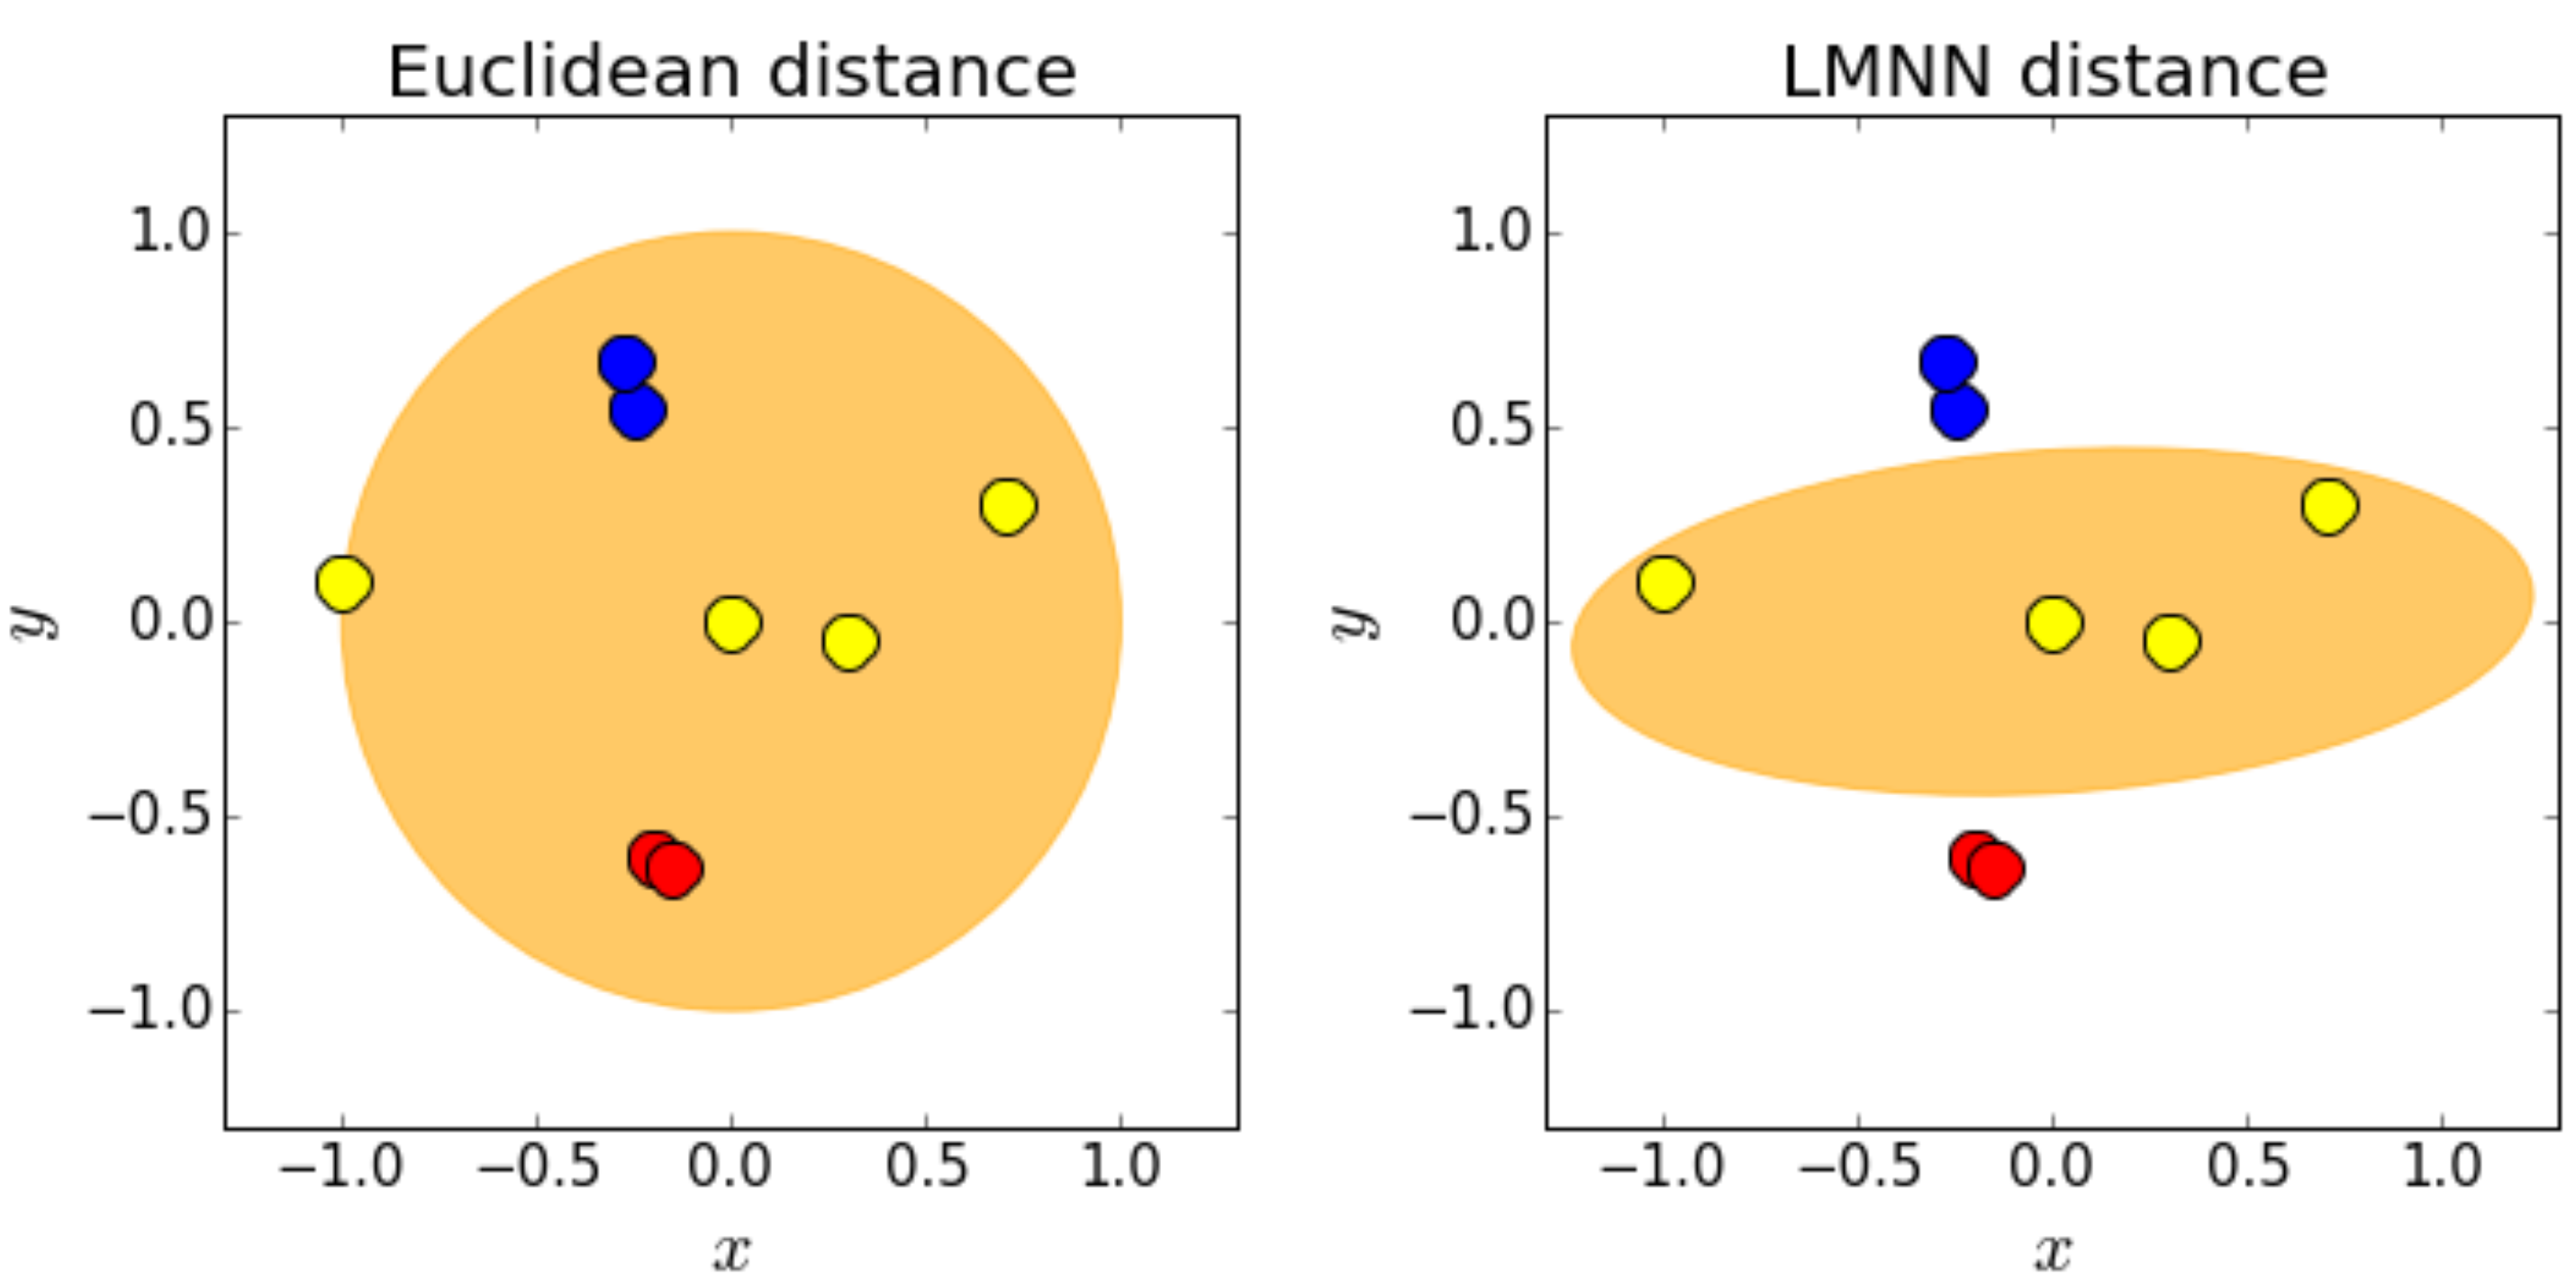
\includegraphics[width=0.9\linewidth]{figs/ch5/metric_learning_toy_example}
	\caption{Сравнение оптимальной метрики Махаланобиса алгоритма LMNN с евклидовой метрикой в двумерном случае}
	\label{ch5:fig:metric_learning_toy_example}
\end{figure}

\textbf{Классификация выравненных временных рядов в метрике Махаланобиса.}
Пусть $\mathbf{x} \in \mathbf{X}$~--- неразмеченный временной ряд. Выравниваем временной ряд $\mathbf{x}$ относительно всех центроидов классов
\[
	\mathbf{\hat{x}}_e = G(\mathbf{x}, \mathbf{c}_e), \quad \text{где} \quad e \in \{1, \dots, K\}.
\]
Отнесем временной ряд к классу, для которого минимально расстояние до соответствующего центроида. В качестве расстояния используем обученную метрику Махаланобиса с фиксированной матрицей $\mathbf{A}$
\[
	\hat{y} = \argmin_{e \in \bbY} d_\mathbf{A}(\mathbf{\hat{x}}_e, \mathbf{c}_e).
\]
После нахождения оптимальных центроидов классов и нахождения оптимальной матрицы трансформаций процедура классификации заключается в измерении расстояния между найденными центроидами и новыми неразмеченными объектами.

Для оценки качества работы алгоритма будем вычислять ошибку классификации как долю неправильно классифицированных объектов тестовой выборки~$\{ \bx_i, y_i \}_{i=1}^{\hat{m}}$:
\[
	\text{error} = \frac1{\hat{m}} \sum_{i = 1} ^ {\hat{m}} [a(\mathbf{x}_i) \ne y_i].
\]

%%%%%%%%%%%%%%%%%%%%%%%%%%%%%%%%%%%%%%%%%%%%%%%%
\textbf{Анализ метрического пространства для задачи кластеризации.}
\label{sec:ch5:exp_clustering}
%%%%%%%%%%%%%%%%%%%%%%%%%%%%%%%%%%%%%%%%%%%%%%%%

В целях проверки работоспособности предложенного подхода проведен вычислительный эксперимент на модельных данных. Сгенерирована выборка объектов, принадлежащих одному из двух классов, в двумерном пространстве.
Каждый объект принадлежит многомерному нормальному распределению.
На Рис.~\ref{ch5:fig:true_distr} показано истинное распределение объектов, черным цветом выделены истинные центры классов и линии уровня функции распределения.

Применим к данной выборке базовый алгоритм $k$-средних.
Результат кластеризации показан на Рис.~\ref{ch5:fig:kmeans_clustering}, где черным цветом выделены найденные центры классов и линии уровня функции распределения, построенной по выборочной матрице ковариаций.

Взяв за начальное приближение результаты работы алгоритма $k$-средних,
проведем клас\-те\-ри\-за\-цию с помощью алгоритма адаптивного метрического обучения.
Результаты работы алгоритма продемонстрированы на Рис.~\ref{ch5:fig:AML_clustering}.

На рисунках заметно улучшение результатов кластеризации.
Измеренная точность кластеризации алгоритма $k$-средних составила 0,76,
алгоритма адаптивного метрического обучения~--- 0,94, что говорит об эффективности данного подхода.

Таблица~\ref{ch5:tbl:clusteing_results} показывает результаты вычислительного эксперимента на реальных
данных.
Алгоритм был применен к $5$ выборкам, взятых из репозитория UCI~\cite{uci2017}.
Оценкой качества кластеризации служит число правильно кластеризованных объектов.
При кластеризации объектов на более чем два класса возникает проблема соотнесения истинных классов с полученными кластерами.
Данная проблема была формализована в виде задачи о назначениях и решена с помощью венгерского алгоритма. Вычислительный эксперимент на реальных данных показал увеличение точности кластеризации при использовании метрического обучения.

%%%%%%%%%%%%%%%%%%%%%%%%%%%%%%%%%%%%%%%%%%%%%%%%
\section{Анализ метрического пространства для задачи классификации временных рядов}
\label{sec:ch5:exp_classification}
%%%%%%%%%%%%%%%%%%%%%%%%%%%%%%%%%%%%%%%%%%%%%%%%
	Цель вычислительного эксперимента~--- проверить работоспособность предложенного подхода.
	Предполагается, что построенный алгоритм мультиклассовой классификации способен определить тип активности человека по форме сигнала акселерометра мобильного телефона.
	
	Для проведения базового вычислительного эксперимента были подготовлены синтетические временные ряды, принадлежащие двум классам.
	Первый класс~--- синусы вида $sin(x + b)$, где параметр $b$ определяет сдвиг каждого временного ряда.
	Второй класс~--- пилообразные функции с различными сдвигами по временной шкале.
	На каждый временной ряд был наложен нормальный шум.
	Число временных рядов каждого класса = 60.
	Длина каждого временного ряда $n = 50$.
	
	Построенные центроиды классов проиллюстрированы на Рис.~\ref{ch5:fig:centroids_synthetic}.
	Из рисунка видно, что процедура корректно определяет сдвиги временных рядов.
	
	Для того чтобы убедиться в целесообразности применения метрического обучения, данные
	временные ряды классифицировались в пространстве с евклидовой метрикой и в пространстве с метрикой Махаланобиса.
	Число ближайших соседей $k = 5$, размерность преобразованного пространства $p = 40$.
	Полученные ошибки классификации составили $27\%$ для евклидовой метрики и $6\%$ для метрики Махаланобиса.
	
	Реальные данные~\cite{wisdm} представляли собой временные ряды акселерометра мобильного телефона.
	Каждый из шести классов соответствовал определенной физической активности испытуемых.
	Для проведения вычислительного эксперимента было выбрано по $200$ объектов каждого класса.
	Длина каждого временного ряда равнялась $n = 128$ отсчетам времени.
	
	Построенные центроиды классов изображены на Рис.~\ref{ch5:fig:centroids_real}.
	Найденные центроиды обладают периодичностью, свойственной временным рядам показаний активности человека.
	На Рис.~\ref{ch5:fig:raw_ts} показаны примеры временных рядов каждого класса. Эти же временные ряды после процедуры выравнивания относительно построенных центроидов изображены на Рис.~\ref{ch5:fig:aligned_ts}.
	
	Ошибка классификации без использования метрического обучения составила~$37,5\%$.
	Алгоритм LMNN позволяет настроить параметры: число ближайших соседей~$k$,
	размерность преобразованного евклидова пространства~$p$.
	Для выбора оптимальных параметров воспользуемся процедурой кросс-валидации.
	На Рис.~\ref{ch5:fig:heat_map} цветом показана ошибка классификации алгоритма в зависимости от его параметров.
	На данной выборке алгоритм LMNN оказывается слабо чувствителен к числу ближайших соседей,
	и при уменьшении размерности пространства объектов ошибка классификации растет.
	
	Настроим алгоритм LMNN со следующими параметрами: число ближайших соседей $k = 30$, размерность
	выходного пространства $p = 128$.
	Ошибка классификации составила~$17,25\%$, что вдвое меньше ошибки классификации с использованием евклидовой метрики.
	
	В таблице~\ref{ch5:tbl:confussion_matrix} представлены матрицы несоответствий результатов классификации при использовании
	евклидовой метрики и метрики Махаланобиса.
	Столбцы соответствуют истинным меткам классов объектов, строки~--- предсказанным меткам.
	Диагональное преобладание матрицы несоответствий указывает на высокую предсказательную способность алгоритма.
	
	В таблице~\ref{ch5:tbl:improvement} продемонстрировано увеличение точности классификации при использовании в качестве меры расстояния метрики Махаланобиса.
	Пересечение $i$-го столбца и $j$-й строки отвечает изменению доли объектов класса $i$, отнесенных к классу $j$. Положительное суммарное значение диагональных элементов таблицы соответствует увеличению качества классификации. Значительное улучшение предсказания происходит при классификации первых трех классов.
	Данные классы соответствуют следующим видам физической активности: ходьба, ходьба вверх, ходьба вниз.
	
\textbf{Глава 6. Порождение признаков с помощью метамоделей}
\label{ch:metamodels}

Исходное пространство сигналов в задачах декодирования, а также в задачах анализа временных рядов является крайне избыточным и неинформативным.
Для извлечения информативных признаков в данной главе ставится задача порождения признакового пространства.

%%%%%%%%%%%%%%%%%%%%%%%%%%%%%%%%%%%%%%%%%%%%%%%%
\textbf{Постановка задачи порождения признакового пространства.}
\label{sec:ch6:feature_generation}
%%%%%%%%%%%%%%%%%%%%%%%%%%%%%%%%%%%%%%%%%%%%%%%%

Временные ряды акселерометра образуют множество~$\mathcal{S}$ сегментов~$\bs$ фиксированной длины~$T$:
\[
	\bs = [x_1, \dots, x_T]^{\T} \in \bbR^T.
\]
Необходимо построить модель классификации~$f: \bbR^T \rightarrow Y$, которая будет ставить в соответствие каждому сегменту из множества~$\mathcal{S}$ метку класса из конечного множества~$Y$.
Обозначим за
\begin{equation}
	\mathcal{D} = \{(\bs_i, y_i)\}_{i=1}^m
	\label{ch6:eq:sample}
\end{equation}
исходную выборку, где $\bs_i \in \mathcal{S}$ и $y_i = f(\bs_i)\in Y$.

Авторы предлагают построить модель~$f$ в в де суперпозиции $f=f(\mathbf{g})$.
Функция $\mathbf{g}: \bbR^T \rightarrow \bbR^n$ является отображением из пространства~$\bbR^{T} $ в признаковое пространство~$\mathbb{G} \subset \bbR^n$.
Имея функцию порождения признаков~$\mathbf{g}$, преобразуем исходную выборку~\eqref{ch6:eq:sample} в
\[
	\mathcal{D}_\mathbb{G} = \{(\mathbf{g}_i, y_i)\}_{i=1}^m,
\]
где $\mathbf{g}_i = \mathbf{g}(\bs_i) \in \mathbb{G}$. 

Модель классификации $f=f(\mathbf{g}, \btheta)$ является параметрической функцией с вектором параметров~$\btheta$. 
Оптимальные параметры~$\hat{\btheta}$ определяются оптимизацией функции ошибки классификации
\begin{equation}
	\hat{\btheta} = \argmin_{\btheta} L(\btheta, \mathcal{D}_\mathbb{G}, \bmu).
	\label{ch6:eq:optimal_classification_params}
\end{equation}
Вектор~$\bmu$ является внешним параметром для заданной модели классификации. 
Примеры таких параметров и функций ошибки для различных моделей классификации приведены ниже.

Чтобы сравнить качество классификации с прошлыми результатами~\cite{karasikov2016feature,ivkin2015ts}, в качестве метрики качества используется точность классификации:
\begin{equation}
	\mathrm{accuracy} = \frac{1}{m} \sum_{i=1}^{m} \left[f\left(\mathbf{g}(\bs_i), \hat{\btheta} \right)= y_i\right].
	\label{ch6:eq:accuracy}
\end{equation}

%%%%%%%%%%%%%%%%%%%%%%%%%%%%%%%%%%%%%%%%%%%%%%%%
\textbf{Модели порождения признакового пространства для временных рядов.}
\label{sec:ch6:feature_generation_models}
%%%%%%%%%%%%%%%%%%%%%%%%%%%%%%%%%%%%%%%%%%%%%%%%

Цель данной работы~--- провести сравнение различных подходов к генерации признаков.
В этом разделе проводится анализ рассматриваемых методов.

\textbf{Экспертные функции.}
В качестве базового подхода будем использовать экспертные функции как функции порождения признаков.
Экспертные функции~--- это некоторые статистики~$g_j$, где $g_j: \bbR^T \rightarrow \bbR$.
Признаковым описанием~$\mathbf{g}(\bs)$ объекта~$s$ являются значения заданных экспертных статистик для данного объекта
\[
	\mathbf{g}(\bs) = [g_1(\bs), \dots, g_n(\bs)]^{\T}.
\]

В работе~\cite{kwapisz2011activity} авторы предлагают использовать экспертные функции, приведенные в таблице~\ref{ch6:tbl:expert_functions}.
Такая процедура порождения признаков генерирует признаковое описание временного ряда~$\mathbf{g}(\bs) \in \bbR^{40}$.

\begin{table}[ht]
	\centering
	\caption{Примеры экспертных порождающих функций}
	\begin{tabular}{|l|c|}
		\hline
		\textbf{Function description}    & \textbf{Formula} \\ \hline
		Mean                    & $\bar{x} = \frac{1}{T} \sum_{t=1}^{T} x_t$    \\ \hline
		Standard deviation      & $\sqrt{\frac{1}{T} \sum_{t=1}^{T} (x_t - \bar{x})^2}$    \\ \hline
		Mean absolute deviation & $\frac{1}{T} \sum_{t=1}^{T} |x_t - \bar{x}|$    \\ \hline
		Distribution            &  Histogram values with 10 bins    \\ \hline
	\end{tabular}
	\label{ch6:tbl:expert_functions}
\end{table}

\textbf{Авторегрессионная модель.}
Авторегрессионная модель~\cite{lukashin2003adaptive} порядка~$n$
использует параметрическую модель для аппроксимации временного ряда~$\bs$. 
Каждое значение временного ряда приближается линейной комбинацией предыдущих $n-1$ значений
\begin{equation*}
	x_t = w_0 + \sum_{j=1}^{n-1} w_j x_{t-j} + \epsilon_t,
\end{equation*}
где $\epsilon_t$~--- регрессионные остатки.
Оптимальные параметры $\hat{\mathbf{w}}$ авторегрессионной модели используются как признаки $\mathbf{g}(\bs)$.
Данные параметры минимизируют квадратичную ошибку аппроксимации временного ряда и предсказания модели

\begin{equation}
	\mathbf{g}(\bs) = \hat{\mathbf{w}} = \argmin_{\mathbf{w} \in \bbR^{n}} \left( \sum_{t=n}^{T} \|x_t - \hat{x}_t\|^2\right).
	\label{ch6:eq:autoregressive_description}
\end{equation}
Задача~\eqref{ch6:eq:autoregressive_description} эквивалентна задаче линейной регрессии.
Поэтому для каждого временного ряда~$s$ необходимо решить задачу линейной регрессии размера $n$.
Пример аппроксимации временного ряда авторегрессионной моделью представлен на Рис.~\ref{ch6:fig:ar_example}.

\textbf{Анализ сингулярного спектра.}
Альтернативной гипотезой порождения признакового пространства для временного ряда является анализ сингулярного спектра (Singular Spectrum Analysis, SSA)~\cite{hassani2007singular}. 
Для каждого временного ряда~$\bs$ из исходной выборки~$\mathcal{D}$ строится траекторная матрица:
\[
	\mathbf{X} = 
	\begin{pmatrix}
		x_1 & x_2 & \dots & x_n \\
		x_2 & x_3 & \dots & x_{n+1} \\
		\dots & \dots & \dots & \dots \\
		x_{T-n+1} & x_{T-n+2} & \dots & x_T
	\end{pmatrix}.
\]
Здесь ширина окна $n$ является внешним структурным параметром.
Сингулярное разложение матрицы $\mathbf{X}^{\T} \mathbf{X}$:
\[
	\mathbf{X}^{\T} \mathbf{X} = \mathbf{U} \mathbf{\Lambda} \mathbf{U}^{\T},
\]
где $\mathbf{U}$~--- унитарная матрица и $\Lambda = \mathrm{diag}(\lambda_1, \dots, \lambda_n)$ причём $\lambda_i$ собственные значения $\mathbf{X}^{\T} \mathbf{X}$. 
Признаковое описание объекта $\bs$ задаётся спектром матрицы $\mathbf{X}^{\T} \mathbf{X}$:
\[
	\mathbf{g}(\bs) = \left[\lambda_1, \dots, \lambda_n\right]^{\T}.
\]
\textbf{Spline Approximation.}
Предлагаемый метод аппроксимирует временные ряды с помощью сплайнов~\cite{deboor1978splines}. Сплайн определяется его параметрами: узлами и коэффициентами.
Предполагается, что узлы сплайна $\{\xi_\ell\}_{\ell=0}^M$ равномерно распределены по временной оси.
Кусочные модели, построенные на отрезках $[\xi_{\ell-1}; \xi_{\ell}]$, заданы коэффициентами $\{\mathbf{w}_\ell\}_{\ell=1}^{M}$.
Оптимальные параметры сплайна являются решением системы с дополнительными условиями равенства производных до второго порядка включительно на концах отрезков.
Обозначим каждый отрезок-сегмент $p_i(t)$ $i = 1, \dots, M$ и весь сплайн $S(t)$. Тогда система уравнений принимает вид
\begin{align*}
	S(t) &= \begin{cases}
		p_1(t) = w_{10} +w_{11}t + w_{12}t^2 + w_{13}t^3, & t\in [\xi_0, \xi_1],\\
		p_2(t) = w_{20} +w_{21}t + w_{22}t^2 + w_{23}t^3, & t\in [\xi_1, \xi_2],\\
		\cdots&\cdots \\
		p_{M}(t) = w_{L0} +w_{M1}t + w_{M2}t^2 + w_{M3}t^3, & t\in [\xi_{M-1}, \xi_M],					
	\end{cases}
\end{align*}
\begin{align*}
	S(\xi_t) &= x_t, \quad t = 0, \dots, M,\\
	p_i'(\xi_i) &= p_{i+1}'(\xi_i),\: p_i''(\xi_i) = p_{i+1}''(\xi_i), \quad i = 1, \dots, M-1,\\
	p_i(\xi_{i-1}) &= x_{i-1},\: p_i(\xi_i) = x_i, \quad i = 1, \dots, M.
\end{align*}
Объединение всех параметров сплайна задаёт признаковое описание временного ряда:
\[
	\mathbf{g}(\bs) = \left[\mathbf{w}_1, \dots, \mathbf{w}_{M}\right]^{\T}.
\]

Рис.~\ref{ch6:fig:spline_example} показывает аппроксимацию временного ряда с использованием модели сплайнов.
По сравнению с авторегрессионной моделью сплайны строят более гладкую аппроксимацию, используя такое же количество параметров.

%%%%%%%%%%%%%%%%%%%%%%%%%%%%%%%%%%%%%%%%%%%%%%%%
\section{Классификация временных рядов в порожденном признаковом пространства}
\label{sec:ch6:feature_generation_classification}
%%%%%%%%%%%%%%%%%%%%%%%%%%%%%%%%%%%%%%%%%%%%%%%%

Для классификации временных рядов будем использовать подход один против всех. 
Для каждого класса обучается бинарный классификатор, и на стадии предсказания объект классифицируется согласно наиболее уверенному классификатору.
Использовались три модели классификации: логистическая регрессия, SVM и случайный лес.

\subsubsection{Логистическая регрессия.}
Оптимальные параметры модели $\hat{\mathbf{w}}, \hat{b}$  в случае логистической регрессии определяются минимизацией функции ошибки~\eqref{ch6:eq:optimal_classification_params}

\begin{equation*}
	L(\btheta, \mathcal{D}_\mathbb{G}, \mu) = \sum_{i=1}^{m} \log\bigl(1 + \exp(-y_i [\mathbf{w}^{\T} \mathbf{g}_i + b])\bigl) + \frac{\mu}{2} \|\mathbf{w}\|^2, \:\:\mbox{where}\:\: \btheta  = \begin{bmatrix}
	\mathbf{w} \\ b
	\end{bmatrix}.
\end{equation*}

Решающее правило $f(\mathbf{g}, \btheta)$~--- знак линейной комбинации описания объекта~$\mathbf{g}$ и параметров $\hat{\btheta}$
\begin{equation*}
	\hat{y} = f(\mathbf{g}, \hat{\btheta}) = \sgn(\mathbf{g}^{\T} \hat{\mathbf{w}} + \hat{b}).
\end{equation*}

\subsubsection{SVM.}
Оптимизационная задача метода SVM имеет вид
\begin{align*}
	\hat{\btheta}  = \begin{pmatrix}
	\hat{\mathbf{w}} \\ \hat{b} \\ \hat{\mathbf{\xi}}
	\end{pmatrix}= \argmin_{\mathbf{w}, b, \mathbf{\xi}}  \frac{1}{2} \|\mathbf{w}\|^2 + \mu \sum_{i=1}^{m} \xi_i,\:\:
	\mbox{s.t.} \:\: &y_i \left(\mathbf{w}^{\T} \mathbf{g}_i + b\right) \geq 1 - \xi_i,\\
	&\xi_i \geq 0, \quad 1 \leq i \leq m.
\end{align*}
Целевая функция соответствует функции ошибки классификации $L(\btheta, \mathcal{D}_\mathbb{G}, \mu)$.
Предсказание для нового объекта вычисляется аналогично $
\hat{y} = \sgn (\mathbf{g}^{\T} \hat{\mathbf{w}} + \hat{b})$.

\subsubsection{Случайный лес.}
Случайный лес использует идею бэггинга. 
Идея состоит в построении многих слабых, неустойчивых классификаторов на подвыборках с возвращениями и усреднения их предсказаний.
Метод предполагает использование в качестве базовых классификаторов моделей с низким смещением и высокой дисперсией. 
Усреднение позволяет уменьшить дисперсию.
В случае случайного леса базовой моделью выступают решающие деревья. Идея бэггинга используется не только для самих объектов, но и для множества признаков.
В данном случае предсказание для нового объекта получается усреднением всех предсказаний отдельных деревьев:

\begin{equation*}
	\hat{y} = \sgn \left(\frac{1}{B} \sum_{i=1}^{B} \text{pred}(\mathbf{g}_i) \right),
\end{equation*}
где $B$~--- количество деревьев в композиции.


%%%%%%%%%%%%%%%%%%%%%%%%%%%%%%%%%%%%%%%%%%%%%%%%
\textbf{Анализ порожденных признаковых пространств.}
\label{sec:ch6:exp_feature_generation}
%%%%%%%%%%%%%%%%%%%%%%%%%%%%%%%%%%%%%%%%%%%%%%%%

В данной работе эксперименты проводились на двух наборах данных временных рядов акселерометра мобильного телефона: WISDM~\cite{wisdm} и USC-HAD~\cite{usc}. 
Акселерометр мобильного телефона проводит измерение ускорения по трём осям с частотой 100 Hz.
Данные WISDM содержат 4321 временной ряд.
Каждый временной ряд принадлежит к одному из 6 классов. 
Данные USC-HAD содержат 13620 временных рядов, принадлежащих одному из 12 классов.  
В таблице~\ref{ch6:tbl:activities_distributions} представлено распределение временных рядов по классам для каждого датасета.
Длина временного ряда равна 200.
На Рис.~\ref{ch6:fig:ts_example} представлен пример одного из временных рядов.

\begin{figure}[!ht]
	\centering
	\subfloat{
		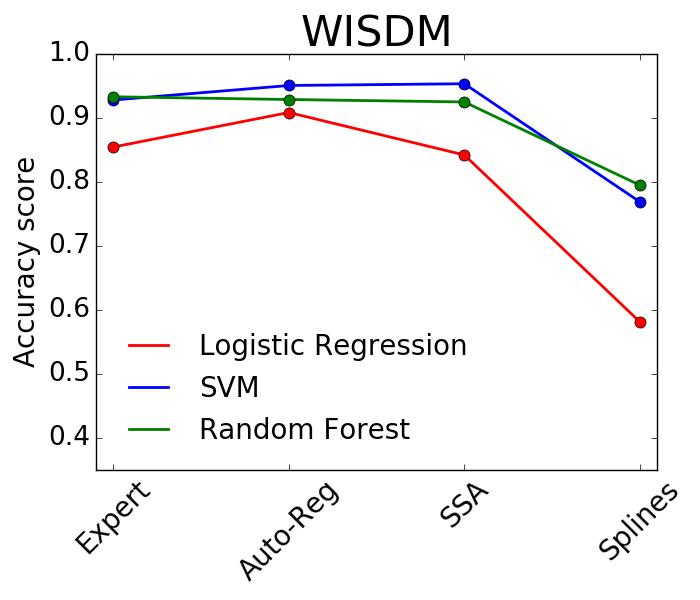
\includegraphics[width=0.49\linewidth]{figs/ch6/wisdm_methods.png}}
	\subfloat{
		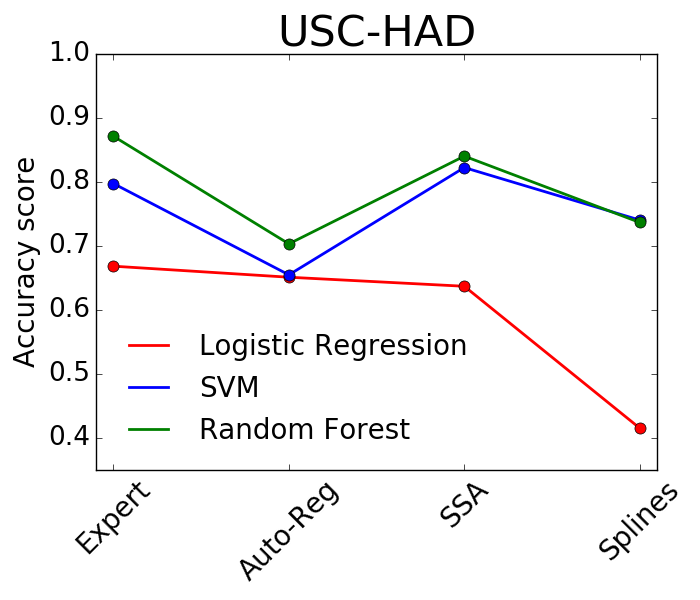
\includegraphics[width=0.49\linewidth]{figs/ch6/uschad_methods.png}}
	\caption{Мультиклассовая точность классификации для различных порожденных признаковых пространств}
	\label{ch6:fig:accuracy_results}
\end{figure}

В эксперименте для каждого набора данных были порождены признаки одним из методов: экспертные функции, авторегрессионная модель, SSA и сплайны.
Для каждой процедуры порождения признакового описания настраивались три модели классификации: логистическая регрессия, SVM и случайный лес.
Внешние структурные параметры (длина авторегрессионной модели $n$, ширина окна SSA $n$, число узлов сплайна $M$) настраивались процедурой кросс-валидации:
\begin{equation*}
	CV(K) = \frac{1}{K}\sum_{k=1}^{K} L(f_k, \mathcal{D}\setminus \mathcal{C}_k),
\end{equation*}
где $\mathcal{C}_k$~---$\frac{K-1}{K}$ доля от всей выборки, используемая для обучения модели $f_k$.
Гиперпараметры $\boldsymbol{\mu}$ моделей классификации были настроены той же процедурой кросс-валидации.

Первый подход к порождению признаков временных рядов~--- экспертные функции.
Основной недостаток такого подхода необходимость экспертного задания функций и возможности их вычисления для конкретного набора данных.

Авторегрессионная модель требует задания параметра длины модели $n$. 
Процедура кросс-валидации дала наибольшее качество при $n=20$ для обоих наборов данных.

Модель SSA была настроена аналогичной процедурой выбора оптимальных гиперпараметров. Конечная модель имела ширину окна $n=20$.

Для аппроксимации временных рядов кубическими сплайнами~\cite{deboor1978splines} использовалась библиотека $scipy$. 
Узлы сплайнов $\{\xi_{\ell}\}_{\ell = 1}^M$ были распределены равномерно по временной оси.
Значение параметра $M$ было подобрано на кросс-валидации.

Для обоих наборов данных процедуры порождения признаковых описаний дали следующие количества признаков: экспертные функции~--- 40; авторегрессионная модель~--- 60; анализ сингулярного спектра~--- 60; сплайны~--- 33.

\begin{table}[!ht]
	\centering
	\caption{Бинарная точность классификации для данных WISDM с использованием рассматриваемых алгоритмов: EX~--- Expert, AR~--- Auto-Reg, SSA and  SPL for Splines}
	\footnotesize
	\begin{tabular}{r|rrrr|rrrr|rrrr|}
		& \multicolumn{4}{c|}{\textbf{Logistic Regression}} & \multicolumn{4}{c|}{\textbf{Random Forest}} & \multicolumn{4}{c|}{\textbf{SVM}}          \\ \cline{2-13} 
		& EX   & AR   & SSA   & SPL  & EX  & AR & SSA & SPL & EX & AR & SSA & SPL \\ \hline
		All& 0.85 & 0.91 & 0.84 & 0.58 & 0.93 & 0.93 & 0.92 & 0.79 & 0.93 & 0.95 & 0.95 & 0.77 \\
		Standing& 0.99 & 0.98 & 1.00 & 0.95 & 1.00 & 0.99 & 1.00 & 0.99 & 0.99 & 0.98 & 1.00 & 0.96 \\
		Walking& 0.91 & 0.96 & 0.86 & 0.61 & 0.96 & 0.97 & 0.95 & 0.86 & 0.96 & 0.98 & 0.98 & 0.84 \\
		Upstairs& 0.91 & 0.95 & 0.91 & 0.89 & 0.96 & 0.96 & 0.96 & 0.90 & 0.96 & 0.98 & 0.97 & 0.89 \\
		Sitting& 0.99 & 0.98 & 1.00 & 0.99 & 1.00 & 0.99 & 1.00 & 1.00 & 0.99 & 0.98 & 1.00 & 1.00 \\
		Jogging& 0.98 & 0.99 & 0.99 & 0.80 & 0.99 & 0.99 & 0.99 & 0.92 & 0.99 & 0.99 & 0.99 & 0.93 \\
		Downstairs& 0.93 & 0.96 & 0.94 & 0.92 & 0.96 & 0.97 & 0.96 & 0.92 & 0.96 & 0.98 & 0.97 & 0.92 \\ \hline
	\end{tabular}
	\label{ch6:tbl:wisdm_methods_results}
\end{table}

\begin{table}[!ht]
	\centering
	\footnotesize
	\caption{Бинарная точность классификации для данных USC-HAD с использованием рассматриваемых алгоритмов: EX~--- Expert, AR~--- Auto-Reg, SSA and  SPL for Splines}
	\label{my-label}
	\begin{tabular}{r|rrrr|rrrr|rrrr|}
		& \multicolumn{4}{c|}{\textbf{Logistic Regression}} & \multicolumn{4}{c|}{\textbf{Random Forest}} & \multicolumn{4}{c|}{\textbf{SVM}}          \\ \cline{2-13} 
		& EX   & AR   & SSA   & SPL  & EX  & AR & SSA & SPL & EX & AR & SSA & SPL \\ \hline
		All& 0.67 & 0.65 & 0.64 & 0.41 & 0.87 & 0.70 & 0.84 & 0.74 & 0.80 & 0.65 & 0.82 & 0.74 \\
		Standing& 0.94 & 0.94 & 0.92 & 0.89 & 0.98 & 0.94 & 0.97 & 0.98 & 0.95 & 0.94 & 0.97 & 0.96 \\
		Elevator-up& 0.94 & 0.94 & 0.93 & 0.92 & 0.95 & 0.95 & 0.95 & 0.95 & 0.93 & 0.94 & 0.94 & 0.93 \\
		Walking-forward& 0.87 & 0.87 & 0.89 & 0.70 & 0.97 & 0.89 & 0.96 & 0.88 & 0.95 & 0.87 & 0.97 & 0.91 \\
		Sitting& 0.98 & 0.95 & 0.94 & 0.96 & 0.99 & 0.96 & 0.98 & 0.99 & 0.98 & 0.96 & 0.99 & 0.99 \\
		Walking-downstairs& 0.95 & 0.93 & 0.93 & 0.90 & 0.99 & 0.96 & 0.98 & 0.95 & 0.98 & 0.93 & 0.98 & 0.96 \\
		Sleeping& 1.00 & 0.98 & 0.99 & 1.00 & 1.00 & 0.98 & 1.00 & 1.00 & 1.00 & 0.98 & 1.00 & 1.00 \\
		Elevator-down& 0.94 & 0.94 & 0.94 & 0.91 & 0.95 & 0.95 & 0.95 & 0.95 & 0.93 & 0.94 & 0.94 & 0.93 \\
		Walking-upstairs& 0.94 & 0.95 & 0.93 & 0.92 & 0.98 & 0.95 & 0.98 & 0.96 & 0.98 & 0.95 & 0.98 & 0.96 \\
		Jumping& 0.99 & 0.99 & 1.00 & 0.97 & 1.00 & 0.99 & 1.00 & 0.99 & 1.00 & 0.99 & 0.97 & 0.99 \\
		Walking-right& 0.91 & 0.90 & 0.91 & 0.86 & 0.97 & 0.92 & 0.96 & 0.92 & 0.96 & 0.90 & 0.97 & 0.93 \\
		Walking-left& 0.89 & 0.91 & 0.90 & 0.88 & 0.97 & 0.93 & 0.97 & 0.93 & 0.95 & 0.91 & 0.97 & 0.93 \\
		Running& 0.99 & 0.99 & 0.99 & 0.92 & 1.00 & 0.99 & 1.00 & 0.97 & 1.00 & 1.00 & 0.95 & 0.98\\ \hline
	\end{tabular}
	\label{ch6:tbl:uschad_methods_results}
\end{table}

На Рис.~\ref{ch6:fig:accuracy_results} показано качество классификации~\eqref{ch6:eq:accuracy} для двух наборов данных.
Для данных WISDM сплайны дали самое слабое качество классификации.
Результаты для экспертных функций, авторегрессионной модели и SSA схожи.
Для данных USC-HAD результат более восприимчив к выбору модели классификации. 
Для обоих наборов данных логистическая регрессия продемонстрировала наименьшее качество, SVM и случайный лес показали почти одинаковое качество.
Для набора данных USC-HAD модель с использованием аппроксимации сплайнами
показала сравнимое с другими методами качество. 

В таблицах~\ref{ch6:tbl:wisdm_methods_results} и~\ref{ch6:tbl:uschad_methods_results} представлены результаты классификации~\eqref{ch6:eq:accuracy} для каждого класса в отдельности.
Первая строка в обеих таблицах демонстрирует точность по всем классам для каждой модели и процедуры генерации признаков.
Следующие строки соответствуют бинарным точностям по каждому из классов.
Для данных WISDM лучшее качество имеют наименее активные классы, такие как Standing и Sitting. 
Для USC-HAD заметного выделения качества для определенных классов не наблюдается.

Также был проведён эксперимент с использованием объединённого множества всех 193 сгенерированных признаков.
Результаты представлены на Рис.~\ref{ch6:fig:feature_union_results}. Соответствие между номера классов и видами активности приведено в таблице~\ref{ch6:tbl:activities_distributions}. 
Объединение признаков для обучения одной модели позволило увеличить качество. 
Для данных WISDM все точности классификации по классам больше $97 \%$, а для USC-HAD выше $93 \%$.

\textcolor{red}{ПРО ЗАКЛЮЧЕНИЕ}

\subsection*{Публикации соискателя по теме диссертации}
Публикации в журналах из списка ВАК.
\vspace{0.3cm}
\begin{enumerate}
	\item Исаченко Р. В., Стрижов В. В. Метрическое обучение в задачах мультиклассовой классификации временных рядов // Информатика и её применения, 2016. Т. 10. № 2. С. 48--57.
	\item Isachenko R. et al. Feature Generation for Physical Activity Classification // Artificial Intelligence and Decision Making, 2018. № 3. С. 20--27.
	\item Isachenko R. V., Strijov V. V. Quadratic programming optimization with feature selection for nonlinear models // Lobachevskii Journal of Mathematics, 2018. Т. 39. № 9. С. 1179--1187.
	\item Isachenko R. V., Vladimirova M. R., Strijov V. V. Dimensionality Reduction for Time Series Decoding and Forecasting Problems //DEStech Transactions on Computer Science and Engineering, 2018. №. optim.
	\item Исаченко Р.В., Яушев Ф.Ю., Стрижов В.В. Модели согласования скрытого пространства в задаче прогнозирования // Системы и средства информатики, 2021. Т. 31. № 1.
\end{enumerate}

\vspace{0.4cm}
{Прочие публикации.}
\vspace{0.2cm}
\begin{enumerate}
\setcounter{enumi}{5}
	\item Исаченко Р. В., Катруца А. М. Метрическое обучение и снижение размерности пространства в задачах кластеризации // Машинное обучение и анализ данных, 2016. T. 2. № 1. С. 17--25.
\end{enumerate}

\end{document}